\documentclass[withoutpreface,bwprint]{cumcmthesis} %去掉封面与编号页,电子版提交的时候使用。
\usepackage{bm}
\usepackage{appendix}
\usepackage[framemethod=TikZ]{mdframed}
\usepackage{url}   % 网页链接
\usepackage{subcaption} % 子标题
\usepackage{array}
\usepackage{graphicx}
\usepackage{caption}
\usepackage{float}
\usepackage{natbib}
\usepackage{enumitem}
\usepackage{booktabs}
\usepackage{pdfpages}
\usepackage{graphicx}

\usetikzlibrary{decorations.pathreplacing} % 用于添加大括号的库

\begin{document}
\title{编者注}

\maketitle
首先恭喜大家通过了前面的考核,选择了加入视觉/算法组。   

机器视觉是当前计算机发展的一个重要的研究方向,它旨在实现机器人对环境进行更加详细地感知。
由于可见光在成像方面清晰度、成像速度方面等具有很好的优势,因此机器视觉的研究也逐渐成为计算机视觉领域的研究热点。
在技术发展过程中,计算机视觉的技术可以大体分为两个技术方向,即图像处理与机器学习。

\textbf{图像处理}是指通过计算机对图像进行分析、处理、识别、理解等,从而实现对图像的高效、准确的描述、分析和理解。
主要的方法是通过计算机算法对图像进行处理,如图像增强、图像分割、图像检索、图像配准、图像修复、图像检索、图像分类、图像检索、图像压缩等。
在实际的应用场景中具有性能开销小,运算速度快,开发成本低等优点。

\textbf{机器学习}是指通过神经网络对图像进行分析。今年来随着深度学习和卷积神经网络的发展,机器学习技术也越来越多的应用于计算机视觉中。
机器学习的主要方法是通过训练数据对计算机模型进行训练,使计算机能够对未知数据进行预测、分类、聚类、回归等。
在图像处理中,机器学习可以应用于图像分类、目标检测、图像分割、图像检索、图像配准、图像修复等。
也涌现出了一大批优秀的物体识别算法,如YOLO等。

在实际的应用场景中,两种方法不是互相孤立的,而是需要我们相互结合,取长补短,才能达到更好的效果。除此之外,
光有计算机视觉也是远远不够的,
在现实的生产生活中,制造机器人主要的目的是为了达到自动化,面对真正的项目,
一般都是在一个miniPC中实现控制理论和多个数据融合处理,之后配合若干下位机进行自动化地完成任务。
所以代码、算法以及一些控制理论只是我们的工具,真正的目标是多感官的融合和自动化的控制。

俗话说“工欲善其事,必先利其器”,只有我们对基本的编程语言,对计算机的行为逻辑,对硬件作用与联系有着深刻的理解,
才能更好地理解每一种算法的特点,更好地洞悉每种操作背后的原理。从而应用到实际,切实地提高我们的创新能力和解决问题的能力。

在我们的培训中,我们将由浅入深,细致地为大家讲解机器视觉的知识,让大家能够更加深入地理解图像处理与机器学习的原理,
并运用到实际的项目中,提升自己的能力。在接下来的学习中,我们将更加注重理论知识的学习,重点讲解机器视觉的理论基础,
以及如何运用到实际的项目中。

送同学们一首我非常喜欢的诗:

\textbf{天高云淡, 望断南飞雁。 不到长城非好汉, 屈指行程二万。} 

\textbf{六盘山上高峰, 红旗漫卷西风。 今日长缨在手, 何时缚住苍龙?}

最后,祝大家学习愉快,工作顺利!

\newpage

\tableofcontents
\footnote{表星号的内容属于选修内容}
\newpage

\section{走进Linux系统}

linux操作系统是视觉后续工作的重要载体,因此熟悉linux系统的相关操作显得尤为重要。本节中将从安装双系统入手带大家逐步熟悉linux系统的基本操作。

\subsection{安装ubuntu22.04双系统}

本部分以windows11系统为例进行安装说明,如有使用特殊体质mac系统还请寻找其他方法(也许后续会补充进来)。
安装双系统主要分为以下四个流程:windows系统分区,制作启动盘,从U盘进行安装,系统设置相关。下面将进行一一说明。
\subsubsection{windows系统分区}
右键桌面上的“此电脑”图标,点击“管理”选项,进入“磁盘管理”界面,在这里你会看到电脑上存在若干个磁盘分区如下图所示。

\begin{figure}[H]
    \centering
    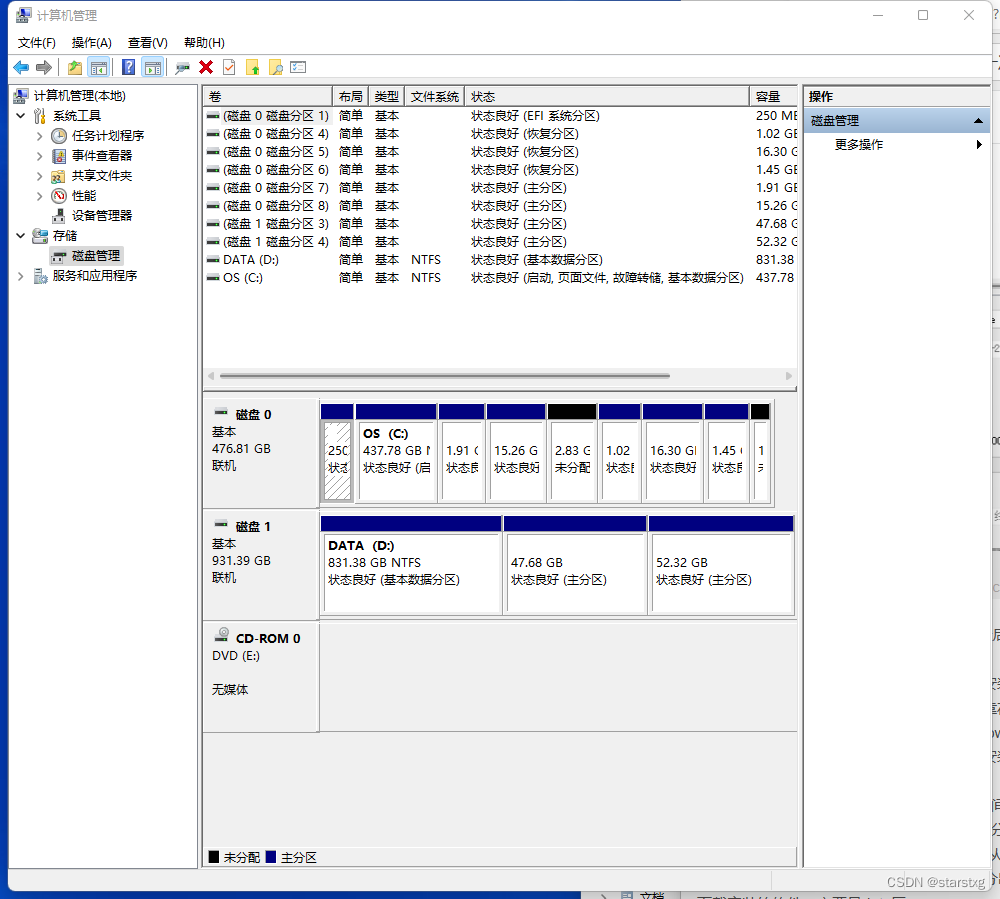
\includegraphics[width=0.7\textwidth]{linux1.png}
    \caption{磁盘分区} % 图片标题
    \label{fig:linux1} % 图片标签,用于引用
\end{figure}

选择一个剩余空间较大的磁盘,右击,点击“压缩卷”,等待计算完成后会显示当前磁盘中可用的压缩空间大小。输入你要留给ubuntu系统的空间量(注意是以MB为单位的),推荐是预留200G,后续内存不够虽然可以扩容但操作起来有点麻烦。

\begin{figure}[H]
    \centering
    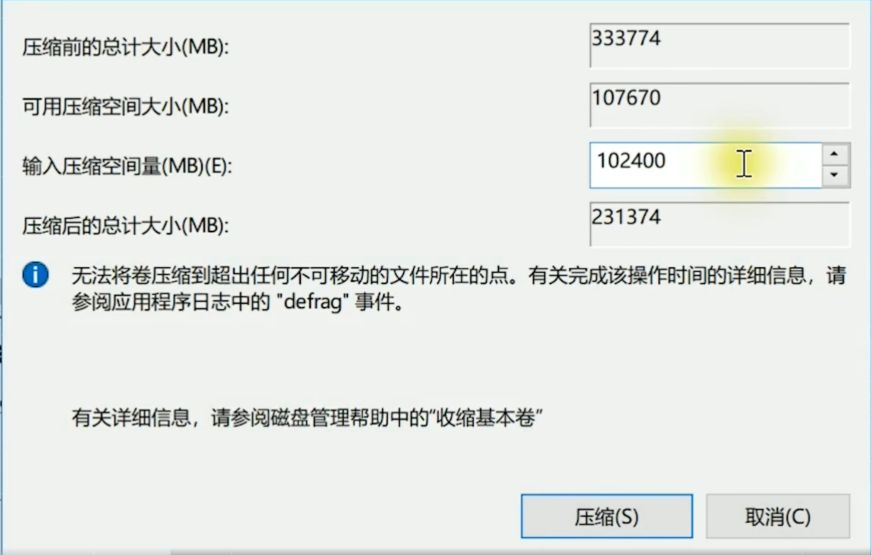
\includegraphics[width=0.7\textwidth]{linux2.jpg}
    \caption{分配linux空间} % 图片标题
    \label{fig:linux2} % 图片标签,用于引用
\end{figure}

输入好后点击“压缩”,压缩完成后出现一个“未分配”的区域则说明分区完成。

\subsubsection{制作启动盘}
首先需要一个内存大于16GB的U盘,请先对其中的文件进行备份,后续操作需要格式化这个U盘。

然后进入ubuntu官网下载ubuntu22.04版本的镜像,下载链接为

\url{https://ubuntu.com/download/alternative-downloads}

注意是下载22.04.5 Desktop!

下载好后还需要下载一个软碟通来将刚刚的ISO写入U盘中,下载链接

\url{https://www.ultraiso.net/xiazai.html} 

打开软碟通点击“继续试用”即可,不需要订购。进入软碟通界面,点击左上角的“文件”-\textgreater“打开”,选择刚刚下载的ISO镜像。点击“启动”-\textgreater“写入硬盘映像”,在弹出窗口的“硬盘驱动器”选项栏中确定是自己现在插上的U盘,写入方式选择USB-HDD+。

\begin{figure}[H]
    \centering
    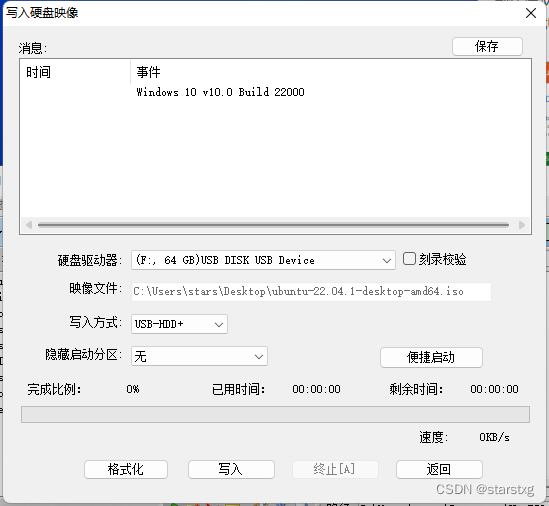
\includegraphics[width=0.7\textwidth]{linux3.png}
    \caption{制作启动盘} % 图片标题
    \label{fig:linux3} % 图片标签,用于引用
\end{figure}

然后对硬盘进行格式化,文件系统选择FAT32(默认),格式化完成后点击“写入”,等待写入完成。

\begin{figure}[H]
    \centering
    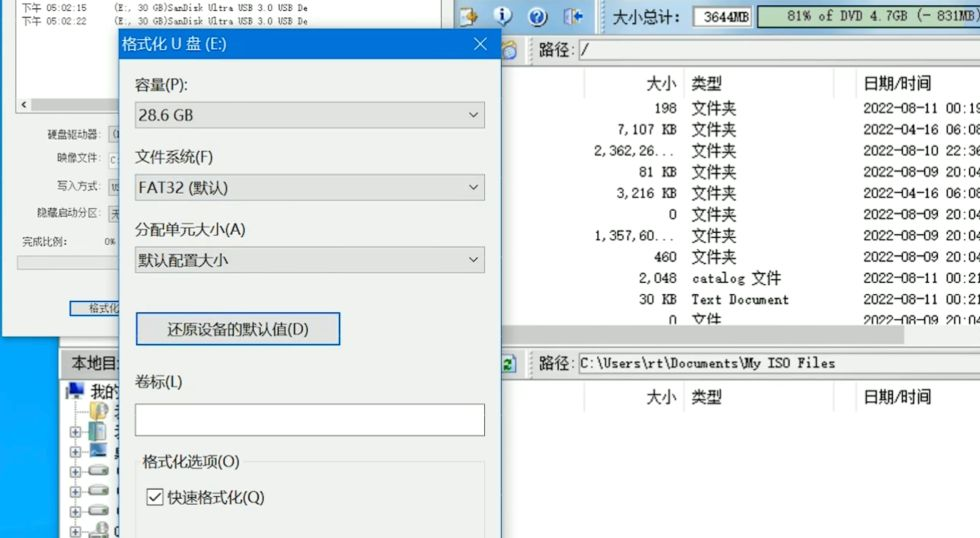
\includegraphics[width=0.7\textwidth]{linux4.jpg}
    \caption{U盘格式化} % 图片标题
    \label{fig:linux4} % 图片标签,用于引用
\end{figure}

U盘被制作成启动盘后仍可以存放其它的文件,插到windows中会提示该U盘有问题建议修复之类的,U盘没坏的话这时候不用管它就好。启动盘被称为“数字生命”,所以请好好保存。
\subsubsection{从U盘进行安装}
插入之前做好的启动盘,重启电脑,重启时快速重复按下启动选项快捷键,各个主板的启动选项快捷键有所不同,可以参考下表进行操作。

\begin{figure}[H]
    \centering
    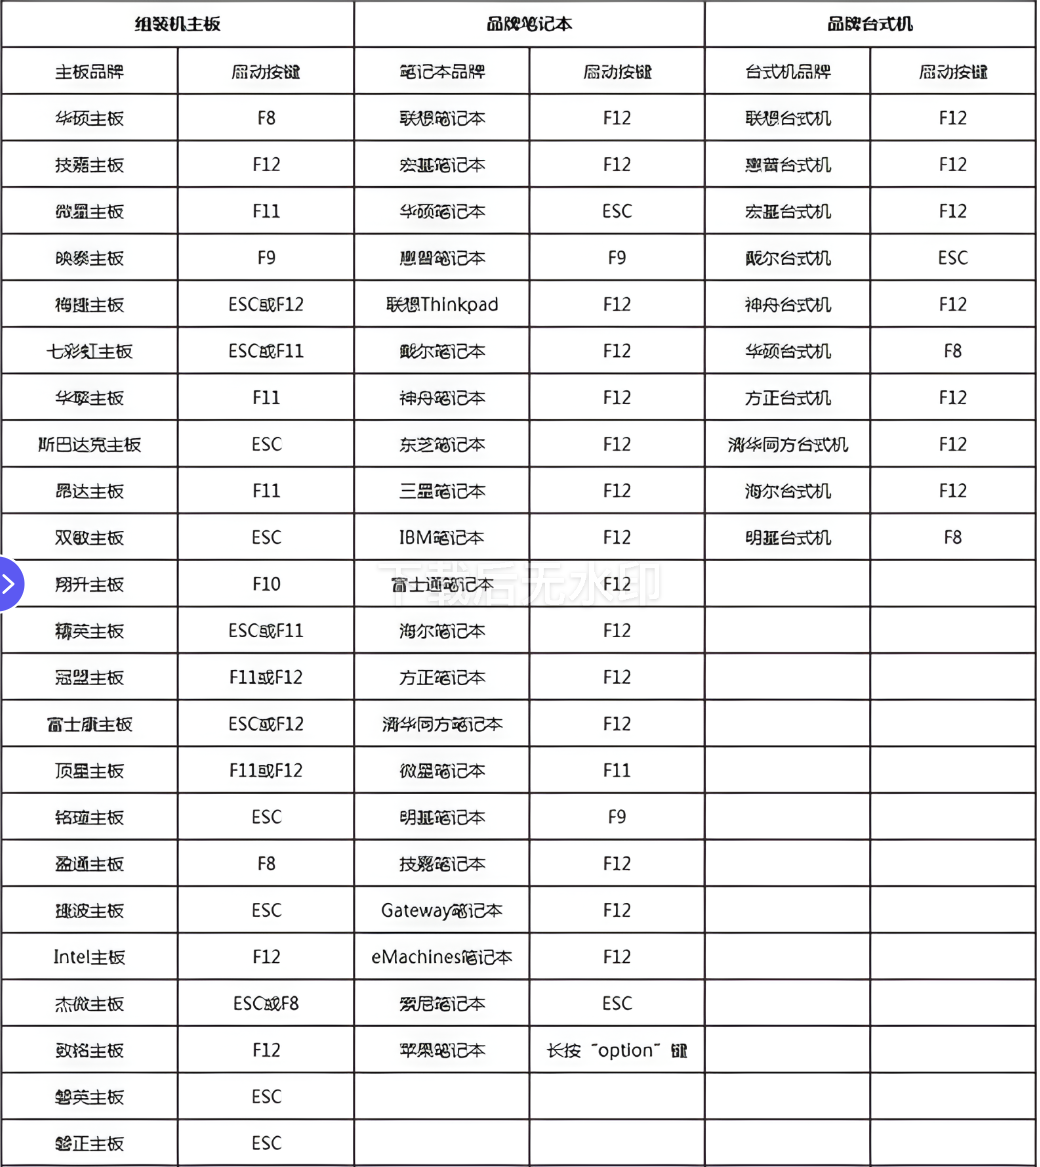
\includegraphics[width=0.7\textwidth]{install1.png}
    \caption{启动选项快捷键一览} % 图片标题
    \label{fig:install1} % 图片标签,用于引用
\end{figure}

进入启动选项界面后通过上下键选择Linpus lite选项,回车,进入系统安装程序,选择Try or Install Ubuntu,再回车,现在你离成功安装ubuntu双系统只有一步之遥啦。

\begin{figure}[H]
    \centering
    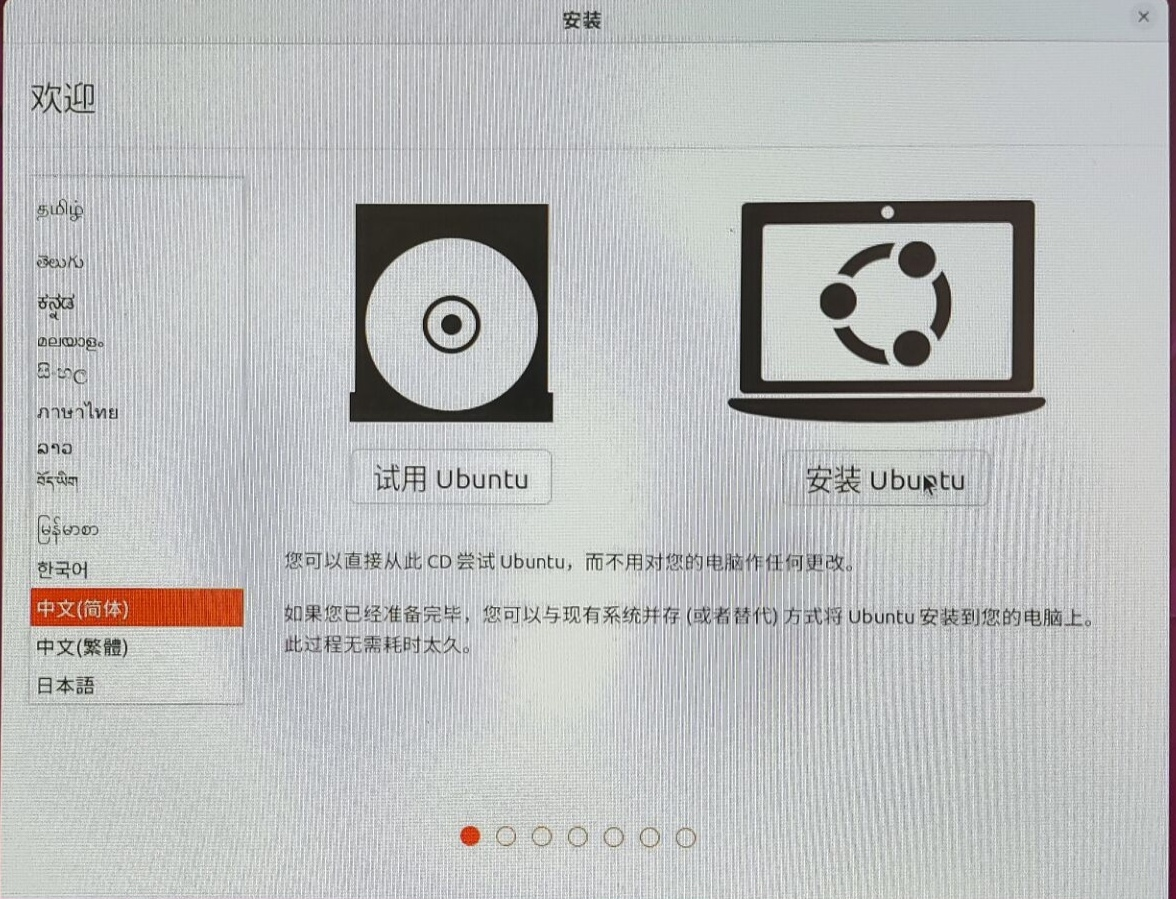
\includegraphics[width=0.7\textwidth]{install2.jpg}
    \caption{开始安装ubuntu} % 图片标题
    \label{fig:install2} % 图片标签,用于引用
\end{figure}

进入安装环节,首先选择语言为简体中文,点击“安装Ubuntu”,“键盘布局”确认是中文就好,下一步无线连接现在不用连。“更新和其他软件”界面选择“正常安装”,勾选“为图形或无线硬件,以及其它媒体格式安装第三方软件”并设置自己用户的密码,注意这个密码后面会经常用到,所以不建议设的过长。

\begin{figure}[H]
    \centering
    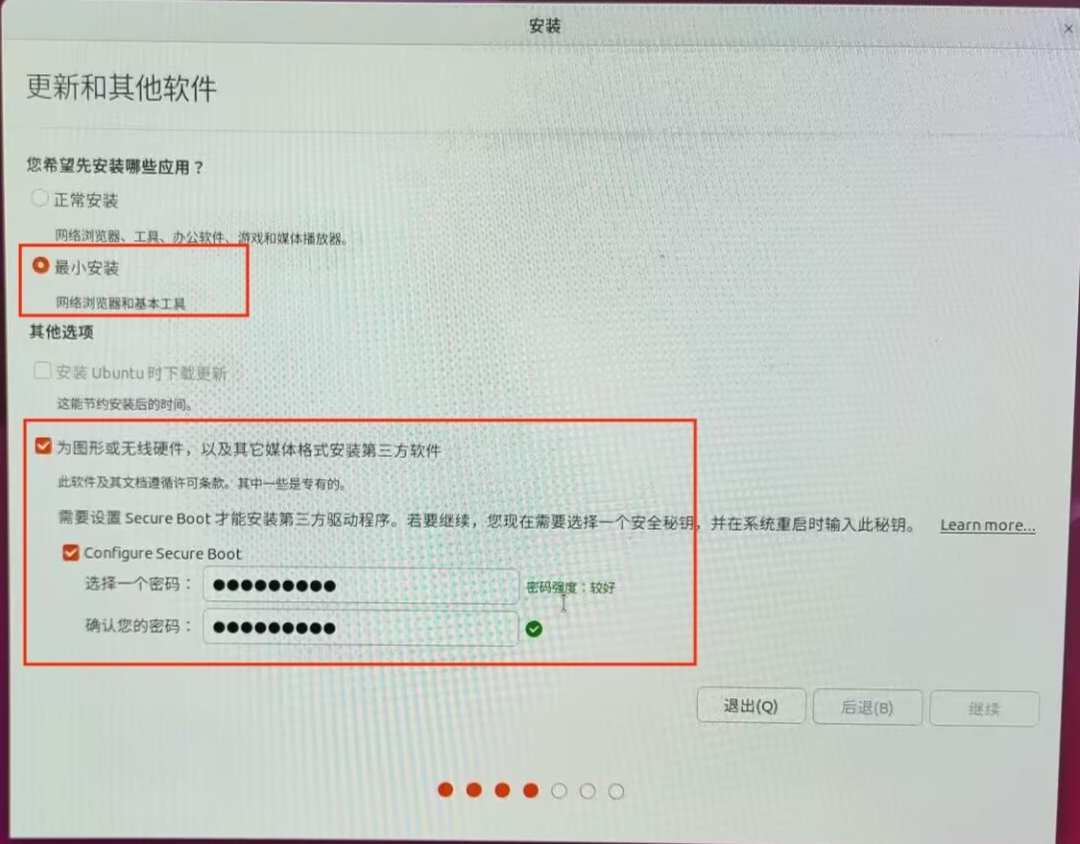
\includegraphics[width=0.7\textwidth]{install3.jpg}
    \caption{设置密码} % 图片标题
    \label{fig:install3} % 图片标签,用于引用
\end{figure}

在下一步“安装类型”中一定一定要选择“其它选项”!!!

然后来到“安装类型”,在这里我们需要创建ubuntu的分区(注意内存大小依然是以MB为单位)并挂载到相应的挂载点上。这里有两种方法:
\begin{enumerate}
	\item \textbf{全部挂载到根目录下}

找到之前压缩出来的空闲区域,双击选项,在弹出窗口的挂载点一栏输入/即可。这种方式最直接、最无脑,适合啥也不明白的新手操作,但是不利于多个分区的内存分配,在备份系统镜像的时候也无法按照不同分区分开备份,因此建议还是按照第二种方法进行分区。
	\item \textbf{挂载到不同目录下}

先分逻辑分区,再分主分区。
	\begin{enumerate}
		\item /boot启动分区:逻辑分区,一般选择200M-2G,放置Ubuntu的启动引导文件。
		\item /swap交换分区(虚拟内存):逻辑分区,一般分16GB就够了。
		\item / 根分区(root分区):逻辑分区,80GB左右差不多。
		\item /home分区:主分区,剩下的内存一起分给/home就好,平时文件也都放这边,要的内存最大。
	\end{enumerate}

点击压缩的空闲区域,点击左下角的加号

\begin{figure}[H]
    \centering
    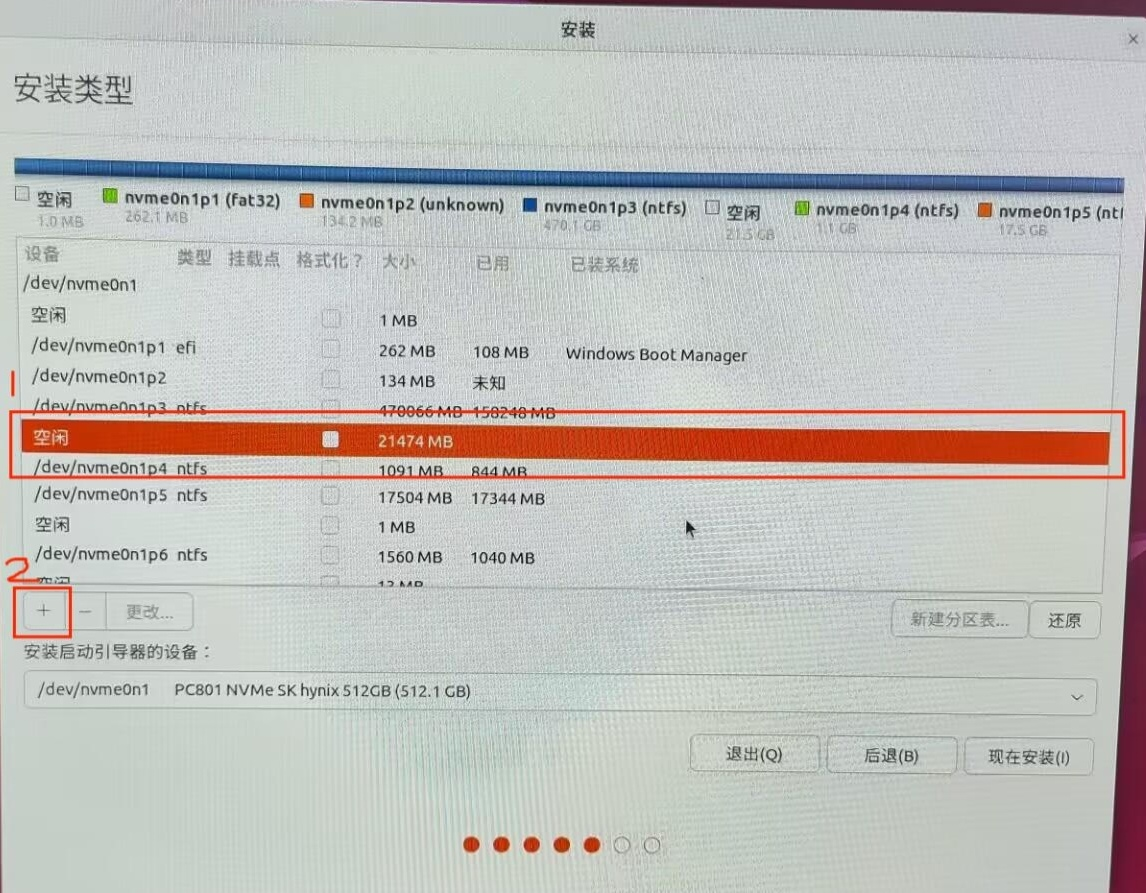
\includegraphics[width=0.7\textwidth]{install4.jpg}
    \caption{选择分区} % 图片标题
    \label{fig:install4} % 图片标签,用于引用
\end{figure}

在弹出的窗口选择大小,新分区类型,新分区位置,文件系统类型,挂载点,依次对/boot,/swap,/,/home进行分区

\begin{figure}[H]
    \centering
    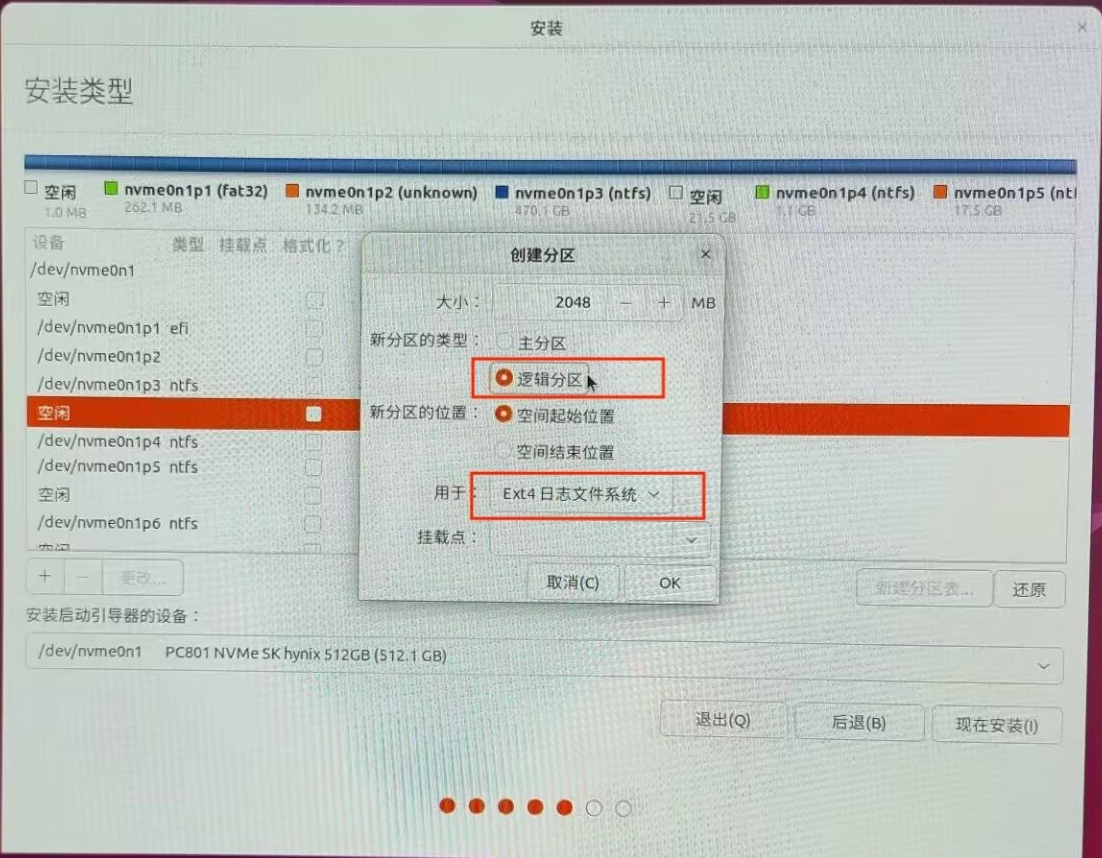
\includegraphics[width=0.7\textwidth]{install5.jpg}
    \caption{分区} % 图片标题
    \label{fig:install5} % 图片标签,用于引用
\end{figure}

再次确定安装启动引导盘的设备选择/boot分区那个路径

\begin{figure}[H]
    \centering
    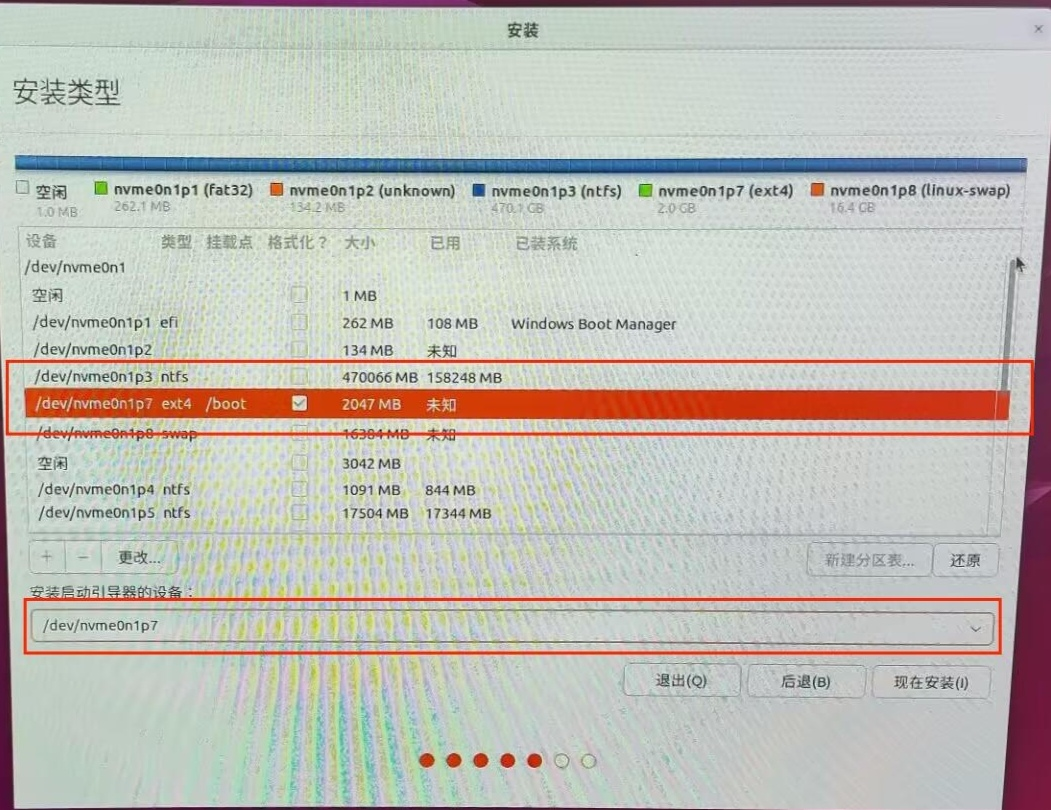
\includegraphics[width=0.7\textwidth]{install6.jpg}
    \caption{安装启动引导盘设备路径} % 图片标题
    \label{fig:install6} % 图片标签,用于引用
\end{figure}

\end{enumerate}
分区完成后点击“现在安装”,选择时区上海就行了。然后填写用户名和计算机密码,如果在上一步中填过了就不需要再填了。

点击“继续”,系统就会对ubuntu系统开始安装了,出现安装完成的提示后点击“现在重启”,等待一会,出现提示“Please remove the installation medium,then press ENTER”后拔掉启动盘并按下ENTER键,进入ubuntu系统的启动引导。在启动页面选择Ubuntu,电脑正常启动后就会进入Ubuntu系统,至此安装就全部完成啦。

ubuntu系统初始是一个什么都没有的状态,但是大家配好了也是可以和windows一样的,接下来各位就按照自己的习惯和喜好进行配置吧。

\subsubsection{系统设置相关}
ubuntu系统安装完成后你的默认启动系统会变成ubuntu,而有的电脑无法通过ubuntu的启动引导进入windows系统,这时候我们要怎样切换回windows系统呢?

首先重启电脑,重启时快速重复按下启动选项快捷键,进入启动引导,在这里选择windows系统即可启动windows。如果常用的系统还是windows,想优先启动windows系统,可以进入BOIS修改启动顺序。进入BIOS依然需要重启电脑,重启时快速重复按下进入BIOS的快捷键,各个主板的快捷键有所不同,可以参考下表进行操作。

\begin{figure}[H]
    \centering
    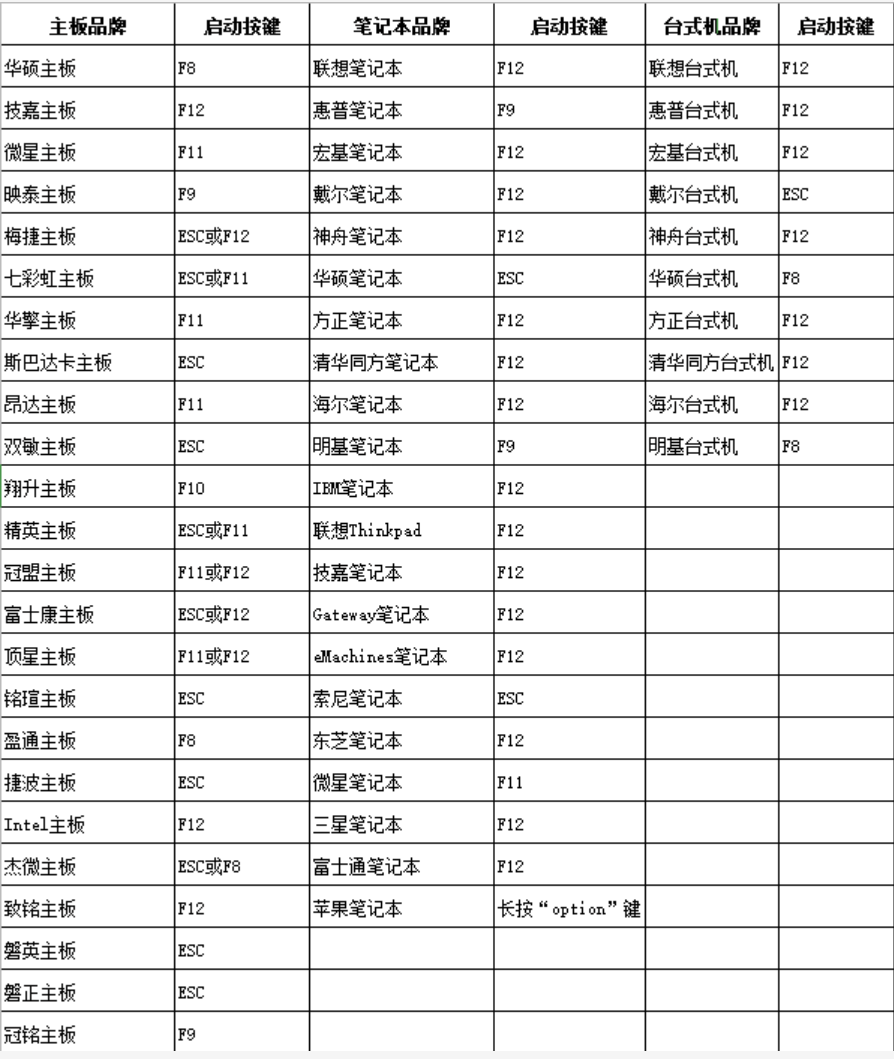
\includegraphics[width=0.7\textwidth]{install7.png}
    \caption{BIOS快捷键一览} % 图片标题
    \label{fig:install7} % 图片标签,用于引用
\end{figure}

进入BIOS后找到Boot相关设置,根据电脑提示将Windows Boot Manager移到ubuntu的启动引导上方,保存退出即可。

既然已经进入了BIOS,还有一点需要注意。如果你的电脑中安装了显卡,那在使用ubuntu之前请在BIOS中将显卡选择为“混合模式”而非“独立显卡”,否则可能出现启动ubuntu后黑屏加载不出来画面的情况。

\subsubsection{系统拓容}

如果系统中的文件已经多到内存爆炸了,那么此时我们就需要给ubuntu系统进行扩容。

扩容使用ubuntu自带的gparted分区管理工具,打开终端,输入

\begin{tcode}
	sudo apt-get install gparted
\end{tcode}

安装完成后输入

\begin{tcode}
	sudo gparted
\end{tcode}

进入gparted图形化界面,可以看到这里显示了电脑中的ubuntu和windows的所有分区,选中你要扩容的ubuntu分区,可以看到上方有一个箭头形状的图标亮起

\begin{figure}[H]
    \centering
    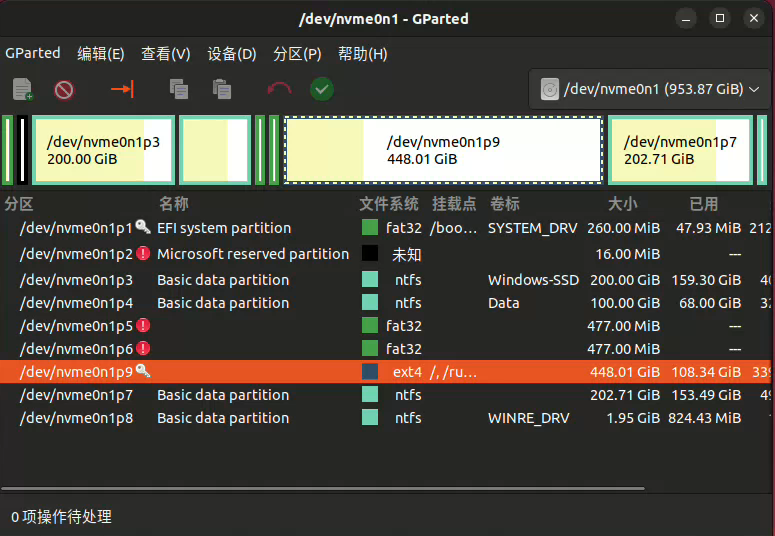
\includegraphics[width=0.7\textwidth]{linux10.png}
    \caption{gparted图形化界面} % 图片标题
    \label{fig:linux10} % 图片标签,用于引用
\end{figure}

点击箭头图标却发现以下报错:

\begin{figure}[H]
    \centering
    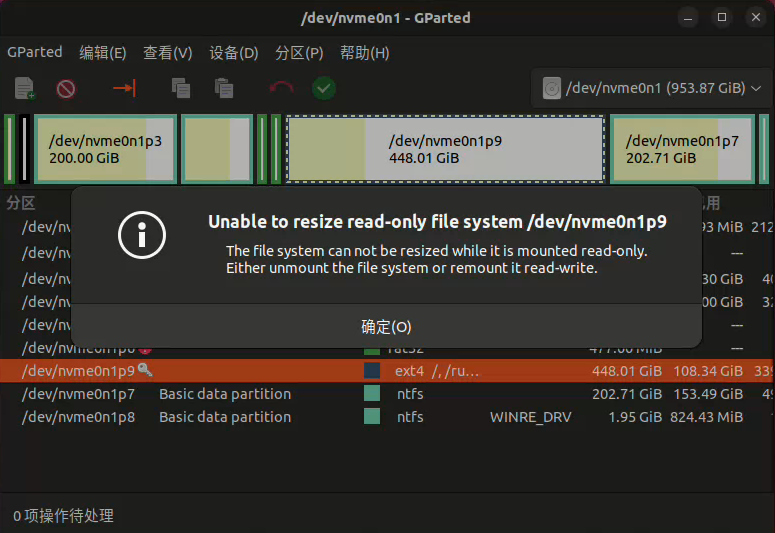
\includegraphics[width=0.7\textwidth]{linux9.png}
    \caption{gparted扩容失败} % 图片标题
    \label{fig:linux9} % 图片标签,用于引用
\end{figure}

这是因为当你处于ubuntu系统时,ubuntu相关的分区是被上锁的,此时你无法对分区进行修改。不过既然在ubuntu系统中不能修改ubuntu的分区,那么切换到别的系统时就可以修改ubuntu的分区。因此我们采取的方法是切换到试用的ubuntu系统再对自己的ubuntu分区进行修改。

在切换之前还有一件事要做:删除linux-swap和extend分区(如果存在的话),这是因为使用gparted扩容时只能对相邻的分区进行操作,如果swap和extend分区挡在ubuntu分区和windows分区之间,那么就不能从这个windows分区中分出内存给ubuntu分区了,因此要先删除这两个分区。

删除之后插上安装ubuntu系统时制作的启动盘,重启电脑,重启时快速重复按下启动选项快捷键。进入启动选项界面后通过上下键选择Linpus lite选项,回车,进入系统安装程序,选择Try or Install Ubuntu,再回车,这些步骤和安装ubuntu时是一样的,只是进入安装页面后,这次我们要选择试用Ubuntu

\begin{figure}[H]
    \centering
    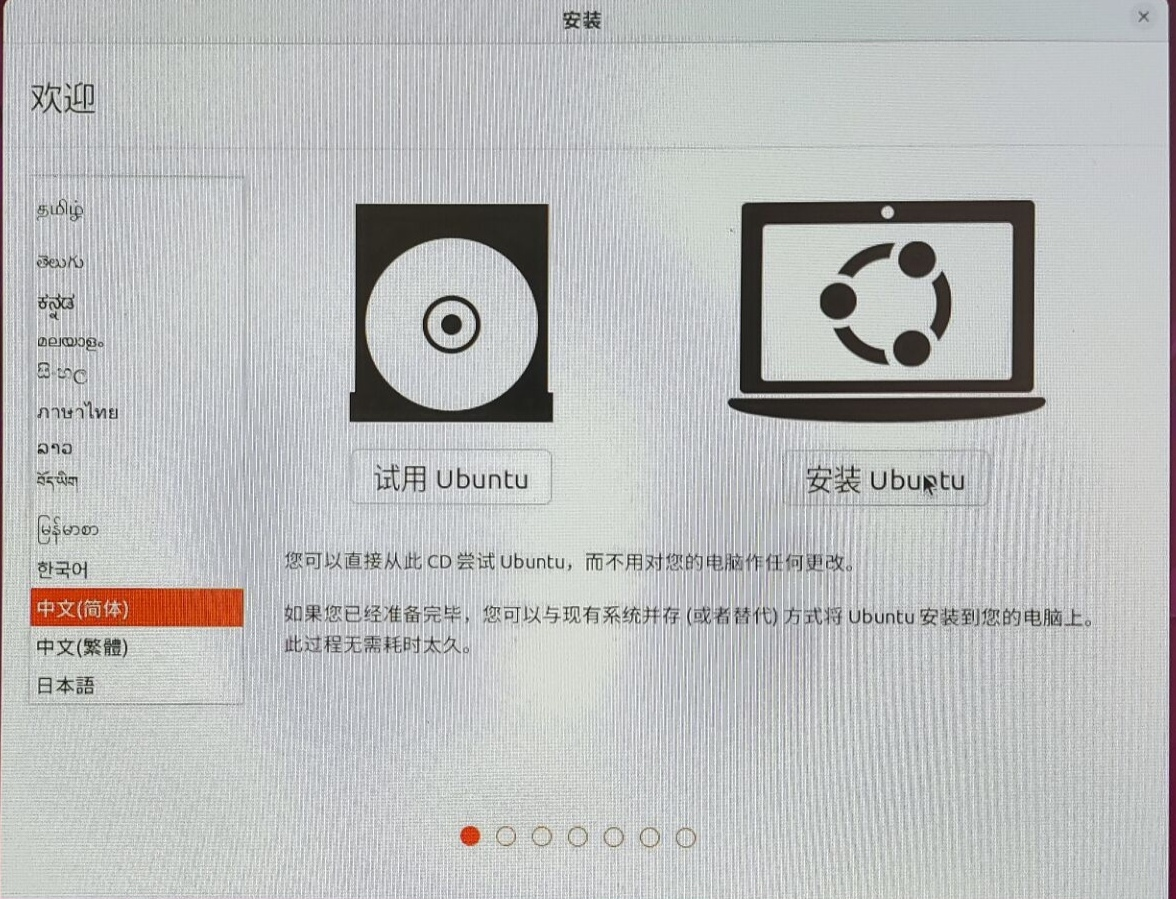
\includegraphics[width=0.7\textwidth]{install2.jpg}
    \caption{进入试用ubuntu界面} % 图片标题
\end{figure}

选择试用后我们会进入到ubuntu的主页面,打开终端,再次打开gparted

\begin{tcode}
    sudo apt-get install gparted
	sudo gparted
\end{tcode}

此时就可以对原来ubuntu系统的分区进行修改了,修改完点击确认等待扩容操作完成即可。

\subsection{系统数据备份}

恭喜你已经成功安装了ubuntu双系统,作为新手的你想来在刚刚的安装过程中一定是非常小心谨慎的,毕竟你也不想系统出现什么差错。在后续的工作中我们经常需要安装各种各样的安装包并对系统的环境进行配置,如果不小心配错了东西,重则系统可能无法正常工作(简称寄了)。这时候你就需要在启动页面进入“Ubuntu高级选项”对系统进行修复,或者直接重装系统。这是我们比较不愿意看到的情况,因此我们很有必要学习对系统的环境进行备份,这样即使环境配崩了也能恢复到配环境之前的状态,保留之前的工作。

\subsubsection{timeshift系统快照}

timeshift是linux上一款用于数据备份和恢复的软件,使用时会像相机一样给系统照个相。下面介绍一下timeshift的使用流程。

\textbf{安装timeshift}

\begin{tcode}
	sudo apt update
	sudo apt install timeshift
\end{tcode}

ubuntu也可以在软件中心直接搜索下载

\textbf{制作快照}

首先最好准备一个U盘,然后点击timeshift的图标启动,或者在终端输入

\begin{tcode}
	sudo timeshift-launcher
\end{tcode}

进入timeshift图形化操作界面,首先选择快照类型。RSYNC 是一种常见的文件同步协议,在 Timeshift 中用于增量式系统备份。备份时仅复制有改动的部分,因此通常比完整备份要小,创建速度更快。Btrfs 是一种支持快照等高级特性的文件系统。Timeshift 利用 Btrfs 的快照功能,可以创建系统的只读快照。这种类型的快照创建速度比 RSYNC 更快,占用的存储空间更小。但前提是,你的系统必须使用 Btrfs 文件系统。一般来说我们选择“RSYNC”。

备份位置最好选择在非系统硬盘或移动U盘,但要保证磁盘类型是ext4等linux类型。否则暂时选系统盘也行。选好盘后备份数据默认会保存在该硬盘下根目录下的 /timeshift 目录下。

备份时间有每月备份一次,每周备份一次、每日备份一次、每小时备份一次、每次开机备份一次,数字表示最多存几个快照,多了的话会删除最旧的那次快照。

“用户主目录”那栏根据自己需要的备份情况来选择,“筛选”那栏也是,可以选择添加所需目录或将其过滤。

\textbf{快照恢复}

如果系统损坏不大还可以正常使用,那么可以进入timeshift图形化界面,找到先前已经制作好的快照

\begin{figure}[H]
    \centering
    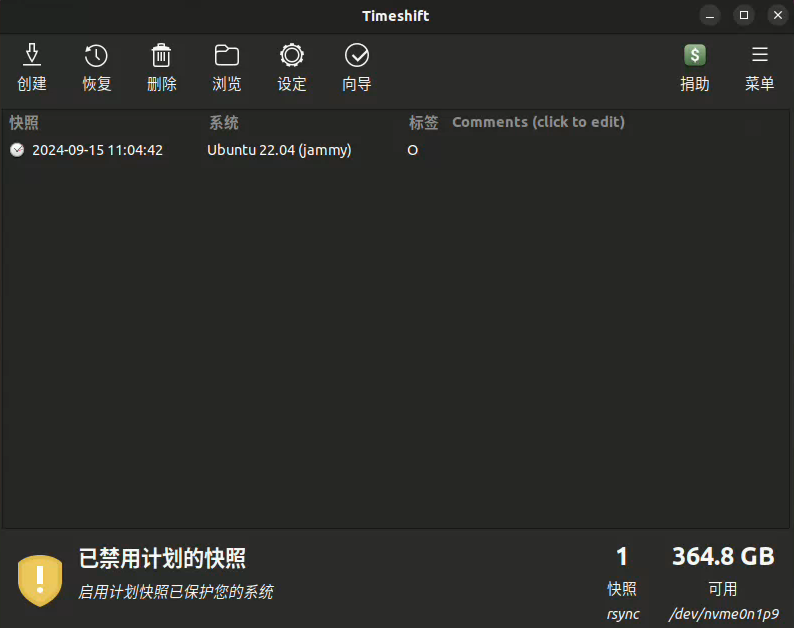
\includegraphics[width=0.7\textwidth]{restore1.png}
    \caption{timeshift图形化界面} % 图片标题
    \label{fig:restore1} % 图片标签,用于引用
\end{figure}

点击“恢复”,确认要恢复的目录后点击“下一步”即可进行恢复操作

\begin{figure}[H]
    \centering
    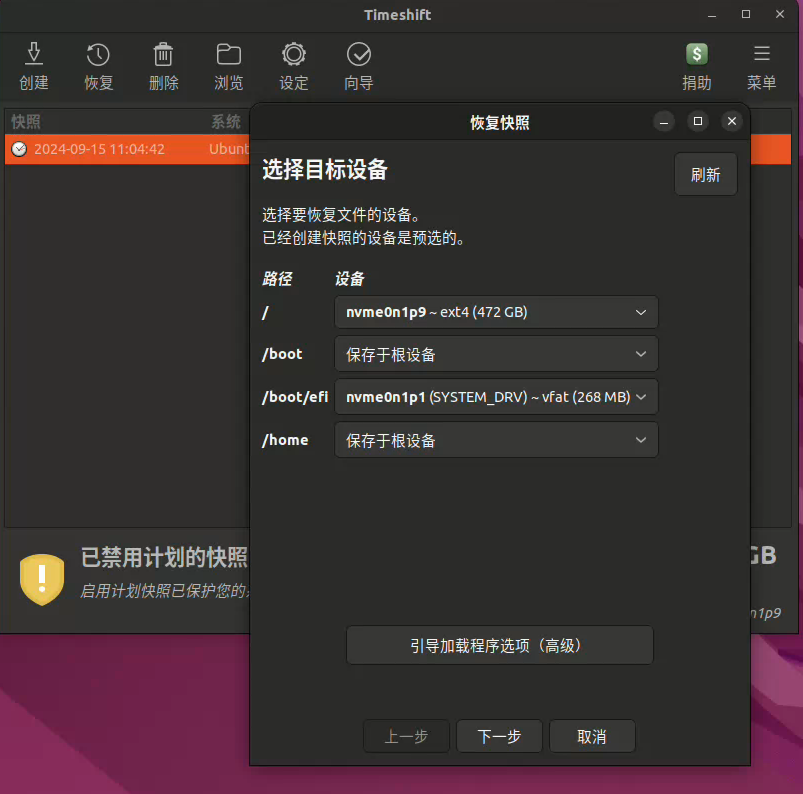
\includegraphics[width=0.7\textwidth]{restore2.png}
    \caption{timeshift快照恢复} % 图片标题
    \label{fig:restore2} % 图片标签,用于引用
\end{figure}

当然这个过程还可以通过命令行来完成:

备份快照

\begin{tcode}
	sudo timeshift --create --comments "快照名" --backup-device /dev/磁盘名
\end{tcode}

磁盘名可以通过 "fdisk -l" 或 "df -TH" 来查看

查看已存在的快照

\begin{tcode}
	sudo timeshift --list
\end{tcode}

选择上面已存在的其中一个快照进行恢复,如:快照'2024-07-01\_18-00-00'

\begin{tcode}
	sudo timeshift --restore --snapshot '2024-07-01_18-00-00' --skip-grub
\end{tcode}

如果已经无法加载图形化桌面,可以在开机时按“ctrl+alt+F1”(一般F1到F6都可以)进入tty终端,可以输入命令进行恢复。

如果连命令终端都进不去,只能通过启动盘再次进入安装ubuntu的页面,选择试用ubuntu,然后安装timeshift再进行恢复。

\subsubsection{系统镜像备份}

linux秉承着一切皆文件的思想,系统备份就相当于把整个根目录所有文件打包压缩保存。

\textbf{镜像制作}

备份前先切换到root用户,避免权限问题,然后切换到根目录,输入

\begin{tcode}
	tar -cvpzf /media/Disk/myDisk/ubuntu_backup@`date +%Y-%m+%d`.tar.gz --exclude=/proc --exclude=/tmp --exclude=/boot --exclude=/home --exclude=/lost+found --exclude=/media --exclude=/mnt --exclude=/run /
\end{tcode}

下面解释一下上面这条命令:tar就是一个打包命令,

\begin{tcode}
	/media/Disk/myDisk/ubuntu_backup@`date +%Y-%m+%d`.tar.gz
\end{tcode}

这个是备份文档的存放路径,myDisk表示你的移动硬盘名字,挂载在/media/Disk目录下,

\begin{tcode}
	ubuntu_backup@date +%Y-%m+%d.tar.gz
\end{tcode}

这是备份文件的名字,这里用了一个shell命令

\begin{tcode}
	date +%Y-%m+%d
\end{tcode}

用于记录备份时间。接下来看看–exclude参数中的内容。

假设现在ubuntu中有四个分区:/、/home、/boot、swap,其中/home、/boot两个分区出问题的概率很小,而且变动也不会太频繁,因此在定期备份时可以减小对这两个分区的备份频率。一般系统坏了都是/分区的问题,/home没什么关系。再来看看其他排除的目录:

/proc:一个虚拟文件系统,系统运行的每一个进程都会自动在这个目录下面创建一个进程目录。既然是系统自动创建,也就没必要备份的必要了。

/tmp:一个临时文件夹,系统的一些临时文件会放在这里。

/lost+found:系统发生错误时(比如非法关机),可以在这里找回一些丢失文件。

/media:多媒体挂载点,像u盘、移动硬盘、windons分区等都会自动挂载到这个目录下。

/mnt:临时挂载点,你可以自己挂载一些文件系统到这里。

/run:系统从启动以来产生的一些信息文件。

另外,有可能备份到最后系统会提示"tar: 由于前次错误,将以上次的错误状态退出",这个警告可以忽略,没什么影响的。

\textbf{镜像恢复}

这里有两种还原方式:

\begin{enumerate}
    \item 直接操作
    
    如果你系统出问题了,但是还可以进入终端,那就可以直接解压备份文件进行还原。切换到root,并且换到/根目录,打开终端,输入
    
    \begin{tcode}
        tar -xvpzf /media/Disk/myDisk/ubuntu_boot_backup@2016-6-6.tar.gz -C /
    \end{tcode}

    \item 使用启动盘还原
    
    如果你连系统都不能登录了,就要使用U盘启动盘进行还原了。依旧是先进入试用ubuntu界面,切换到root,打开终端,输入

    \begin{tcode}
        mkdir /mnt/sys
        mount /dev/sdaX /mnt/sys
        tar -xvpzf /media/myDisk/ubuntu_boot_backup@2016-6-6.tar.gz -C /mnt/sys
    \end{tcode}

    注意先创建一个临时目录用于挂载你的/根目录分区,sdaX代表你的/根目录分区,如果不知道就用fdisk -l查看一下,另外如果你的移动硬盘没有被自动挂载,你也需要手动创建一个临时目录进行挂载。

    因为 tar还原是只会覆盖相同的文件,但是这种方法只是恢复备份时的文件,就是说如果某些文件丢失或损坏了,这样可以恢复修复这些文件,但不能删除自备份到恢复前这期间所生成的其它文件,说白了就是假如你备份系统时有1234这四个文件,如果三天后,由于某些原因变成了1234’5(4改变了),你恢复后,就会变成12345,其中4’恢复成备份时的文件,5保留。
\end{enumerate}



\subsection{卸载重装ubuntu系统*}

如果你真的碰巧忘记备份镜像了,而你修改的环境变量又真的无法修复回去,或者有修复它的时间还不如重装一遍,那还是老老实实卸载重装吧。当然,希望各位自己永远不要用到这里的方法,在每次配环境前一定养成备份镜像的好习惯。

还是再提醒一下,重装之前备份好原ubuntu系统上的工作数据。

进入windows系统,右键“此电脑”选择“管理”,点击“磁盘管理”进入分区界面。确认好ubuntu系统存放的分区并将其删除,注意一定要将所有ubuntu分区都删除掉,不要错选到windows的分区!

搜索CMD(或搜索命令行),并用管理员身份打开。输入
\begin{tcode}
	diskpart
	list disk
\end{tcode}

确定windows系统的EFI分区,一般来说第一个磁盘0就是。输入
\begin{tcode}
	select disk 0
	list partition
\end{tcode}

然后确认ubuntu系统所在的分区,一般是在类型栏第一个显示为“系统”的分区,给该分区分配可见盘符,输入
\begin{tcode}
	select partition 2
	assign letter=F
\end{tcode}

这时候可以在电脑上看到一个磁盘F,但是没有权限访问。

再搜索记事本,用管理员权限打开,点击“文件”->“打开”->“磁盘F”,可以在打开界面看见F盘中的EFI文件夹,进入里面删掉ubuntu这个文件夹(该文件夹中内容无法访问但是可以直接删除)。删除后关闭记事本,在CMD中关闭刚刚分配的F盘,输入
\begin{tcode}
	remove letter=F
\end{tcode}

提示成功删除后ubuntu就已经完整的删除了,接下来就按照一开始安装ubuntu系统的步骤再重新安装一遍就可以了。

经实测发现,这里的方法会删除电脑中所有的ubuntu系统,如果你的电脑中有两个ubuntu系统那么还请慎用。



\subsection{linux系统的基本操作}

ubuntu系统为我们提供了完整的图形化界面,大部分操作已经可以通过图形化界面来完成,但如何通过命令行来和linux系统进行交互仍是基本功,下面我们就来简单介绍一下linux系统的基本操作。
\subsubsection{linux文件系统基本概念}
\textbf{linux目录结构}

首先我们来看一下linux系统的树状目录结构:

\begin{figure}[H]
    \centering
    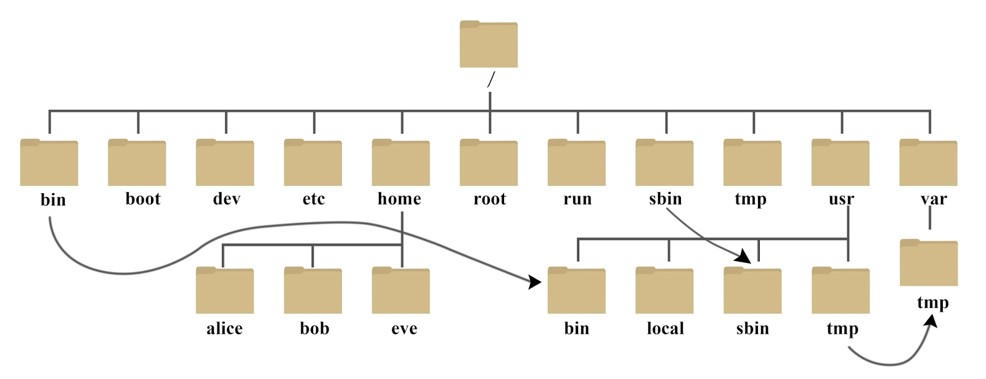
\includegraphics[width=0.9\textwidth]{linux7.jpg}
    \caption{linux系统树状目录结构} % 图片标题
    \label{fig:linux7} % 图片标签,用于引用
\end{figure}

可以看到整个linux系统是由若干个文件夹反复嵌套组成的,目录结构如同一棵倒置的树,因此最上面的文件夹被称为“根目录”。

\textbf{“一切皆文件”}

在linux系统中有一个非常重要的、区别于windows系统的概念是“一切皆文件”,也就是把一切资源都看作是文件,包括硬件设备(通常称为设备文件),这样好处是用户可以用读写文件的方式实现对硬件的访问。举个简单的例子:假如现在将U盘插到电脑上,在windows上会看到出现一个新的磁盘,在linux中则可以在/dev目录下找到新出现的文件夹,该文件夹中就存放了插入U盘的相关内容,用户不仅可以修改U盘中存储的文件,还可以修改其相关配置。

\textbf{挂载}

在上述例子中,U盘与linux系统建立连接的过程称为“挂载”。Linux系统中没有磁盘分区的逻辑概念,任何一个种类的文件系统被创建后,都需要挂载到某个特定的目录才能使用,这个过程相当于激活一个文件系统,使它能够使用。简单来说“挂载”就是将linux本身文件目录与硬件设备的文件目录合二为一,下图中展示了一个简单的挂载实例。

\begin{figure}[H]
    \centering
    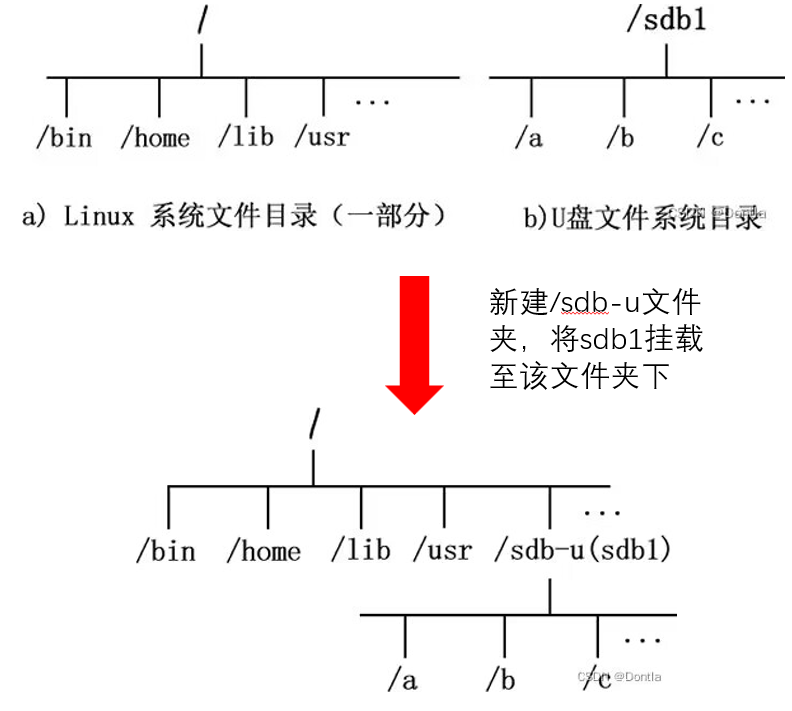
\includegraphics[width=0.7\textwidth]{linux8.png}
    \caption{挂载实例} % 图片标题
    \label{fig:linux8} % 图片标签,用于引用
\end{figure}

Windows的文件系统挂载使用其内部机制完成,用户基本无法探知其过程。而Linux使用mount工具对文件系统进行挂载。挂载文件系统时,需要明确挂载点,在创建文件系统后,操作系统会提示将此文件系统挂载至哪个位置,这个位置就是挂载点,通常选择“/”即根目录。挂载操作在备份系统镜像时经常用到。

\textbf{主要文件夹及其作用}

/bin:bin 是 Binaries (二进制文件) 的缩写, 这个目录存放着最经常使用的命令。

/boot:这里存放的是启动 Linux 时使用的一些核心文件,包括一些连接文件以及镜像文件。

/dev:dev 是 Device(设备) 的缩写, 该目录下存放的是 Linux 的外部设备,在 Linux 中访问设备的方式和访问文件的方式是相同的。

/etc:etc 是 Etcetera(等等) 的缩写,这个目录用来存放所有的系统管理所需要的配置文件和子目录。

/home:用户的主目录,在 Linux 中,每个用户都有一个自己的目录,一般该目录名是以用户的账号命名的,如上图中的 alice、bob 和 eve。

/lib:lib 是 Library(库) 的缩写这个目录里存放着系统最基本的动态连接共享库,其作用类似于 Windows 里的 DLL 文件。几乎所有的应用程序都需要用到这些共享库。

/opt:opt 是 optional(可选) 的缩写,这是给主机额外安装软件所摆放的目录。比如你安装一个ORACLE数据库则就可以放到这个目录下。默认是空的。

/root:该目录为系统管理员,也称作超级权限者的用户主目录。

/usr:usr 是 unix system resources(unix 系统资源) 的缩写,这是一个非常重要的目录,用户的很多应用程序和文件都放在这个目录下,类似于 windows 下的 program files 目录。

/var:var 是 variable(变量) 的缩写,这个目录中存放着在不断扩充着的东西,我们习惯将那些经常被修改的目录放在这个目录下。包括各种日志文件。

在这些文件夹中,/bin,/etc,/usr,/var内存放着重要的系统文件,如果删除可能会导致系统出错,因此在平时操作时要多加注意。

\subsubsection{linux系统基本操作}
由于篇幅有限,本部分仅能列出平时操作中最常用的部分,其它内容如需用到请读者自行查阅资料。

\textbf{01用户管理}
\begin{table}[!htbp]
	\centering
	\begin{tabular}{cc}
		\toprule[1.5pt]
		命令 & 作用\\
		\midrule[1pt]
		$id \enspace [name]$			&查看用户UID和GID信息\\
		$who$			&查看当前所有登录的用户列表\\
		$whoami$			&查看当前登录用户的账户名\\
		$su \enspace -[name]$			&切换用户,并且切换目录\\
		$exit$			&退出当前登录用户\\
		$passwd\enspace [name]$			&设置用户密码\\
		\bottomrule[1.5pt]
	\end{tabular}
\end{table}

说明:
\begin{enumerate}
	\item -\enspace 可以切换到用户家目录,否则保持位置不变
	\item su 不接用户名,可以切换到 root 
	\item 命令前加sudo:以超级用户权限运行命令
\end{enumerate}

\textbf{02系统信息}

\begin{table}[!htbp]
	\centering
	\begin{tabular}{cc}
		\toprule[1.5pt]
		语法 & 作用\\
		\midrule[1pt]
		$free\enspace -m$			&以MB为单位显示系统内存使用情况\\
		$uname \enspace -amnrsv \enspace --help \enspace --version$			&显示电脑以及操作系统的相关信息\\
		\bottomrule[1.5pt]
	\end{tabular}
\end{table}

\begin{center}
\textbf{uname参数说明}

	\begin{tabular}{cc}
		\toprule[1.5pt]
		参数 & 作用\\
		\midrule[1pt]
		$-a\enspace --all$		&显示全部的信息\\
		$-m\enspace --machine $		&显示处理器类型\\
		$-n\enspace --nodename $		&显示主机名\\
		$-r\enspace --release $		&显示内核版本号\\
		$-s\enspace --sysname $		&显示操作系统名称\\
		$-v $		&显示操作系统的版本\\
		$--help $		&显示帮助\\
		$--version $		&显示版本信息\\
		$-p $		&显示处理器类型(与 -m 选项相同)\\
		\bottomrule[1.5pt]
	\end{tabular}
\end{center}

\textbf{03软件安装}

软件安装命令有yum,apt等等,比较常用的是apt,apt 命令执行需要超级管理员权限

\begin{table}[!htbp]
	\centering
	\begin{tabular}{cc}
		\toprule[1.5pt]
		语法 & 作用\\
		\midrule[1pt]
		$  apt\enspace [options] \enspace [command] \enspace [package ...]$		&查找、安装、升级、删除软件包\\
		\bottomrule[1.5pt]
	\end{tabular}
\end{table}

\textbf{options}:可选,选项包括 -h(帮助),-y(当安装过程提示选择全部为"yes"),-q(不显示安装的过程)等等

\textbf{command}:要进行的操作

\textbf{package}:安装的包名\\

\begin{center}
\textbf{apt常用命令如下}

	\begin{tabular}{cc}
		\toprule[1.5pt]
		命令 & 作用\\
		\midrule[1pt]
		$  apt\enspace update$	&列出所有可更新的软件清单\\
		$  apt\enspace upgrade$	&升级软件包\\
		$  apt\enspace list \enspace --upgradable$		&列出可更新的软件包及版本信息\\
		$  apt\enspace full-upgrade$	&升级软件包前先删除需要更新软件包\\
		$  apt\enspace install \enspace \textless package1\textgreater \enspace \textless package2\textgreater $	&安装指定的软件\\
		$  apt\enspace update \enspace \textless package\textgreater $		&更新指定的软件\\
		$  apt\enspace show \enspace \textless package\textgreater $	&显示软件包具体信息\\
		$  apt\enspace remove \enspace \textless package\textgreater $		&删除软件包\\
		$  apt\enspace autoremove$		&清理不再使用的依赖和库文件\\
		$  apt\enspace purge \textless package\textgreater $		&移除软件包及配置文件\\
		$  apt\enspace search \enspace \textless keyword\textgreater $		&找软件包命令\\
		$  apt\enspace list \enspace --installed$		&列出所有已安装的包\\
		$  apt\enspace list \enspace --all-versions$	&列出所有已安装的包的版本信息\\
		\bottomrule[1.5pt]
	\end{tabular}
\end{center}

\textbf{04文件与目录管理}

首先先介绍一些常用概念

\begin{enumerate}
\item 绝对路径:路径的写法,由根目录\enspace /\enspace 写起,例如:/usr/share/doc 这个目录。
\item 相对路径:路径的写法,相对于当前所处的文件夹位置,不是由\enspace /\enspace 写起,例如由 /usr/share/doc 要到 /usr/share/man 底下时,可以写成:cd man
\item \enspace .\enspace :在相对路径中使用,表示当前目录
\item \enspace ..\enspace :在相对路径中使用,表示上一级目录
\item \enspace *\enspace :通配符,可以代表文件名中的任意字符或字符串,但不能与句点打头的文件名匹配
\item 文件类型:分为目录(d),文件(-),链接文件(l),装置文件里可供储存的接口设备(b),装置文件里面的串行端口设备(c)
\item 文件基本属性:分为可读(r),可写(w),可执行(x)。Linux文件属性有两种设置方法,一种是数字,一种是符号。使用数字来代表各个权限时,各权限的分数对照为:r:4,w:2,x:1
\end{enumerate}

处理文件和目录的命令有很多,这里分表整理了一些常用命令的语法及其选项和参数仅供大家参考

\begin{center}
\textbf{常用处理文件和目录的命令}

	\begin{tabular}{cc}
		\toprule[1.5pt]
		语法 & 作用\\
		\midrule[1pt]
		$  ls$		&列出当前目录中的文件和子目录\\
		$  pwd$		&显示当前工作目录的路径\\
		$  cd\enspace /path/to/directory$		&切换工作目录\\
		$  mkdir\enspace [directory]$		&创建新目录\\
		$  cp\enspace [source]\enspace [destination]$		&复制文件或目录\\
		$  rm\enspace [file name]$		&删除文件或目录\\
		$  mv\enspace [old]\enspace [new]$		&移动或重命名文件或目录\\
		$  chmod\enspace [permissions]\enspace [file name]$		&修改文件或目录的权限\\
		$  tar\enspace [options]\enspace -f\enspace archive.tar\enspace [files...]$	&解压或压缩文件或目录\\
		$  zip\enspace [options]\enspace output.zip\enspace [files...]$		&压缩文件或目录\\
		$ unzip archive.zip$		&解压文件或目录\\
		\bottomrule[1.5pt]
	\end{tabular}
\end{center}

\begin{center}
\textbf{ls\enspace 选项和参数}

	\begin{tabular}{cc}
		\toprule[1.5pt]
		参数 & 作用\\
		\midrule[1pt]
		$  -a $		&列出当前目录中全部的文件,包括隐藏文件\\
		$  -d $		&仅列出目录本身,而不是列出目录内的文件数据\\
		$  -l $		&长数据串列出,包含文件的属性与权限等\\
		\bottomrule[1.5pt]
	\end{tabular}
\end{center}

\begin{center}
\textbf{mkdir\enspace 选项和参数}

	\begin{tabular}{cc}
		\toprule[1.5pt]
		参数 & 作用\\
		\midrule[1pt]
		$  -m $		&配置文件的权限\\
		$  -p $		&递归创建所需目录\\
		\bottomrule[1.5pt]
	\end{tabular}
\end{center}

\begin{center}
\textbf{cp\enspace 选项和参数}

	\begin{tabular}{cc}
		\toprule[1.5pt]
		参数 & 作用\\
		\midrule[1pt]
		$  -a $		&相当于\enspace -pdr\enspace 的意思\\
		$  -d $		&若来源档为链接档的属性(link file),则复制链接档属性而非文件本身\\
		$  -f $		&强制,若目标文件已经存在且无法开启,则移除后再尝试一次\\
		$  -i $		&若目标文件或目录已经存在,在覆盖时会先询问用户\\
		$  -l $		&进行硬式链接的链接档创建,而非复制文件本身\\
		$  -p $		&连同文件的属性一起复制过去,而非使用默认属性(备份常用)\\
		$  -r $		&递归持续复制,用于目录的复制(常用)\\
		$  -s $		&复制成为符号链接档,即“捷径”文件\\
		$  -u $		&若 destination 比 source 旧才升级 destination\\
		\bottomrule[1.5pt]
	\end{tabular}
\end{center}

\begin{center}
\textbf{rm\enspace 选项和参数}

	\begin{tabular}{cc}
		\toprule[1.5pt]
		参数 & 作用\\
		\midrule[1pt]
		$  -f $		&强制的意思,如果目标文件已经存在,不会询问而直接覆盖\\
		$  -i $		&互动模式,在删除前会询问使用者是否动作\\
		$  -r $		&递归删除,常用在目录的删除\\
		\bottomrule[1.5pt]
	\end{tabular}
\end{center}

\begin{center}
\textbf{mv\enspace 选项和参数}

	\begin{tabular}{cc}
		\toprule[1.5pt]
		参数 & 作用\\
		\midrule[1pt]
		$  -f $		&强制的意思,如果目标文件已经存在,不会询问而直接覆盖\\
		$  -i $		&若目标文件已经存在时,会询问是否覆盖\\
		$  -u $		&若目标文件已经存在,且 source 比较新,才会升级 \\
		\bottomrule[1.5pt]
	\end{tabular}
\end{center}

\begin{center}
\textbf{chmod\enspace 选项和参数}

	\begin{tabular}{cc}
		\toprule[1.5pt]
		参数 & 作用\\
		\midrule[1pt]
		$  -R $		&进行递归的持续变更,连同次目录下的所有文件都会变更\\
		$  u $		&user,用户身份\\
		$  g $		&group,组 \\
		$  o $		&others,其他身份 \\
		$  a $		&all,全部的身份 \\
		$  +\enspace -\enspace = $		&对权限加入,除去,设定 \\
		\bottomrule[1.5pt]
	\end{tabular}
\end{center}

使用chmod命令修改文件或目录权限有两种方式,一是用权限数字更改,方法为:

chmod [-R] xyz 文件或目录

其中xyz就是刚刚提到的数字类型的权限属性,为 rwx 属性数值的相加。

第二种是用符号类型改变文件权限,方法为:

chmod\enspace ([身份])\enspace +/-/=\enspace [permissions]\enspace [file name]

举例:

chmod 777 filename    修改文件/目录权限为所有人可读可写可执行

chmod u+x ex1.py        为 ex1.py 文件拥有者增加可执行权限

\begin{center}
\textbf{tar\enspace 选项和参数}

	\begin{tabular}{cc}
		\toprule[1.5pt]
		参数 & 作用\\
		\midrule[1pt]
		$  -f\enspace archive.tar $		&指定归档文件的名称\\
		$  -c $		&创建新的归档文件\\
		$  -v $		&显示详细输出,列出被添加/解压到归档中的文件 \\
		$  -f $		&指定归档文件的名称 \\
		$  -x $		&解压归档文件 \\
		$  -z $		&使用 gzip 压缩归档文件 \\
		$  -r $		&向已存在的归档中追加文件 \\
		\bottomrule[1.5pt]
	\end{tabular}
\end{center}

tar命令的参数繁多,此处只列举了以上最最常见的参数。

\begin{center}
\textbf{zip\enspace 选项和参数}

	\begin{tabular}{cc}
		\toprule[1.5pt]
		参数 & 作用\\
		\midrule[1pt]
		$  -r $		&递归压缩目录及其子目录中的所有文件\\
		$  -e $		&为压缩文件设置密码保护\\
		$  -q $		&静默模式,不显示压缩过程 \\
		$  -v $		&显示详细的压缩过程 \\
		$  -x $		&排除某些文件或目录,不进行压缩 \\
		$  -m $		&压缩后删除原始文件 \\
		$  -0\enspace \texttildelow \enspace -9 $		&指定压缩级别,-0 表示存储不压缩,-9 表示最高压缩率,默认是 -6 \\
		\bottomrule[1.5pt]
	\end{tabular}
\end{center}

\textbf{05查找、管道与重定向}

\begin{center}
\textbf{grep\enspace 的语法}

	\begin{tabular}{cc}
		\toprule[1.5pt]
		语法 & 作用\\
		\midrule[1pt]
		$  grep\enspace [option]\enspace pattern\enspace [files]$		&查找文件里符合条件的字符串或正则表达式\\
		\bottomrule[1.5pt]
	\end{tabular}
\end{center}

\textbf{pattern}:表示要查找的字符串或正则表达式

\textbf{files}:要查找的文件名,可以同时查找多个文件,如果省略 files 参数,则默认从标准输入中读取数据\\

重定向是一种强大的功能,它允许用户改变命令的输入或输出方向,从而更灵活地控制数据流。重定向主要包括三种类型:标准输入重定向(stdin)、标准输出重定向(stdout)和标准错误输出重定向(stderr)。

\begin{center}
\textbf{重定向}

	\begin{tabular}{ccc}
		\toprule[1.5pt]
		输入输出 & 重定向 & 意义\\
		\midrule[1pt]
		$  stdin$		& <\enspace /\enspace <<		& <重定向到文件中去读取,<<表示结束输入的字符\\
		$  stdout$		& >\enspace /\enspace >>		& >会覆盖文件原有内容,>>则会在文件末尾追加内容\\
		$  stderr$		& 2>\enspace /\enspace 2>>		&作用与标准输出重定向类似,但专门用于处理错误信息\\
		\bottomrule[1.5pt]
	\end{tabular}
\end{center}

管道符|主要用于多重命令处理,前面命令的打印结果作为后面命令的输入,不过其只能重定向stdout即成功执行的命令

管道符常和grep结合使用用于过滤信息,列出所查找关键字所在的位置

\begin{center}
\textbf{grep的参数}

	\begin{tabular}{cc}
		\toprule[1.5pt]
		参数 & 作用\\
		\midrule[1pt]
		$  -i$		&忽略大小写进行匹配\\
		$  -v$		&反向查找,只打印不匹配的行\\
		$  -n$		&显示匹配行的行号\\
		$  -r$		&递归查找子目录中的文件\\
		$  -l$		&只打印匹配的文件名\\
		$  -c$		&只打印匹配的行数\\
		\bottomrule[1.5pt]
	\end{tabular}
\end{center}

\textbf{06文件内容}

\begin{center}
\textbf{文件内容操作}

	\begin{tabular}{cc}
		\toprule[1.5pt]
		语法 & 作用\\
		\midrule[1pt]
		$  cat [file name]    $		&由第一行开始显示文件内容(只读)\\
		$  touch [file name]    $		&创建空文件或更新文件的时间戳\\
		$  gedit [file name]    $		&创建空文件或更改文件内容\\
		$  vim/vi [file name]    $		&创建空文件或编辑文件内容\\
		\bottomrule[1.5pt]
	\end{tabular}
\end{center}

在所有关于文件内容的操作中,这里着重介绍一下vim。vim是从 vi 发展出来的一个文本编辑器。代码补全、编译及错误跳转等方便编程的功能特别丰富。

vi/vim 共分为三种模式,命令模式、输入模式和命令行模式

\textbf{命令模式}:用户刚刚启动 vi/vim,便进入了命令模式。此状态下敲击键盘动作会被 vim 识别为命令,而非输入字符,比如我们此时按下i,并不会输入一个字符,i被当作了一个命令。

\begin{center}
\textbf{命令模式常用操作}

	\begin{tabular}{cc}
		\toprule[1.5pt]
		命令 & 作用\\
		\midrule[1pt]
		$  i    $		&切换到输入模式,在光标当前位置开始输入文本\\
		$  x    $		&删除当前光标所在处的字符\\
		$  :    $		&切换到底线命令模式,以在最底一行输入命令\\
		$  a    $		&进入插入模式,在光标下一个位置开始输入文本\\
		$  o    $		&在当前行的下方插入一个新行,并进入插入模式\\
		$  O    $		&在当前行的上方插入一个新行,并进入插入模式\\
		$  dd    $		&剪切当前行\\
		$  yy    $		&复制当前行\\
		$  p    $		&粘贴剪贴板内容到光标下方\\
		$  P    $		&粘贴剪贴板内容到光标上方\\
		$  u    $		&撤销上一次操作\\
		$  Ctrl + r    $		&重做上一次撤销的操作\\
		\bottomrule[1.5pt]
	\end{tabular}
\end{center}

\textbf{输入模式}:在此状态下敲击键盘会被vim识别为输入内容,同时也有一些按键命令。

\begin{center}
\textbf{输入模式常用操作}

	\begin{tabular}{cc}
		\toprule[1.5pt]
		命令 & 作用\\
		\midrule[1pt]
		$  keyboard+Shift    $		&输入字符\\
		$  ENTER    $		&回车键,换行\\
		$  BACK SPACE    $		&退格键,删除光标前一个字符\\
		$  DEL    $		&删除键,删除光标后一个字符\\
		$  Arrow keys    $		&在文本中移动光标\\
		$  HOME/END    $		&移动光标到行首/行尾\\
		$  Page Up/Page Down    $		&上/下翻页\\
		$  Insert    $		&切换光标为输入/替换模式,光标将变成竖线/下划线\\
		$  ESC    $		&退出输入模式,切换到命令模式\\
		\bottomrule[1.5pt]
	\end{tabular}
\end{center}

\textbf{底线命令模式}:在命令模式下按下 :(英文冒号)就进入了底线命令模式。

\begin{center}
\textbf{底线模式基本命令}

	\begin{tabular}{cc}
		\toprule[1.5pt]
		命令 & 作用\\
		\midrule[1pt]
		$  :w    $		&保存文件\\
		$  :q    $		&退出vim编辑器\\
		$  :wq    $		&保存文件并退出vim编辑器\\
		$  :q!    $		&强制退出vim编辑器,并不保存修改\\
		$  :qa!    $		&强制退出vim编辑器,并不保存修改\\
		\bottomrule[1.5pt]
	\end{tabular}
\end{center}

以上就是linux系统中关于文件和目录的基本操作,俗话说熟能生巧,请读者利用空余时间多加练习,尽快适应linux系统的命令行操作。

\subsection{简单的shell脚本和环境变量}

\subsubsection{shell简介}

在windows系统中,我们使用电脑主要是通过图形化界面点击某个图标来启动某个程序;在linux系统中我们更频繁的使用终端和命令行。然而这些都只是我们控制计算机的表象,真正能够控制计算机硬件(CPU、内存、显示器等)的只有操作系统内核(Kernel),图形界面和命令行只是架设在用户和内核之间的一座桥梁。

考虑到安全等原因,用户不能直接接触内核,因此需要另外再开发一个程序,让用户通过使用这个程序来间接地与内核进行交互。该程序的作用就是接收用户的操作(点击图标、输入命令),并进行简单的处理,然后再传递给内核。用户界面和命令行就是这个另外开发的程序,在 Linux下,这个命令行程序叫做 shell 。

\begin{figure}[H]
    \centering
    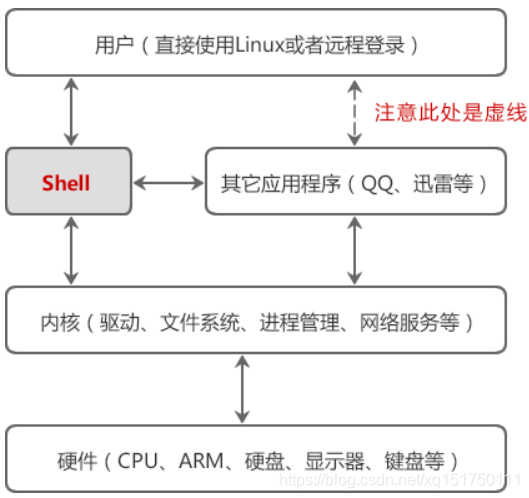
\includegraphics[width=0.7\textwidth]{shell.png}
    \caption{shell工作流程示意图} % 图片标题
    \label{fig:shell} % 图片标签,用于引用
\end{figure}

shell的一大特性就是它是一个应用程序,它连接了用户和 Linux 内核,让用户能够更加高效、安全、低成本地使用 Linux 内核。另一大特性是它是一个命令语言解释器,shell把我们在计算机上的操作或我们的命令,翻译为计算机可识别的二进制命令,传递给内核,以便调用计算机硬件执行相关的操作;计算机执行完命令后,再通过Shell翻译成自然语言,呈现在我们面前。同时,Shell 程序设计语言支持在高级语言里所能见到的绝大多数程序控制结构,比如循环,函数,变量和数组等等。

常见的shell有Bourne shell (sh), C shell (csh), Korn shell (ksh), Bourne Again shell(bash, sh 的扩展),zsh等等。

启动shell的方法有两种,一是进入linux控制台,二是使用终端(快捷键为ctrl+alt+t)

\subsubsection{简单的shell脚本}

shell

\textbf{新建一个shell脚本}

打开文本编辑器,新建一个文件 test.sh

\begin{tcode}
	vim test.sh
\end{tcode}

然后在shell脚本的第一行输入

\begin{tcode}
	#!/bin/bash
\end{tcode}

\#! 是一个约定的标记,它告诉系统这个脚本需要什么解释器来执行,即使用哪一种 shell。在第一行下面就可以用shell编程语言输入脚本内容了,以下是一个简单的例子:

\begin{tcode}
	#!/bin/bash
	echo "Hello World !"
\end{tcode}

shell脚本可用于ROS程序自启,即编写一系列命令行操作,启动程序时无需打开终端敲命令行,只需启动一个shell脚本即可。

\textbf{运行shell脚本}

运行shell脚本也有两种方式:

\begin{enumerate}
\item 作为可执行程序

先使脚本具有执行权限

\begin{tcode}
	chmod +x ./test.sh
\end{tcode}

再执行脚本

\begin{tcode}
	./test.sh
\end{tcode}

\item 作为解释器参数

直接运行解释器,其参数就是 shell 脚本的文件名。eg:

\begin{tcode}
	/bin/sh test.sh
	/bin/php test.php
\end{tcode}

这种方式运行的脚本,不需要在第一行指定解释器信息,写了也没用
\end{enumerate}

\subsubsection{linux中的bash}

根据刚刚对shell的介绍可以知道bash也是一种shell,事实上在大多数的linux系统中,bash是默认的缺省shell。当然如果你不想用bash也可以换成其他的shell(比如zsh也很好用)。

bash和shell一样有许多强大的功能,经常用到的有命令补全,通配符,命令历史记录,重定向,管道等等。bash的配置文件分为全局配置文件和个人配置文件:

\begin{center}
\textbf{bash主要文件}
	\begin{tabular}{cc}
		\toprule[1.5pt]
		文件 & 作用\\
		\midrule[1pt]
		$  /etc/profile    $		&系统的主配置文件,用于设置系统范围内的环境变量和其他系统的设置\\
		$  \texttildelow /.bashrc    $		&用于定义用户的命令别名和本地变量\\
		$  \texttildelow /.bash\_profile   $		&用于定义用户的环境变量,运行命令或脚本\\
		\bottomrule[1.5pt]
	\end{tabular}
\end{center}

其中我们会经常对.bashrc文件进行操作。

.bashrc是终端里面指令运行的配置脚本,是系统的隐藏文件,存放在\texttildelow 目录下。.bashrc的功能主要有两个:

\begin{enumerate}
\item 个性化指令alias:alias [指令别名]='原指令'

注意alias和=之间不能有空格

\item 设定环境路径:export PATH=\$PATH:路径
\end{enumerate}

对.bashrc中的内容进行修改后,在下一次打开新终端时修改内容才会生效,或执行source \texttildelow /.bashrc立刻生效。

\subsubsection{linux系统环境变量简介}

linux系统中有非常多的环境变量在控制系统的运行,常用的有:

\begin{enumerate}
\item PATH:决定了shell将到哪些目录中寻找命令或程序

\item HOME:当前用户主目录

\item SHELL:当前用户Shell类型
\end{enumerate}

这里我们主要介绍PATH环境变量

PATH说简单点就是一个字符串变量,当输入命令的时候linux会去查找PATH里面记录的路径,path 配置的路径下的文件可以在任何位置执行,并且可以通过which 可执行文件命令来找到该文件的位置。注意PATH是大写,linux中区分大小写。

我们先来查看一下PATH:

\begin{tcode}
	echo $PATH
\end{tcode}

终端中会输出

/usr/local/sbin:/usr/local/bin:/usr/sbin:/usr/bin:/sbin:/bin:/usr/games:

/usr/local/games:/usr/lib/wsl/lib:/snap/bin


每个路径中间用:隔开,输入命令时系统根据这些路径来寻找对应的可执行文件,先找到谁就用谁

设置环境变量的方法有两种:

\begin{enumerate}
\item export PATH=/bin:/sbin:/usr/bin:/usr/sbin

\item PATH="/bin:/sbin:/usr/bin:/usr/sbin"
\end{enumerate}

这两种方法都是将PATH环境变量设置为包含了/bin、/sbin、/usr/bin、/usr/sbin这四个目录,但不同在于第一个命令是将PATH变量设置为一个新的字符串,第二个命令则是将PATH变量设置为一个已经存在的字符串,会覆盖之前的设置。并且不用export设置的环境变量仅对当前shell起作用,不会传导到子进程,export设置的环境变量在子进程也有效,因此我们常用export命令来设置PATH环境变量。

修改环境变量的方法有三种:

\begin{enumerate}
\item 直接在终端输入

\begin{tcode}
	export PATH=/usr/local/mongodb/bin:$PATH
\end{tcode}

\$PATH表示在原有PATH的基础上继续在前面或后面添加相应路径,这样可以避免修改原有路径。由于是在终端中输入命令,因此这种修改方式仅对当前用户当前终端有效。

\item 修改.bashrc文件:在.bashrc文件中添加export PATH=/usr/local/mongodb/bin:\$PATH一行,保存退出后source或打开新终端即可生效。该方法对当前用户永久有效。

\item 修改/etc/profile文件:找到设置PATH的行,添加export PATH=/usr/local/mongodb/bin:\$PATH,系统重启或运行source /etc/profile后生效。由于是修改了整个系统的配置文件,因此该方法对所有用户永久有效。
\end{enumerate}

环境变量这里介绍的很浅,主要目的是让读者先对环境变量这个概念有所了解,在后续自己配环境的过程中逐步加深对环境变量的理解,避免对系统环境变量的误操作。



\subsection{git工具的使用}

\subsubsection{git简介}

git 是一个开源的分布式版本控制系统,用于敏捷高效地处理任何或小或大的项目,它可以在任何时间点,将文档的状态作为更新记录保存起来,也可以在任何时间点,将更新记录恢复回来。Git可以帮我们做到很多事情,比如代码的版本控制,分支管理,也提供了便于多人合作的平台。

在linux上安装git

\begin{tcode}
	sudo apt install git
\end{tcode}

\subsubsection{git基本概念}

在git中有一些比较重要的基本概念:

\textbf{本地仓库}:对本地代码进行管理的仓库,会包含代码的所有历史版本。

\textbf{远程仓库}:在开发者可以访问的网络内的某个服务器上有一个包含所有版本的仓库。

开发者可以把本地的新版本推送到远程仓库上,也可以把远程仓库上的新版本拉取到本地仓库上。由此可见,远程仓库为不同开发者之间的协作提供了一个渠道。

\textbf{工作区}:在本地计算机上的项目目录,你在这里进行文件的创建、修改和删除操作。工作区包含了当前项目的所有文件和子目录。

\textbf{暂存区}:临时存储区域,它包含了即将被提交到版本库中的文件快照。

\textbf{版本库}:包含项目的所有版本历史记录,每次提交都会在版本库中创建一个新的快照,这些快照是不可变的,确保了项目的完整历史记录。

\textbf{分支}:简单来说就是同一棵树上的两个分叉,实际上是指向更改快照的指针。

\textbf{暂存}:添加文件到暂存区准备提交。

\textbf{提交}:提交暂存区中的内容到本地仓库。

\textbf{推送}:推送本地仓库中的内容到远程仓库。

\textbf{克隆}:从远程仓库下载代码到本地的过程。

\textbf{合并}:假设分支A和分支B是从节点P分叉出来的,合并之后分支A和分支B会在一个新的节点后会和。

\textbf{变基}:从节点P开始,把分支A中各个节点按提交的顺序加在分支B的上面,因为一个节点对应一次内容改变,所以分支A中不想要的改变可以在变基的过程中跳过相应的节点。变基其实也可以理解成是另一种合并,只不过他的合并会让提交历史更为干净清晰。

\textbf{子模块}:将一个 git 仓库作为另一个 git 仓库的子目录。它能让你将另一个仓库克隆到自己的项目中,同时还保持提交的独立。

\subsubsection{git基本配置}

git 提供了一个叫做 git config 的命令,用来配置或读取相应的工作环境变量。这些环境变量,决定了 Git 在各个环节的具体工作方式和行为。这些变量可以存放在以下三个不同的地方:

\begin{enumerate}
\item /etc/gitconfig 文件:系统中对所有用户都普遍适用的配置。若使用 git config 时用 --system 选项,读写的就是这个文件。

\item \texttildelow /.gitconfig 文件:用户目录下的配置文件只适用于该用户。若使用 git config 时用 --global 选项,读写的就是这个文件。

\item 当前项目的 Git 目录中的配置文件(也就是工作目录中的 .git/config 文件):这里的配置仅仅针对当前项目有效。每一个级别的配置都会覆盖上层的相同配置,所以 .git/config 里的配置会覆盖 /etc/gitconfig 中的同名变量。
\end{enumerate}

\textbf{配置用户信息(个人访问令牌)}

github已经弃用了原先用个人用户名称和电子邮件地址来在每次提交代码时记录提交者的信息的方案,改用个人访问令牌。配置个人访问令牌的方法如下:

\begin{enumerate}
\item 在github设置界面点击进入“Developer settings”,访问 Personal Access Tokens中的Tokens(classic)页面
\item 点击 “Generate new token”,选择“Generate new token(classic)”
\item 为令牌选择一个描述性名称,选择 repo 权限,点击 “Generate token” 生成令牌,复制生成的令牌
\item 在提交代码时,当提示输入用户名和密码时,输入你的 GitHub 用户名和新生成的个人访问令牌即可
\end{enumerate}

\textbf{配置ssh密钥}

克隆github上的私人仓库不能使用https协议,只能使用SSH协议进行克隆,因此想要正常使用github还需要配置SSH密钥,具体方法如下:

\begin{enumerate}
\item 生成SSH密钥

\begin{tcode}
	ssh-keygen
\end{tcode}

生成后可在\texttildelow 目录下找到.ssh文件夹
\item 进入.ssh文件夹,复制其中id\_rsa.pub文件中的内容
\item 在github中进入个人设置界面,选择“SSH and GPG keys”,点击“New SSH key”
\item 给新的SSH起个标题,并将刚刚复制的内容粘贴到下方的文本框中,点击“Add SSH key”
\end{enumerate}

配置好后就可以克隆私人仓库中的代码了。

\subsubsection{git基本操作}

git的学问很多,各种操作也是五花八门,这里只列举出git工具的基本操作供读者参考。

\begin{center}  % 表格整体居中
\textbf{git基本操作}

	\begin{tabular}{cc}  % 内容左对齐
		\toprule[1.5pt]
		命令 & 作用\\
		\midrule[1pt]
		$  git\enspace config\enspace --list    $		&检查已有的配置信息\\
		$  git\enspace --version    $		&查看git版本(验证安装)\\
		$  git\enspace clone\enspace \textless url\textgreater  $		&将远程仓库克隆到本地\\
		$  git\enspace remote\enspace add\enspace origin\enspace \textless url\textgreater    $		&本地仓库链接远程仓库\\
		$  git\enspace add   $		&添加文件到暂存区\\
		$  git\enspace status   $		&查看仓库当前状态,显示变更\\
		$  git\enspace commit\enspace -m\enspace "description"   $		&提交到本地仓库并添加描述\\
		$  git\enspace reset\enspace [--soft | --mixed | --hard]\enspace [HEAD]   $		&回退某一次提交的版本\\
		$  git\enspace rm   $		&将文件从暂存区和工作区中删除\\
		$  git\enspace checkout\enspace \textless branchname\textgreater   $		&分支切换\\
		$  git\enspace log   $		&查看提交历史\\
		$  git\enspace diff   $		&查看工作区和暂存区之间的差异\\
		$  git\enspace diff\enspace --cached   $		&查看暂存区和最后一次提交的差异\\
		$  git\enspace remote   $		&列出当前仓库中已配置的远程仓库\\
		$  git\enspace remote\enspace rename\enspace \textless old\textgreater\enspace \textless new\textgreater   $		&将已配置的远程仓库重命名\\
		$  git\enspace remote\enspace show\enspace <remote\textgreater   $		&显示指定远程仓库的详细信息\\
		$  git\enspace fetch\enspace [remote]   $		&提取远程仓库中更新的数据\\
		$  git\enspace merge\enspace [remote]/[branch]  $		&将远程仓库的更新合并到当前分支\\
		$  git\enspace pull\enspace [remote]\enspace [branch]   $		&从远程获取代码并合并本地的版本\\
		$  git\enspace push\enspace \textless remote\textgreater\enspace <branch\textgreater :<remote\textgreater   $		&将本地版本上传到远程并合并\\
		$  git\enspace submodule\enspace init   $		&初始化子模块\\
		$  git\enspace submodule\enspace update   $		&更新子模块\\
		$  git\enspace submodule\enspace update\enspace --recursive\enspace --remote   $		&递归更新子模块并拉取最新更改\\
		$  git\enspace submodule\enspace add\enspace \textless url\textgreater\enspace [<path>]   $		&将Git仓库作为子模块加到当前仓库中\\
		\bottomrule[1.5pt]
	\end{tabular}
\end{center}
\begin{center}
	\textbf{git基本操作}
	
		\begin{tabular}{cc}
			\toprule[1.5pt]
			内容 & 作用\\
			\midrule[1pt]
			$  git\enspace submodule\enspace deinit\enspace [<path>]   $		&.git/config中移除子模块并删除文件\\
			$  git\enspace rm\enspace [<path>]   $		&子模块引用从仓库中删除并提交更改\\
			$  git\enspace submodule   $		&列出当前仓库中的所有子模块\\
			$  git\enspace branch   $		&查看所有分支\\
			$  git\enspace branch\enspace -r   $		&查看远程分支\\
			$  git\enspace branch\enspace -a   $		&查看所有本地和远程分支\\
			$  git\enspace merge\enspace \textless branch\textgreater   $		&将其他分支合并到当前分支\\
			$  git\enspace add\enspace \textless conflict-file\textgreater   $		&标记合并冲突解决完成\\
			$  git\enspace branch\enspace -b\enspace \textless branch\textgreater   $		&创建分支并更换到该分支\\
			$  git\enspace branch\enspace -d\enspace \textless branch\textgreater   $		&删除本地分支\\
			$  git\enspace branch\enspace -D\enspace <branch>$  		&强制删除未合并的分支\\
			$  git\enspace push\enspace origin\enspace --delete\enspace \textless branch\textgreater   $		&删除远程分支\\
			\bottomrule[1.5pt]
		\end{tabular}
	\end{center}

除了这些命令操作外,git中还有一个非常重要的工具\enspace——\enspace .gitignore忽略文件。尽管远程仓库在云端服务器上不会受到内存的限制,但是如果随便将大文件上传到远程仓库的话在下拉代码的时候会耗时非常久甚至拉代码失败。因此,上传至远程仓库中的内容一定是最核心的部分。

但是,在本地工作区往往会需要那些不需要被上传的“无用文件”,为了能在不上传“无用文件”的同时保证本地工作区的正常工作,我们就需要在本地工作区新建一个.gitignore文件,里面记录着不需要被版本库跟踪的文件,这样就能拥有一个干净简洁的版本库了。

需要注意的是,.gitignore只能忽略尚未提交到仓库的未被追踪的文件。如果一个文件已经被提交过了,此时再在.gitignore文件中添加忽略此文件时会发现这个文件依旧存在于版本库中。要想清除这个文件首先要将其从索引中删除:

\begin{tcode}
	git rm --cached .env
\end{tcode}

这条命令会从版本库中删除文件,但不删除实际的文件。这意味着该文件仍然在你的本地系统和工作目录中作为一个被忽略的文件存在。此时可以重新提交修改过的.gitignore文件来使新的忽略生效。

所以最好的方法还是在创建一个新的仓库的时候就把.gitignore文件写好,在首次提交前忽略不需要上传的文件。

.gitignore文件也有自己的语法,这里同样也列举一些用法:

\begin{center}
\textbf{.gitignore语法}

	\begin{tabular}{cc}
		\toprule[1.5pt]
		内容 & 作用\\
		\midrule[1pt]
		$  /text.txt    $		&忽略位于项目根目录下的 text.txt 文件\\
		$  /test/text.txt    $		&忽略位于项目根目录下test目录中的text.txt文件\\
		$  text.txt   $		&忽略任何 text.txt 文件\\
		$  test/   $		&忽略整个目录及其所有内容\\
		$  text   $		&忽略任何名字带有 test 的文件和目录\\
		$  img*   $		&忽略所有名称以 img 开头的文件和目录\\
		$  *.md   $		&忽略所有以 .md 文件扩展名结尾的文件\\
		$  !README.md   $		&不忽略 README.md 文件\\
		\bottomrule[1.5pt]
	\end{tabular}
\end{center}

\subsubsection{git工作流程}

git的基本工作流程就是从创建新仓库(或克隆别人的仓库),链接本地仓库和远程仓库或者建立新的分支(可选),修改完成后添加到暂存区,然后提交到本地,最后再推送回远程仓库的过程,可以参考下面这幅图。

\begin{figure}[H]
    \centering
    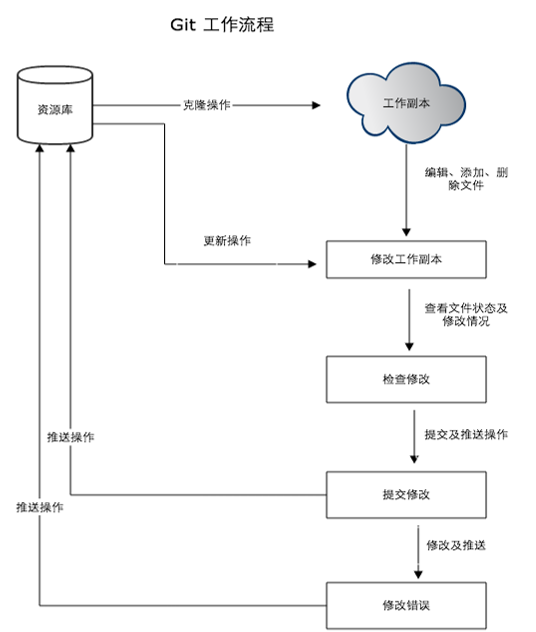
\includegraphics[width=0.7\textwidth]{git.png}
    \caption{git工作流程示意图} % 图片标题
    \label{fig:git} % 图片标签,用于引用
\end{figure}

对自己的仓库进行版本管理主要用到以下这些命令:

\begin{center}
\textbf{git工作流程基本命令}

	\begin{tabular}{c}
		\toprule[1.5pt]
		  git\enspace init       \\
		  git\enspace clone\enspace [url]    \\
		  git\enspace branch\enspace -b\enspace <branch>       \\
		  git\enspace remote\enspace add\enspace origin\enspace [url]       \\
		  git\enspace add       \\
		  git\enspace status       \\
		  git\enspace commit\enspace -m\enspace "description"       \\
		  git\enspace push\enspace <remote>\enspace <branch>:<remote>       \\
		  git\enspace pull\enspace [remote]\enspace [branch]       \\
		\bottomrule[1.5pt]
	\end{tabular}
\end{center}

使用git时我们可以选择直接在终端中通过命令行的方式提交代码,这种方式有时不够直观,因此除了命令行我们还可以使用一些git的图形化工具,比如GitKraken等等,当然也可以直接在clion或vscode中使用git相关插件,这些插件也提供了直观的版本库界面来辅助我们管理代码。



\subsection{conda的简单使用*}

\subsubsection{conda简介}

conda是一个包,依赖和环境管理工具,可以用于在同一个机器上安装不同Python版本的软件包及其依赖,并能够在不同的Python环境之间切换。一个conda环境就是一个目录包含所有的安装包和依赖,不同环境之间独立且不相互影响,跟python的虚拟环境virtualenv一样。通过conda的创建的虚拟环境,我们可以管理不同的python版本及其安装包而无需担心因不同版本导致的冲突;同时,在配置一个新环境时我们还可以利用虚拟环境来试错而不用担心对电脑原生环境造成无法挽回的伤害。

conda适用于多种语言,如: Python,R,Scala, Java,Javascript, C/ C++, FORTRAN等。conda默认随miniconda或anaconda发行。

安装anacoda后,在用户HOME目录下,会有一个anaconda目录,其中bin,include,lib,share里面是conda默认环境的文件,envs存放conda管理的环境信息,pkgs里面是解压的软件安装包。

\subsubsection{conda配置}

conda默认的配置文件为\texttildelow /.condarc,通过修改配置文件我们可以配置如下内容:

\begin{enumerate}
\item conda从哪里获取安装包

\item conda是否使用代理服务器

\item conda从哪里获取环境信息

\item 当conda环境激活的时候是否更新bash提示
\end{enumerate}

\textbf{查看所有配置信息}

\begin{tcode}
	conda config --show --json
\end{tcode}

\textbf{配置使用清华的源}

\begin{tcode}
	conda config --add channels https://mirrors.tuna.tsinghua.edu.cn/anaconda/pkgs/free
	conda config --add channels https://mirrors.tuna.tsinghua.edu.cn/anaconda/pkgs/main
	conda config --set show_channel_urls yes
\end{tcode}

\textbf{配置安装软件时不要提示输入yes}

\begin{tcode}
	conda config --set always_yes true
\end{tcode}

\textbf{取消每次启动自动激活conda的基础环境}

\begin{tcode}
	conda config --set auto_activate_base false
\end{tcode}

建议安装后关闭自动激活,conda环境会和ros2冲突导致ros2的包无法正常编译!!!

\subsubsection{conda基础操作}

这里介绍一些conda命令行的基础操作:

\begin{center}
\textbf{conda基础操作}
	\begin{tabular}{cc}
		\toprule[1.5pt]
		命令 & 作用\\
		\midrule[1pt]
		$  conda\enspace --version    $		&查看当前版本\\
		$  conda\enspace activate\enspace [env]    $		&激活环境\\
		$  conda\enspace deactivate   $		&退出环境\\
		$  conda\enspace update\enspace conda   $		&更新conda\\
		$  conda\enspace create\enspace --name\enspace [env]\enspace python=3.9\enspace [packages...]   $		&创建python 3.9的环境并安装包\\
		$  conda\enspace info\enspace --envs   $		&查看所有的环境\\
		$  conda\enspace list   $		&查看当前环境下的包\\
		$  conda\enspace install\enspace --name\enspace [env]\enspace [package]   $		&安装包到指定环境中\\
		$  conda\enspace remove\enspace --name\enspace [env]\enspace [package]   $		&删除指定环境里的包\\
		\bottomrule[1.5pt]
	\end{tabular}
\end{center}

至此linux部分教程全部结束,相信经过一段时间的熟悉你也能像用windows一样熟练操作linux。当然以上只是linux系统全部功能的冰山一角,更多的操作还望读者在今后的实际工作中自己学习发现,接下来我们将在linux系统上正式开始视觉相关工作的学习。



\section{现代C++技术}
\subsection{走进面向对象编程:类}

\subsubsection{类的基本概念}

类是\textbf{面向对象}(OB,Object-Oriented)最基本的概念,也是C++区别于C语言的重要特征。
面向对象编程的基本思想是抽象出对象,将对象作为程序的基本单元,通过消息传递来进行通信和协作。
对象是类的实例,具有状态和行为,状态存储在对象的数据成员中,行为由对象的方法实现。
对象通过消息传递进行通信,对象之间可以互相发送消息,并处理消息。
面向对象编程的优点是代码的可重用性、可扩展性和可维护性都得到了提高。

在C++中,类是一种抽象数据类型,它定义了对象的行为和状态,并提供了对这些数据的访问接口。
类可以包含数据成员、成员函数、构造函数、析构函数等,这些成员构成了类的接口。
类可以派生出新的类,从而实现代码的重用和扩展。

\begin{tcode}
class ClassName{        //类名
    public:             //修饰限定符public
        ClassName();    //构造函数
        ~ClassName();   //析构函数
        void memberFunction();  //成员函数
    private:                    //修饰限定符private
        int dataMember;         //数据成员
        void privateFunction(); //私有成员函数
}    

\end{tcode}

\begin{enumerate}
    \item \textbf{构造函数和析构函数}:类的构造和析构过程,它们负责对象的初始化和释放,其特点是其函数名与类名相同,没有返回值。
    \item \textbf{成员函数}:实现类的行为,它们实现了类的功能。
    \item \textbf{数据成员}:存储类的数据信息。
\end{enumerate}
\begin{center}

    \begin{tabular}{cc}
        \hline
        修饰限定符 & 作用 \\
        \hline
        private & 只能被类的成员函数使用或调用 \\
        public & 可以被类外的其他函数或派生类中函数调用 \\
        protected & 只能被类的成员函数和派生类使用或调用 \\ 
        \hline
        
    \end{tabular}
\end{center}

% 类可以派生出新的类,派生类可以继承基类的所有成员,并可以添加新的成员。
% 派生类可以重写基类中的成员函数,从而实现新的功能。
% 派生类可以重载基类中的运算符,从而实现新的运算。

面向对象编程的实现方式有多种,包括面向过程、基于消息的、基于事件的、面向对象设计模式等。
面向过程的实现方式是将数据和函数分离,通过函数调用来实现对象之间的通信。
基于消息的实现方式是通过消息传递来实现对象之间的通信,消息可以是函数调用、事件、数据等。
基于事件的实现方式是通过事件驱动模型来实现对象之间的通信,事件可以是用户操作、时间事件、状态变化等。

\subsubsection{静态和友元}

静态成员是指在类外部定义的变量和函数,它属于整个类,而不是类的对象。
静态成员可以\textbf{被类的所有对象}共享,因此可以实现一些全局变量的功能。
静态成员的声明和定义都在类的外部,因此在类的声明中不需要加$static$关键字。

需要特别注意的是,静态变量的定义必须在实例化之前。静态成员的生命周期和整个程序的生命周期是相同的,因此静态成员的构造函数和析构函数只会被调用一次。
\begin{enumerate}
    \item 友元函数:友元函数可以访问类的私有成员,但不能调用类的私有成员函数。
    \item 静态成员:静态成员可以被类的所有对象共享,因此可以实现一些全局变量的功能。
    \item 静态变量:静态变量的定义必须在实例化之前。静态成员的生命周期和整个程序的生命周期是相同的,因此静态成员的构造函数和析构函数只会被调用一次。
\end{enumerate}

\begin{tcode}
class ClassName {
    public:
        ClassName() = default;
    
        ~ClassName() = default;
    
        static void memberFunction();   //成员函数
        static int dataMember;          //数据成员
        friend void FriendFunction(int a, int b);//友元函数定义
    private:                            //修饰限定符private
        static void privateFunction();  //私有成员函数
};
        
void FriendFunction(int a, int b){ //友元函数实现时,不可以添加类的作用域
    std::cout << "你调用了友元函数";
}
        
int ClassName::dataMember = 10; //静态变量只能在类的实例化之前定义
        
int main(int argc, char *argv[]) {
    ClassName obj1, obj2;
    cout << obj1.dataMember << endl;
    cout << obj2.dataMember;
        
    return 0;
}

\end{tcode}

有时,我们希望某个函数可以访问类的私有成员,但又不希望它成为类的成员函数。
这时,我们可以将函数声明为友元函数,并在类的声明中加上$friend$关键字。
友元函数可以访问类的私有成员,但不能调用类的私有成员函数。

\textbf{需要注意的是,不属于类,它破坏了类的封装性,因此不建议使用!}

\subsubsection{函数重载}
\textbf{函数重载(overload)}是指在同一个作用域中,存在多个同名函数,但它们的参数个数或参数类型不同。
函数重载的作用是为了使程序更加灵活,提高代码的可读性和可维护性。

在C++中,函数重载的规则是:
\begin{enumerate}
    \item 函数名相同;
    \item 参数个数不同;
    \item 参数类型不同。
\end{enumerate}

\begin{tcode}
class ClassName {
public:
    ClassName() = default;

    ~ClassName() = default;

    int CalSum(int a,int b){
        return a+b;
    }

    double CalSum(double a,double b){
        return a+b;
    }
};

int main(int argc, char *argv[]) {
    ClassName obj;
    cout << obj.CalSum(1,2) << endl;
    cout <<  obj.CalSum(1.5,2.5);

    return 0;
}
\end{tcode}

在上例中,CalSum函数的两个版本都可以接受两个参数,但它们的返回值和参数类型不同。
因此,我们可以实现两个函数的重载,使得程序更加灵活。在执行函数时,编译器会根据函数的调用情况,自动选择最匹配的函数版本。

\textbf{构造函数的类型:}

\begin{enumerate}
    \item 默认构造:默认构造函数是指没有参数的构造函数,它会创建一个对象,并对其进行初始化。
    \item 含参构造:含参构造函数是指有参数的构造函数,可以根据参数的值对对象进行初始化。
    \item 拷贝构造:拷贝构造函数是指将一个对象拷贝到另一个对象时,会调用拷贝构造函数。
\end{enumerate}

\begin{tcode}
#include<iostream>
#include<string>
class ClassName {
public:
    ClassName():member(1) //初始化列表
    {std::cout << "你调用了默认构造函数" << std::endl;}
    ClassName(std::string& str) 
    {std::cout << "你调用了含参构造函数,参数是" << str << std::endl;member=2;}
    ClassName(ClassName &obj) //这里必须是引用传参,思考一下为什么
    {std::cout << "你调用了拷贝构造函数" << std::endl;
    this->member = obj.member;}
    ~ClassName() = default;

    int member;
};

int main(int argc, char *argv[]) {
    ClassName obj1;
    std::string str = "Hello World";
    ClassName obj2(str);
    obj1.member = 10;
    ClassName obj3(obj1);

    std::cout << "obj1:" << obj1.member << std::endl;
    std::cout << "obj2:" << obj2.member << std::endl;
    std::cout << "obj3:" << obj3.member << std::endl;

    return 0;
}
\end{tcode}
有一些tips可以快速设置构造函数
\begin{tcode}
ClassName() = default;              //默认构造函数,使用默认的方式
ClassName(ClassName& obj) = delete; //禁止拷贝构造,单例实现对象
\end{tcode}
\textbf{运算符重载:}

在C++中,类提供了一个接口,可以将运算符进行重载,从而实现对类更加灵活的操作。
运算符重载的语法如下:

\begin{tcode}
[返回值] operator [操作符] ([参数列表]) {
    //操作符的实现
}
\end{tcode}

示例:

\begin{tcode}
class ClassName {
    public:
        ClassName():a(1),b(2) {}
    
        ClassName& operator+(ClassName& obj){//重载加法运算符
            this->b += obj.b;   //this指针,指向自己
            this->a += obj.a;
            std::cout << "这里执行过了" << std::endl;
            return *this;   //*this表示当前对象的引用
        }
     
        //重载流插入运算符,思考一下为什么是这样写?
        friend std::ostream& operator<<(std::ostream& out, ClassName& obj);
    
        int a;
        int b;
    };
    
    std::ostream& operator<<(std::ostream& out, ClassName& obj){
        out << "a:" << obj.a << " b:" << obj.b << std::endl;
        return out;
    }
    
    int main(int argc, char *argv[]) {
        ClassName obj1;
        ClassName res = obj1 + obj1;
        std::cout << res;
    
        return 0;
    }
\end{tcode}

\textbf{$this$指针}是一个隐指针,指向这个类本身。
在类的成员函数中,$this$指针可以用来访问类的成员变量和成员函数。
在类的构造函数中,$this$指针可以用来初始化类的成员变量。
一般情况下,$this$指针可以不写,编译器会自动生成。但是有些情况,处于项目代码可读性的目的,会写显性的$this$指针。
此外,类中成员函数的第一个参数必须是$this$指针,表示当前对象的引用。这也是类的成员函数的调用方式。在后面我们会详细解释类的执行方式,此处略去不表。

\subsubsection{类的继承}
类的继承是面向对象编程的重要特征之一,它允许创建新的类,从而继承基类的成员,并添加新的成员。

\begin{figure}[H]
    \centering
    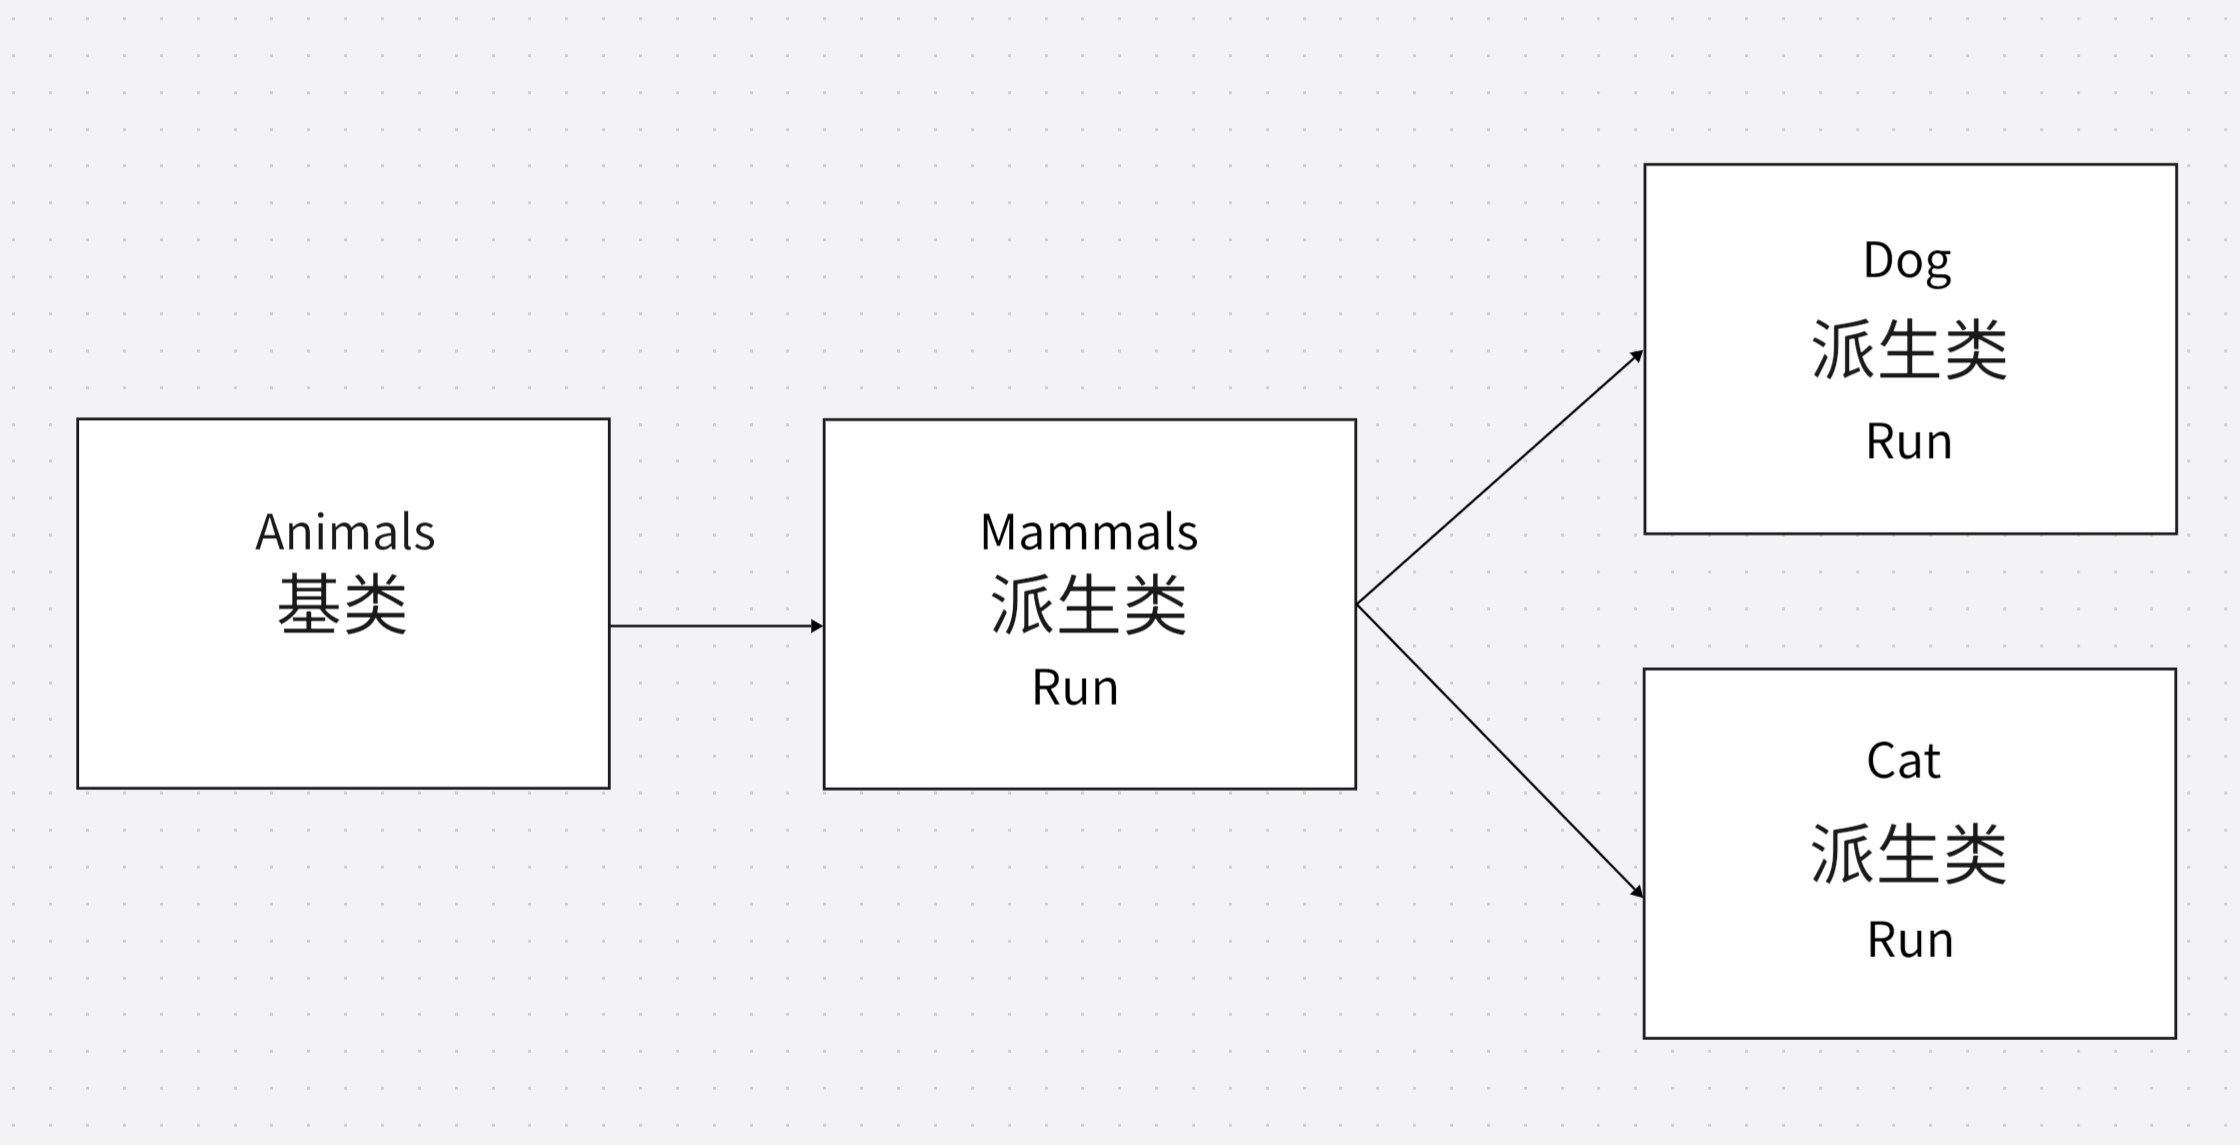
\includegraphics[width=0.7\textwidth]{A111.png}
    \caption{类的继承} % 图片标题
    \label{fig:A111} % 图片标签,用于引用
\end{figure}

如图\ref{fig:A111}所示,派生类从基类中继承了数据成员和成员函数,并可以添加新的成员。
派生类可以重写基类中的成员虚函数,从而实现新的功能。
派生类可以重载基类中的运算符,从而实现新的运算。

\begin{center}
\textbf{继承的三种方式:}

    \begin{tabular}{cccc}
        \hline
        访问 & public & private & protected \\
        \hline
        同一个类 & yes & yes & yes \\
        派生类 & yes & no & yes \\
        类外部 & yes & no & no \\ 
        \hline
        
    \end{tabular}
\end{center}

继承可以用下面的写法实现:

\begin{tcode}
class Shape {//这个基类只含有纯虚函数,又叫做抽象类
public:
    Shape() = delete;
    Shape(double A):Area(A)
    {std::cout << "基类的构造函数已经被调用" << std::endl;}
    virtual double calArea() = 0; //这里是纯虚函数,也可以使用普通函数
    double Area;
};

class Rectangle
        : protected Shape{
public:
    Rectangle() = delete;
    Rectangle(double a,double b):a(a),b(b),Shape(a*b)
    {std::cout << "Rectangle类的构造函数已经被调用,面积为" << Area << std::endl;}
    double a;
    double b;
    double calArea() override{  //重写基类的函数
        return a*b;
    }

};

class Circle
        :Shape{
public:
    Circle() = delete;
    explicit Circle(double r):r(r),Shape(3.14*r*r)
    {std::cout << "Circle类的构造函数已经被调用,面积:" << Area << std::endl;}
    double r;
    double calArea() override{
        return 3.14*r*r;
    }

};

int main(int argc, char *argv[]) {
    Circle circle(1.0);
    Rectangle rect(1.0,2.0);
    return 0;
}
\end{tcode}


 \subsubsection{模版}
在开发过程中,我们可能会遇到这样的场景,我们有一个函数或者类,但是它只适用于特定的数据类型,
比如$int$或者$double$。为了实现对这两种类型都可以调用函数,
就会遇到需要复制一遍代码,但是这样做就造成了代码冗余,不利于维护。这时候就需要用到模版($template$)。

模版是C++中一个重要的特性,它允许我们定义一个类或函数,使其可以接受不同的数据类型或者不同的参数。
模版的定义和使用都比较复杂,这里只介绍最基本的用法。
使用$class$关键字声明类型,使用具体的类型声明参数
\textbf{函数模版}的语法如下:
\begin{tcode}
template<class T>
T function(T a){
    return a;
}

auto funcPtr = function<int>;
template<int A>
int function(){
 return A;
}

auto funcPtr = function<2>;
template<class T,T A>
T function(){
 return A;
}
auto funcPtr = function<int,2>;
\end{tcode}

 这里的$class \quad T$表示一种数据类型,可以是任意类型。
 在函数的定义中,$T$可以作为函数的参数,也可以作为函数的局部变量。在使用函数模板时,需要首先进行函数的实例化。

\begin{tcode}
//调用的时候实际上分为两步,实例化和调用
function<int>(10);
function<double>(20.0);
//在编译器可以推导出类型的时候可以不加<>
auto a = function(1.0);
//在无法推导的时候,要先进行实例化
std::function<int(int)> ptr = function<int>;
\end{tcode}

模版的优点:
\begin{enumerate}
    \item 代码重用性高:可以定义一个通用的函数,然后根据需要实例化不同的类型,实现代码的重用。
    \item 类型安全:模版可以保证类型安全,避免类型错误。
    \item 效率高:模版可以提高效率,因为编译器可以对代码进行优化。
\end{enumerate}

\textbf{类模版}:
类模板的语法和函数模板类似,只不过在类名而不是函数名前面加上关键字$template$。
在普通类中也可以添加成员函数模版,只需要在函数名前面加上关键字$template$即可。

\begin{tcode}
template<class T1,class T2>
class A{
    A() = default;
    ~A() =default;
    T1 val;
    T2 id;
    T1 function(T1* a, T2& b){
        return *a+b++;
    }
};
\end{tcode}

在$template$后面,可以定义多个类型参数,用逗号分隔。需要注意的是,在类中的函数模版需要再头文件中实现,
也就是说,模版的声明和实现不可以分离,否则会出现很多问题。
对于类模板也可以实现继承和多态,与普通类相同,这里不在展开,感兴趣的同学可以自行探索。

\textbf{模板的实例化}:
模板的实例化指的是将模板定义和具体的类型绑定在一起,生成一个具体的类或函数。
在类的实例化时,$<>$的内部需要填写一个可以推导出的数据类型,编译器会根据类型推导出模板的具体类型。
一般来说,实例化有以下几种方式:

\begin{enumerate}
    \item 具体类型:如$int$,$double$等基本类型,$struct$,$class$,$union$等复合数据类型,$int*$,$double\&$等指针和引用类型
    \item 编译期可以确定的常数:字面常量,宏,$constexpr$
    \item 显示实例化:在编译时,通过命令行指定具体的类型
\end{enumerate}

除此之外,还有一种变参模版,它可以接受任意数量的类型参数,但是在实例化时,必须指定具体的类型。
这种情况比较复杂,这里不在展开。感兴趣的同学自行探讨:

\url{https://blog.csdn.net/fl2011sx/article/details/128077440}


\subsection{魔法代码:C++17}


随着时代的发展和项目变得越来越复杂,人们创造了一系列新的代码特性,其中一些特性在C++11和C++17中被引入,
在不熟悉这些特性的人看来,这些代码看上去显得十分无厘头,甚至有些难以理解。本章将介绍C++11和C++17中引入的一些新的代码特性,
并通过实例来说明它们的用法。
\subsubsection{lambda表达式}

\textbf{指名初始化(Designated Initializers)}是一种初始化聚合类型(Aggregate Types)成员的方式,
这种方式允许你指定每个成员的初始化值,而不必按照成员在聚合类型中的声明顺序进行初始化。
这种方式在C++11标准中被引入。他的语法很简单:

\begin{tcode}
//类型名 对象名{成员名1 = 初始值1, 成员名2 = 初始值2,...};
struct Foo {int a, b};
Foo foo = {.b = 3, .a = 1};
\end{tcode}

\textbf{匿名函数(anonymous function)}是一种在程序中定义的函数,它没有名字,只能在运行时创建。C++11引入了lambda表达式,
它是一种更简洁的语法,可以用来创建匿名函数。lambda表达式的语法如下:

\begin{tcode}
完成版:[捕获列表](参数列表) mutable throw(异常列表) -> 返回值 {函数体}
简化版:[捕获列表](参数列表) {函数体}
\end{tcode}    

\begin{enumerate}
    \item 捕获列表:捕获列表可以用来捕获外部作用域中的变量,使得lambda表达式可以访问这些变量。捕获列表的语法如下:
    \item 参数列表:参数列表定义了lambda表达式的参数,可以有0到多个参数。
    \item mutable[可选]:mutable关键字用来声明lambda表达式的捕获列表中的变量是可修改的。
    \item throw(异常列表)[可选]:throw关键字用来指定lambda表达式可能抛出的异常。
    \item 返回值:返回值定义了lambda表达式的返回类型。
    \item 函数体:函数体定义了lambda表达式的主体,可以是一条表达式或多条语句。
\end{enumerate}

\begin{tcode}
#include<iostream>
#include<functional>

template<class T>
void sort(T* array,int n,std::function<bool(T&,T&)> compare){
    for(int i=0;i<n;i++){
        for(int j=i;j<n;j++){
            if(!compare(array[i],array[j])){    //为false时,交换(按照指标降序)
                std::swap(array[i],array[j]);
            }
        }
    }
}

typedef struct Block{
    char ch;
    int id;
}Block;

int main(int argc, char *argv[]) {
    auto sum = [](int a,int b){
        return a+b;
    };

    std::cout << sum(1,2) << std::endl;

    Block blocks[5]={{'a',2},{'d',4},{'q',1},{'t',7},{'s',-1}};
    sort<Block>(blocks,5,[](Block& a1,Block a2){//lambda表达式作为参数传递
        return a1.id > a2.id;
    });
    for(int i=0;i<5;i++){
        std::cout << "ch:" << blocks[i].ch << "  id:" << blocks[i].id << std::endl;
    }
    return 0;
}
\end{tcode}    

\textbf{捕获列表:}可以捕获外部作用域中的变量,包括this指针。捕获的方式包括两种,即值捕获和引用捕获。


\begin{center}

    \begin{tabular}{ccccc}
        \hline
        捕获方式 & 拷贝方式 & 是否可以修改值 & 语法 & 全捕获\\
        \hline
        值捕获 & 通常深拷贝  & 否 & [a,b] & [=]\\
        引用捕获 & 浅拷贝 & 是 & [\&a,\&b] & [\&]\\
        \hline
        
    \end{tabular}
\end{center}

如果使用值捕获,这里是否是深拷贝取决于拷贝构造函数,如果拷贝构造函数中是移动或者引用语义,
那么遵从拷贝构造的语义。
但是这个值会被设置成不可操作的状态,他的值被视为常量,不能被修改。
这时,可以使用mutable关键字来声明这个值是\textbf{可修改}的。

\begin{tcode}
int a = 0;
auto f = [a]() mutable {
    return ++a;//如果不写mutable,编译器会报错
};
\end{tcode}

使用lambda表达式可以简化代码,提高可读性。由于捕获列表的存在,使得lambda表达式可以访问外部作用域的变量,
相比于普通函数,lambda表达式更加灵活。
lambda表达式的返回值是一个函数指针,可以作为函数参数进行传递。也可以使用function承接返回值。
\begin{tcode}
//使用function承接返回值
std::function<int(int,int)> add = [](int a,int b){return a+b;};
int result = add(1,2);//调用lambda表达式
//也可以使用auto关键字自动推导返回类型
auto sub = [](int a,int b){return a-b;};
\end{tcode}

在C++14和C++17中,lambda表达式增加了一些新的用法,使用这些新的特性可以简化代码,更加灵活地解决实际问题。

\textbf{泛型Lambda表达式:} 
可以使用auto关键指定形参的类型,从而快速地实现函数\textbf{泛用}。这也是\textbf{泛化编程}的一种方式,感兴趣的同学可以自行了解。
\begin{tcode}
auto f=[](auto a,auto b){return a+b;};
std::cout << f(1,2) << " " << f('a',2.0) << std::endl;
\end{tcode}

\textbf{this指针捕获:} 
可以使用[this]的方式捕获类中的$this$指针,$this$和$*this$都可以。
给一个简单的例子,可以自己理解:
\begin{tcode}
class A{
private:
    int a;
public:
    A(){
        auto function = [this](){//[]中使用*this作用相同
            return a+1;
        };
    }
};
\end{tcode}

\textbf{初始化捕获:}在C++17中,可以使用初始化捕获来简化代码。
可以初始化一个变量,并将其绑定到lambda表达式中,这样就不需要再使用声明这个变量了。

\begin{tcode}
auto f = [a=1]() mutable {
    return a;
};
\end{tcode}

\subsubsection{引用和移动}
\textbf{左值与右值:}
左值一般为我们自己定义的变量,在定义时开辟了内存,我们可以对这块内存赋值,修改内存中的值,如果有const也仅从语法层面上不允许修改,这块内存在其生命周期结束的时候销毁。

右值一般为临时变量,是程序运行时产生的中间产物,他不是我们用户自己定义开辟空间的,是由编译器帮我们开辟空间,并且在用完就立即销毁。右值的生命周期一般只在当前语句,当我们要对右值进行赋值时,他已经释放空间了,此时我们再进行访问就是野访问,(与野指针一样造成内存问题),所以我们不能对右值进行修改,编译器强制语法检查,遇到修改操作就报错。

右值中特殊的就是字面常量,他们存储在内存的常量区,内存为只读属性,不可以修改,不可以取地址,他们的生命周期与程序的生命周期一样,当我们使用字面常量时,编译器帮我们开辟空间,并用字面常量初始化,这块临时空间用完即销。
\textbf{分辨左右值最常用方法就是判断他是否可以取地址。如果不可以就为右值。}
\begin{tcode}
int a;
a = 10;//这个赋值过程中,a是左值,b是右值(字面常量)
int b;
b = a;//这个赋值过程中,a是右值,b是左值
//10 = a;//这样的语句显然是错误的,即右值不能被修改
\end{tcode}
显而易见的是,左值可以被隐式地转换为右值,而右值不可以被转换为左值(从这一点上看,右值类似于常量)。

\textbf{引用:}
C++的引用是一种别名,用于引用已存在的变量。引用一旦初始化,就不能再引用其他变量。在创建引用时,编译器不会重新开辟内存,而是直接引用已存在的内存(这一点引用类似于指针)。
引用的主要用途包括函数参数传递和返回值优化。使用引用可以避免复制,提高效率,特别是在处理大型对象时。
引用通过 \& 符号来声明。例如:
\begin{tcode}
int& ref = var;
\end{tcode}
这段代码创建了一个名为 $ref$ 的引用,它引用了变量 $var$。引用分为两种,左值引用(\&)和右值引用(\&\&)。
顾名思义,左值引用只能绑定一个左值,而右值引用只能绑定一个右值。

首先说左值引用,这个十分简单,可以认为是去别名,操作左引用就相当于操作被绑定的那个左值本身,这一点就算在函数传参过程中也是如此。
\begin{tcode}
void func(int& A){//可以试一下把引用去掉
    A *= 2;
}

int main(int argc, char *argv[]) {
    int a = 10;
    func(a);
    return 0;
}
\end{tcode}
在这里a的值被修改为20,因为传入$func()$的a是引用,所以操作的是a本身,而不是a的拷贝。
这就是引用在传参和提高函数效率上的用处。

再说右值引用,这个就有点复杂了,右值引用是为了解决左值引用不能绑定右值的限制。
\begin{tcode}
void func(int&& a){
    std::cout << "a的地址:" << &a << std::endl;
    a *= 2;
}

int main(int argc, char *argv[]) {
    int&& c = 10;
    std::cout << "c的值为:" << c << std::endl;
    func(c);
    std::cout << "经过函数之后,c的值为:" << c << std::endl;
    std::cout << "c的地址为" << &c << std::endl;
    return 0;
}
\end{tcode}

哎?这就很奇怪,为什么c的值被修改了?为什么c的地址可以取到?为什么作为右值的c的值被修改了?这说明右值引用绝对不是简单的取别名,他的作用更加复杂。

根据我们上面的解释,编译器在执行完第6行的代码之后,自动帮我们析构了10这个右值。
但是实际情况是,由于我们使用了右值引用,\textbf{对内存空间的操控权转交给了我们,没有进行自动析构}。

话又说回来,为什么a的地址和c是相同,这完全就是左值引用的用法啊?是的,在C++中,\textbf{右值引用会被自动地当做为左值来使用}。
而在函数传参时,两种引用就没有什么分别了。

看到这里,我们不禁想要问这样的一个问题了,既然右值引用可以被自动转换为左值来使用,为什么还要使用右值引用呢?
C++的设计师是闲的吗,每天整这么多概念来为难我们?当然不是!还记得我们刚才说的,左值引用是不能绑定右值的,
那如果我们想要使用右值,那岂不是每次都要拷贝一份了吗?这显然是不合理的。设想一下,如果有一个超级大的对象,我们每次都只能拷贝一份,那效率岂不是太低了?
所以,C++的设计者们想到了一个折中的办法,既能避免拷贝,又能保证效率,就是使用右值引用。
\begin{tcode}
#include <iostream>
class A {
public:
    A() : val("a0") { std::cout << "你调用了默认构造" << std::endl; }

    A(std::string a) : val(a) { std::cout << "你调用了含参构造" << std::endl; }

    A(A &obj) {
        std::cout << "你调用了拷贝构造" << std::endl;
        this->val = obj.val;
    }

    A(A &&obj) noexcept {
        std::cout << "你调用了移动构造" << std::endl;
        this->val = std::move(obj.val);
    }

    A &operator=(A &obj) {
        if (this == &obj)
            return *this;
        std::cout << "你调用了等号赋值" << std::endl;
        this->val = obj.val;

        return *this;
    }

    ~A() { std::cout << "对象被析构,val为:" << val << std::endl; }

    std::string val;
};

int main(int argc, char *argv[]) {
    std::cout << "a1,";
    A a1("a1");
    std::cout << std::endl;

    std::cout << "a2,";
    A a2 = a1;
    std::cout << "val值为:" << a2.val << std::endl;
    std::cout << std::endl;

    a2 = a1;//区别上面的
    std::cout << std::endl;

    std::cout << "a3,";
    A a3(a2);
    std::cout << "val值为:" << a3.val << std::endl;
    std::cout << std::endl;

    std::cout << "a4,";
    A &a4 = a1;
    std::cout << "val值为:" << a4.val << std::endl;
    std::cout << std::endl;

    std::cout << "a5,";
    A &&a5 = std::move(a1);
    std::cout << "val值为:" << a5.val << std::endl;
    std::cout << std::endl;

    a2.val = "new a2";
    std::cout << "a1的val值为:" << a1.val << std::endl;
    a4.val = "new a4";
    std::cout << "a1的val值为:" << a1.val << std::endl;
    std::cout << "a5的val值为:" << a5.val << std::endl;
    std::cout << std::endl;

    std::cout << "a6,";
    A a6(std::move(a1));
    std::cout << "val值为:" << a6.val << std::endl;
    std::cout << "a1被传入移动构造后,";
    std::cout << "val值为:" << a1.val << std::endl;
    std::cout << std::endl;


    return 0;
}
\end{tcode}
请读者,仔细体会一下这段代码的输出。

\textbf{移动语义:}
首先了解一个std中函数move,他的作用是将参数类型强制转换为右值,不管参数是左值还是右值。
\begin{tcode}
using namespace std;
void Fun(int& x) { cout << "左值引用" << endl; }
void Fun(const int& x) { cout << "const 左值引用" << endl; }
void Fun(int&& x) { cout << "右值引用" << endl; }
void Fun(const int&& x) { cout << "const 右值引用" << endl; }

int main() {
    PerfectForward(10);           // 右值
    int a = 1;
    Fun(a);            // 左值
    Fun(std::move(a)); // 右值
    const int b = 8;
    Fun(b);      // const 左值
    Fun(std::move(b)); // const 右值
    return 0;
}
\end{tcode}
如代码所见,当我们使用std::move()时,编译器将左值引用转换为右值引用。

再介绍一种利用模版实现完美转发的方式。在模板中,T\&\&可以接收左值和右值,要利用到forward<>()函数,他会保留引用的类型,并将其转发给另一个函数,
否则,传参的引用都会被转换为左值引用。

\begin{tcode}
using namespace std;
void Fun(int& x) { cout << "左值引用" << endl; }
void Fun(const int& x) { cout << "const 左值引用" << endl; }
void Fun(int&& x) { cout << "右值引用" << endl; }
void Fun(const int&& x) { cout << "const 右值引用" << endl; }

template<typename T>
void PerfectForward(T&& t)
{
    Fun(t);
    //Fun(std::forward<T>(t));//使用完美转发
}

int main() {
    PerfectForward(10);           // 右值
    int a = 1;
    Fun(a);            // 左值
    Fun(std::move(a)); // 右值
    const int b = 8;
    Fun(b);      // const 左值
    Fun(std::move(b)); // const 右值
    return 0;
}
\end{tcode}
左引用和右引用的概念比较容易混淆,要在实践中不断运用,才能熟练掌握。

\subsubsection{智能指针}
对于有些使用场景,比如动态申请数组,我们会用到$new$和$delete$操作符(等价于C语言中的malloc和free操作符),
但是当我们忘记释放内存时,就会出现\textbf{内存泄漏}的问题。但是随着项目越来越大,函数嵌套越来越深,
对于变量的生命周期管理也变得十分复杂,我们总不能每次都想着释放内存吧?这样做也太繁琐了,那么怎么解决这个问题呢?

C++11引入了智能指针,它是一种用来管理动态内存的技术。智能指针的主要作用是自动地管理堆内存的分配和释放,
从而避免内存泄漏和内存泄露。智能指针的主要类型有\textbf{$shared\_ptr$}、\textbf{$unique\_ptr$}和\textbf{$weak\_ptr$}。

智能指针是一个类,当这个类被析构的时候,他会自动释放其管理的内存。
根据使用场景的不同,可以选择使用不同的智能指针。
我们来一个一个看:

\begin{tcode}
//class A和class B的定义
class A;
class B;
class A{
public:
    A(){std::cout << "你调用了A的默认构造函数" << std::endl;}
    ~A(){std::cout << "A对象已被析构,val值为:" << val << std::endl;}
    int getVal(){return val;};
    void setVal(int val){this->val = val;}
    std::shared_ptr<B> B_ptr;
private:
    int val;
};

class B{
public:
    B(){std::cout << "你调用了B的默认构造函数" << std::endl;}
    ~B(){std::cout << "B对象已被析构,val值为:" << val << std::endl;}
    int getVal(){return val;};
    void setVal(int val){this->val = val;}
    std::shared_ptr<A> A_ptr;
private:
    int val;    
};
\end{tcode}

\textbf{unique\_ptr:} 
$unique\_ptr$是一种独占式智能指针,它只能拥有一个指向的资源,一旦资源被释放,它就不能再被使用。
当$unique\_ptr$指向一个资源时,它会自动管理资源的生命周期,当$unique\_ptr$离开作用域时,它会自动释放资源。

\begin{tcode}
{
    std::unique_ptr<A> ptr1 = std::make_unique<A>();
    ptr1->setVal(1);
    //std::unique_ptr<A> ptr2 = ptr;会报错
    std::unique_ptr<A> ptr2 = std::move(ptr1);
    if(ptr1 == nullptr){
        std::cout << "ptr1是一个空指针" << std::endl;
    }
    std::cout << "ptr2的val值为:" << ptr2->getVal() << std::endl;
    ptr1 = std::make_unique<A>();
    ptr1->setVal(2);
}
\end{tcode}
由于$unique\_ptr$的拷贝构造和赋值运算符被禁用,所以不能通过拷贝构造或赋值来获取资源的副本。因此,
$unique\_ptr$只能被移动,不能被复制。

\textbf{shared\_ptr:}

在实际的使用过程中,我们可能会遇到这样的场景,我们想要让两个指针同时指向同一个资源,
但是由于unique\_ptr的特性,这个操作不可以在其上实现,这时shared\_ptr就排上用场了。
shared\_ptr可以有多个指向的资源,它引用了一个计数机制,记录了当前资源被多少个指针指向。
当资源的引用计数为0时,它会自动释放资源。

\begin{tcode}
{
{
    std::shared_ptr<A> ptr1 = nullptr;
    {
        auto ptr2 = std::make_shared<A>();
        ptr2->setVal(1);
        ptr1 = ptr2;
        //ptr1 = std::move(ptr2);//看一下这两种有什么区别?
        std::cout << "ptr1对象的引用次数为:" << ptr1.use_count() << std::endl;
        std::cout << "ptr2对象的引用次数为:" << ptr2.use_count() << std::endl;
    }
    std::cout << "ptr2已经被析构了" << std::endl;
}
}
\end{tcode}
可以看到,$shared\_ptr$可以进行拷贝和移动操作,$shared\_ptr$在进行移动操作时,会将资源的所有权转移到目标指针上,
指针的计数没有增加,而原来的指针将会丢失其中的内容。拷贝操作则会增加引用计数,原来的指针和目标指针都指向同一个资源。
当其中一个智能指针被析构时,引用计数减1,但对象不会被析构,直到所有指向它的指针都被销毁。当引用计数为0时,资源会被释放。

\textbf{weak\_ptr:}

看一下下面的例子

\begin{tcode}
int main(int argc, char *argv[]) {
{
    std::shared_ptr<A> pA(new A);
    std::shared_ptr<B> pB(new B);

    std::cout << pA.use_count() << std::endl;
    std::cout << pB.use_count() << std::endl;
}
std::cout << "上面是符合我们预期的" << std::endl << std::endl;
{
    std::shared_ptr<A> pA(new A);
    std::shared_ptr<B> pB(new B);

    pA->B_ptr = pB;
    pB->A_ptr = pA;

    std::cout << pA.use_count() << std::endl;
    std::cout << pB.use_count() << std::endl;
}
std::cout << "咦?这是什么情况呢?为什么没有被析构呢?" << std::endl;
return 0;
}
\end{tcode}
原来,pA和pB已经分别指向了A和B,但是当我们将它们互相引用时,
A\_ptr和B\_ptr也指向了A和B,当pA和pB被析构时,A\_ptr和B\_ptr并没有被析构,他们的引用次数变成了1,
因此A和B并不会被析构。如果类A、B里面有从\textbf{堆内存}中申请的资源,那就发生\textbf{内存泄漏}了。这显然是不正确的,所以需要引用$weak\_ptr$。

$weak\_ptr$是一种弱引用指针,它指向一个资源,但是不能操作这个资源,只能以一种“观察者”的身份“观察”资源。
将class A和class B中的A\_ptr和B\_ptr改为weak\_ptr,就可以解决这个问题。

\begin{tcode}
{
    std::shared_ptr<A> pA(new A);
    std::shared_ptr<B> pB(new B);

    pA->B_ptr = pB;
    pB->A_ptr = pA;

    std::cout << pA.use_count() << std::endl;
    std::cout << pB.use_count() << std::endl;
}
\end{tcode}
但是,新的问题出现了:$weak\_ptr$只是对象的观察者,不拥有对象本身。
从实现上看,$weak\_ptr$没有重载 "operator *" 和 "operator ->",自然无法使用资源了。
该如何解决这个问题呢?解决方案就是对资源上锁,将$weak\_ptr$升级为$shared\_ptr$,这样就可以使用资源了。

\begin{tcode}
{
    std::shared_ptr<A> pA(new A);
    std::shared_ptr<B> pB(new B);

    pA->B_ptr = pB;
    pB->A_ptr = pA;

    std::cout << pA.use_count() << std::endl;
    std::cout << pB.use_count() << std::endl;

    std::shared_ptr<A> PtrA = pB->A_ptr.lock();
    if(PtrA!= nullptr)//确保PtrA不为空,线程安全
        PtrA->setVal(1234);
    PtrA.reset();//别忘了reset释放PtrA
}
\end{tcode}
这种抓住资源的动作,其实在\textbf{多线程}的环境中非常有用,在使用共享资源的时候,其实共享资源可能已经被释放了,
但本线程并不知道。而有了lock函数之后,就可以尝试“抓住资源”,如果返回不是nullptr,那就可以正常的使用资源了。
关于多线程的安全问题,会在后面进行讲解。

总结一下三种智能指针:
\begin{center}

    \begin{tabular}{cccc}
        \hline
        智能指针 & 指向数量 & 析构条件 & 是否可操作资源\\
        \hline
        unique\_ptr & 只能一个 & 出存活域 & 是\\
        shared\_ptr & 可以多个智能指针指向同一个 & 指向计数为0 & 是\\
        weak\_ptr & 可以多个智能指针指向同一个 & 指向计数为0 & 否\\
        \hline
        
    \end{tabular}
\end{center}

\subsubsection{初探STL标准容器}
\textbf{数据结构:}
所谓数据结构,就是指数据的组织、存储、操作和处理方式。数据结构是计算机科学中非常重要的概念,
它是指数据的集合、结构、关系和变化的描述。数据结构是计算机科学中最基本的概念之一,
是计算机程序设计的基础。数据结构是指数据的集合、结构、关系和变化的描述。
基本的操作有四:\textbf{插入、删除、改动、查找}(增删改查)。


下面我们将简单介绍几种常见的数据结构,以及他们的STL容器:

\begin{enumerate}
    \item \textbf{数组}:数组是最基本的数据结构,它是一组相同类型的数据,按照顺序存储在一块连续的内存中。
    \item \textbf{链表}:链表是一种非连续的内存块,它是由一系列节点组成,每个节点都包含数据和指针。
    \item \textbf{队列}:队列是一种线性数据结构,它只允许在一端进行插入操作,在另一端进行删除操作。
    \item \textbf{优先队列}:优先队列是一种特殊的队列,它允许插队的出现,可以根据“重要性”对队中元素进行排序。
    \item \textbf{堆栈}:堆栈是一种线性数据结构,它只允许在一端进行插入和删除操作。
    \item \textbf{树}:树是一种无向图,其中不存在环路,且任意两个结点之间有且仅有一条简单路径相连。
    \item \textbf{二叉树}:二叉树是一种特殊的树,要么没有根节点,是一颗空树
    ;要么由根节点、左子树、右子树组成,且左子树和右子树都是二叉树。
    \item \textbf{堆}:堆是一种特殊的树,它是一个完全二叉树,每个节点都有一个值,并且每个节点都大于或等于其子节点。
\end{enumerate}

他们的头文件如下:

\begin{tcode}
#include <array>    //静态数组array
#include <vector>   //动态数组vector
#include <list>     //链表list
#include <queue>    //队列queue 优先队列priority_queue
#include <stack>    //堆栈stack
#include <map>      //映射map 是一种快速查找关联容器
\end{tcode}

需要注意的是,上面所列举的数据结构类型并不是并列的,三大数据结构分别是:线性表(包括1、2、3、4、5)
,树(包括6、7、8),图(太复杂,暂时不介绍)。

\textbf{数组}:数组是最基本的数据结构,它是一组相同类型的数据,按照顺序存储在一块连续的内存中,如图\ref{fig:数组}。

\begin{figure}[H]
    \centering
    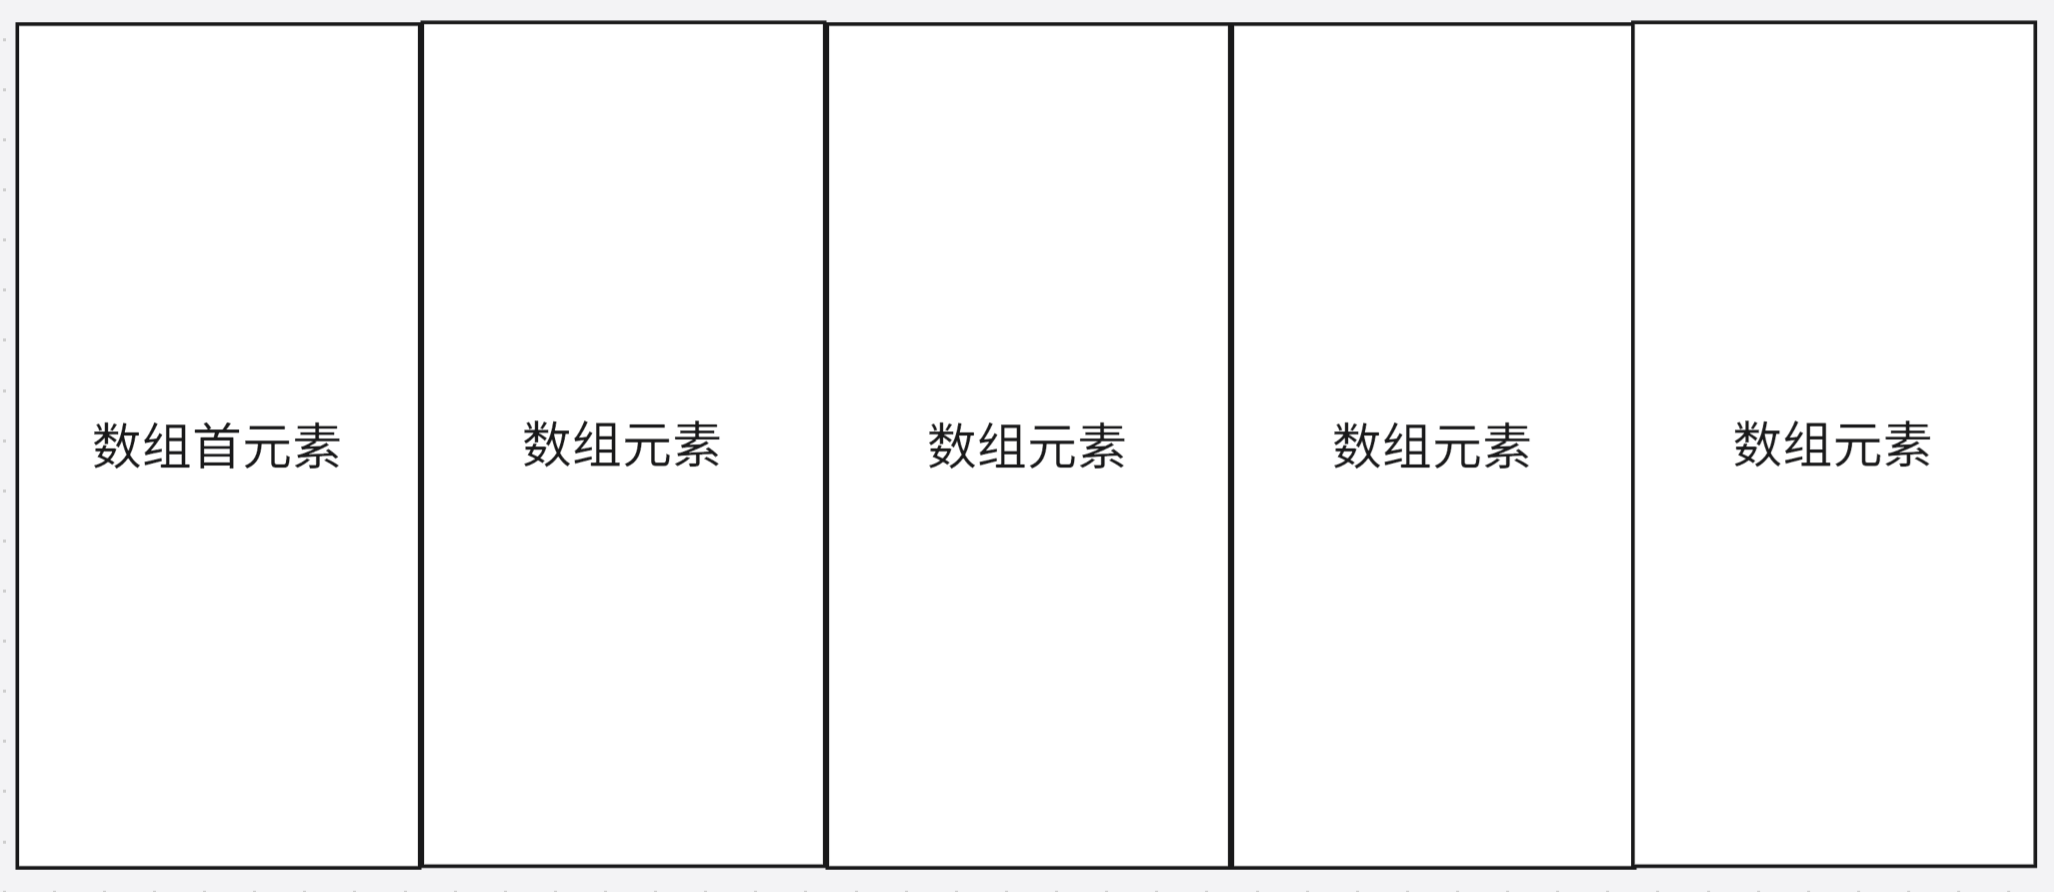
\includegraphics[width=0.7\textwidth]{数组.png}
    \caption{数组} % 图片标题
    \label{fig:数组} % 图片标签,用于引用
\end{figure}

\textbf{数组(Array)},又称\textbf{顺序表},它的STL容器有两种,分别是$array$和$vector$。

$array$是固定大小的数组。$vector$是一种动态数组,可以动态增长,可以根据需要自动分配内存。两者的声明方式如下:
\begin{tcode}
std::array<int,5> arr;
std::vector<int> vec;
\end{tcode}

$array$并不常用,因为它是固定大小的,如果需要改变大小,只能重新声明一个新的数组。
可以参考这篇blog详细了解:

\url{https://blog.csdn.net/qq_38410730/article/details/102802239}

$vector$由于其动态性,可以根据需要自动分配内存,因此使用起来比较方便,在工程实践中也更常用。
$vector$的实现原理是当检测到$vector$的容量不足时,会自动分配新的内存(原来的大小$\times$2),并将原有数据复制到新内存中。
这个复制的过程非常缓慢,因此,在使用大型的资源时,$vector$的效率可能会比较低。

成员函数(常用部分):
\begin{tcode}
std::vector<int> vec{1,2,3,4,5,6};
vec[0];         //访问(快速)
vec.at(0);    //访问(安全)
vec.front();    //第一个元素
vec.back();     //最后一个元素
vec.empty();    //检查是否为空
vec.size();     //返回容器大小
vec.reserve(10);//预留空间
vec.clear();    //清除所有元素
vec.insert(vec.begin(),1);//插入元素
vec.erase(vec.begin());//删除元素
vec.push_back(1); //在最后添加
vec.emplace_back(); //在最后添加
vec.pop_back();     //删除最后一个
\end{tcode}

\textbf{链表(List)}:链表是一种非连续的内存块,它是由一系列节点组成,每个节点都包含数据和指针。
链表的实现原理是每个节点都包含一个指针,指向下一个节点。链表的头节点称为头指针,尾节点称为尾指针。
链表的插入、删除操作都比较容易,只需要改变指针即可,但是查找操作比较麻烦,需要从头节点开始遍历。
\begin{figure}[H]
    \centering
    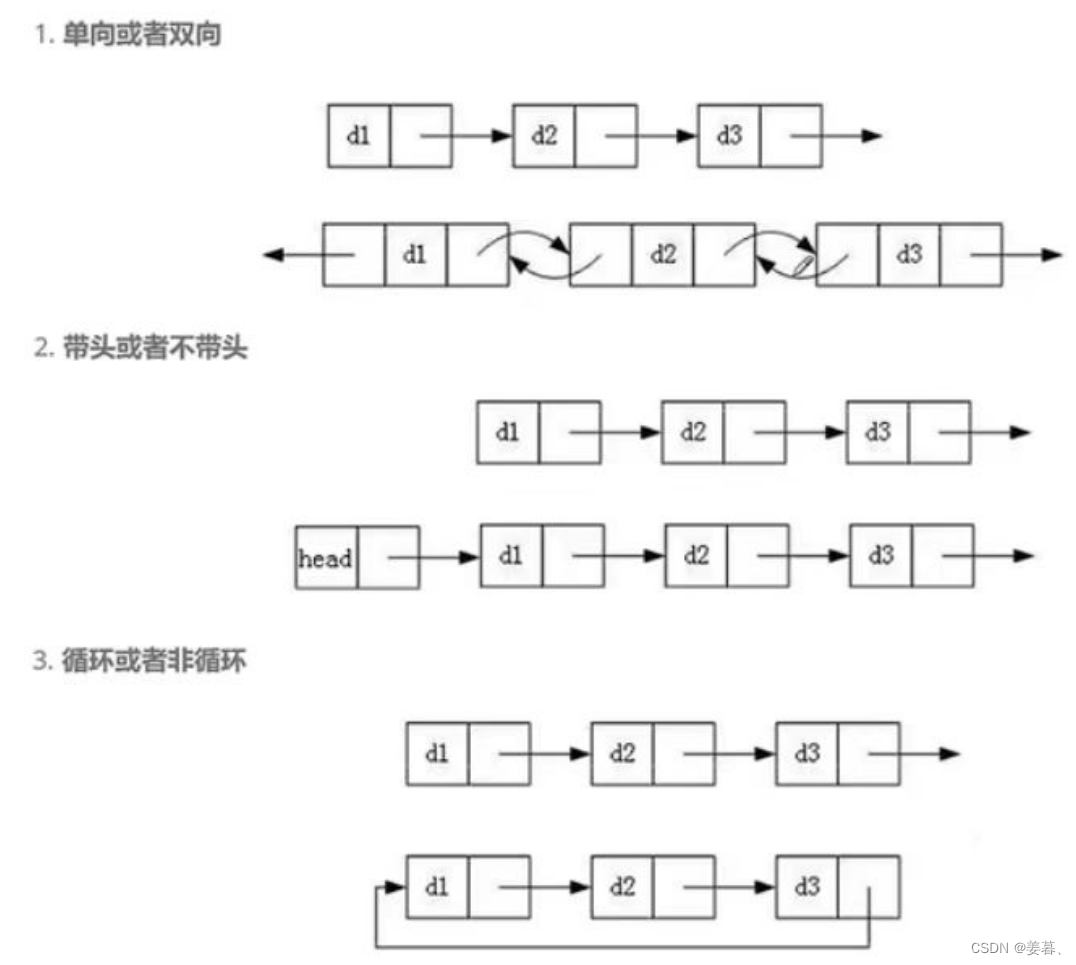
\includegraphics[width=0.7\textwidth]{链表1.png}
    \caption{链表} % 图片标题
    \label{fig:链表} % 图片标签,用于引用
\end{figure}

它的STL容器是$list$(双向链表)和$forward\_list$(单向链表)。比较简单,请自行去查阅相关文档:

\url{https://zh.cppreference.com/w/cpp/container/list}

\textbf{队列(Queue)}:队列是一种线性数据结构,它按照\textbf{先进先出}的原则进行操作。队列有两个基本操作,分别是\textbf{入队}和\textbf{出队}。入队操作是在队列的末尾添加一个元素,而出队操作是从队列的头部移除一个元素。队列有两个端点,队头和队尾,队头是队列的第一个元素,出队操作发生的地方,队尾是队列的最后一个元素,入队操作发生的地方。通常情况下,\textbf{不允许随机访问}队列中的元素,只能访问队头元素。
队列在\textbf{多任务处理、打印任务管理、缓冲处理}等场景中有广泛应用,它帮助维持操作的顺序和流程控制。
(很常用)
\begin{figure}[H]
    \centering
    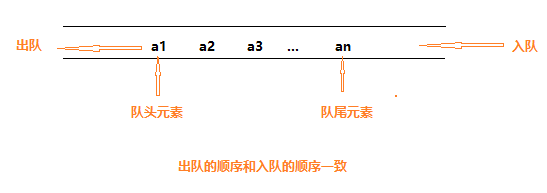
\includegraphics[width=0.7\textwidth]{队列1.png}
    \caption{入队和出队操作} % 图片标题
    \label{fig:入队和出队操作} % 图片标签,用于引用
\end{figure}
\begin{figure}[H]
    \centering
    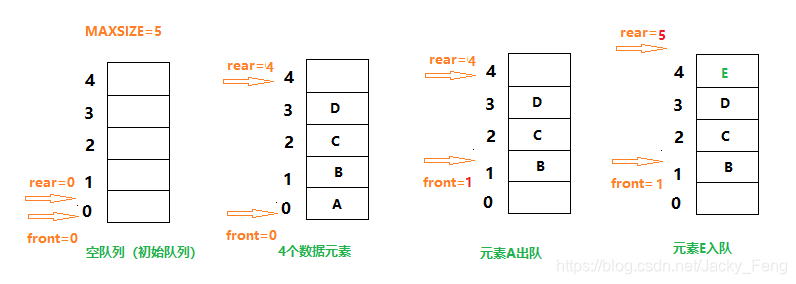
\includegraphics[width=0.7\textwidth]{队列2.png}
    \caption{队列实现方式} % 图片标题
    \label{fig:队列实现方式} % 图片标签,用于引用
\end{figure}

它的STL容器是$deque$,基于双向队列,C++还实现了3种容器适配器:
$stack$(堆栈),$queue$(单向队列),$priority\_queue$(优先队列),相较于$deque$,我们更常用$queue$
进行队列操作。
具体用法,请自行查阅相关文档:

\url{https://zh.cppreference.com/w/cpp/container/deque}

\url{https://zh.cppreference.com/w/cpp/container/queue}

\textbf{优先队列(Priority Queue)}:优先队列是一种特殊的队列,它允许插队的出现,可以根据“重要性”对队中元素进行排序。
优先队列的实现原理是每个元素都有一个优先级,优先级越高,元素越容易被取出。
优先队列的应用场景有很多,如任务调度、排序、搜索等。

\begin{figure}[H]
    \centering
    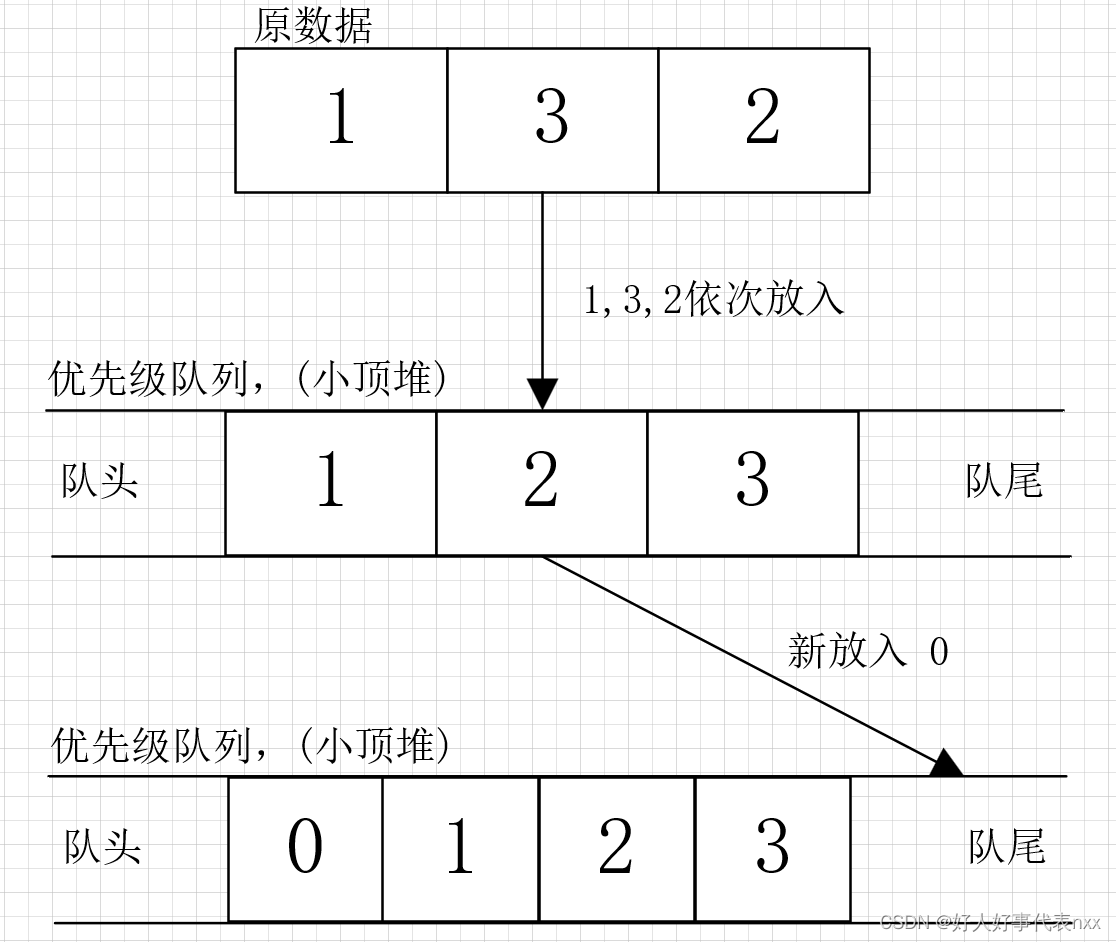
\includegraphics[width=0.7\textwidth]{优先队列1.png}
    \caption{优先队列} % 图片标题
    \label{fig:优先队列} % 图片标签,用于引用
\end{figure}

它的实现是容器适配器$priority\_queue$,
具体用法,请自行查阅相关文档:

\url{https://zh.cppreference.com/w/cpp/container/priority_queue}


\textbf{堆栈(Stack)}:堆栈是一种线性数据结构,它按照\textbf{先进后出}的原则进行操作。堆栈有两个基本操作,分别是\textbf{压栈}和\textbf{弹栈}。压栈操作是在堆栈的顶部添加一个元素,而弹栈操作是从堆栈的顶部移除一个元素。堆栈有两个端点,栈顶和栈底,栈顶是堆栈的顶部,压栈操作发生的地方,栈底是堆栈的底部,弹栈操作发生的地方。
堆栈在\textbf{函数调用、表达式求值、回溯、计算器、括号匹配、迷宫寻路}等场景中有广泛应用。

\begin{figure}[H]
    \centering
    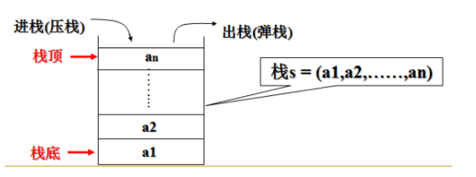
\includegraphics[width=0.7\textwidth]{堆栈1.png}
    \caption{压栈和弹栈操作} % 图片标题
    \label{fig:入队和出队操作} % 图片标签,用于引用
\end{figure}
\begin{figure}[H]
    \centering
    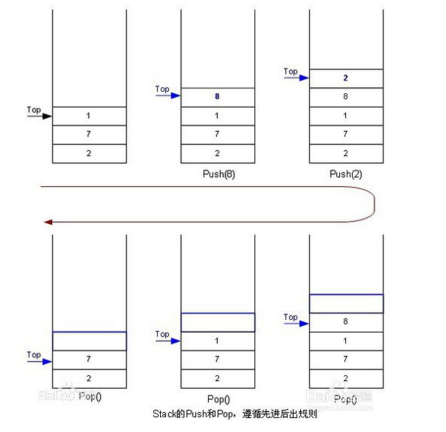
\includegraphics[width=0.7\textwidth]{堆栈2.png}
    \caption{堆栈实现方式} % 图片标题
    \label{fig:队列实现方式} % 图片标签,用于引用
\end{figure}

它的实现是容器适配器$stack$,
具体用法,请自行查阅相关文档。
\url{https://zh.cppreference.com/w/cpp/container/stack}

\textbf{树(Tree)}:树是一种非线性数据结构,它是由节点和边组成,节点之间存在着一种特定的关系。树的种类很多,如二叉树、二叉搜索树、AVL树、红黑树、B树、B+树、B*树等。
\begin{figure}[H]
    \centering
    \includegraphics[width=0.7\textwidth]{树1.png}
    \caption{树的逻辑图(了解即可)} % 图片标题
    \label{fig:队列实现方式} % 图片标签,用于引用
\end{figure}

\begin{figure}[H]
    \centering
    \includegraphics[width=0.7\textwidth]{树2.png}
    \caption{树的示意图} % 图片标题
    \label{fig:队列实现方式} % 图片标签,用于引用
\end{figure}

\textbf{堆(Heap)}:堆是一种特殊的树,它是一个\textbf{完全二叉树},即除叶节点外,其他的每个节点都有两个子节点。
每个节点都有一个值,并且每个节点\textbf{都大于或等于其子节点}(这是最大堆max-heap,类似的,还有最小堆min-heap)。堆的应用场景有很多,如排序、优先队列、图算法、堆排序等。

\begin{figure}[H]
    \centering
    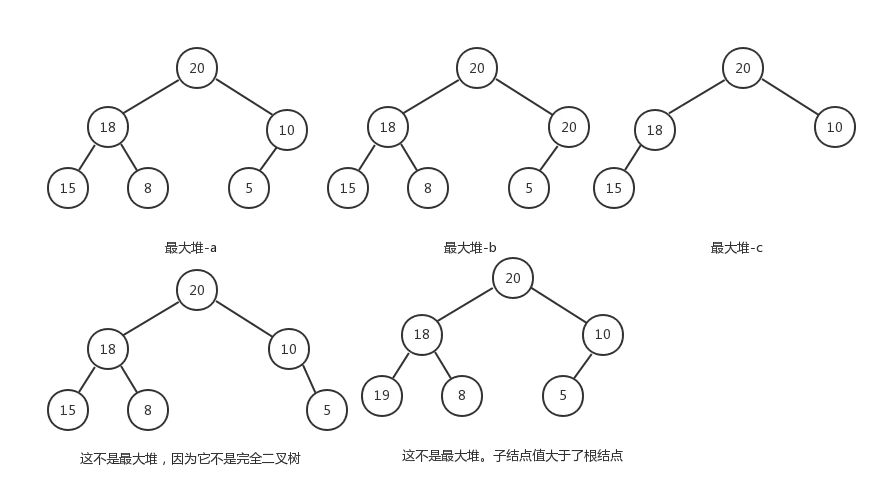
\includegraphics[width=0.7\textwidth]{最大堆.png}
    \caption{最大堆的示意图} % 图片标题
    \label{fig:最大堆} % 图片标签,用于引用
\end{figure}

\begin{figure}[H]
    \centering
    \includegraphics[width=0.7\textwidth]{堆1.png}
    \caption{最大堆和最小堆} % 图片标题
    \label{fig:最大堆和最小堆} % 图片标签,用于引用
\end{figure}

优先队列就是根据这个原理实现的,它是一种特殊的堆,具有\textbf{快速查找}的特性。他通过对于每个任务的重要程度进行编号,并将编号大的任务放在堆的顶部,这样就可以快速的找到重要的任务。
由于堆的排序算法非常快,可以实现更快速的任务调整,因此优先队列被广泛地应用于\textbf{任务管理}中。

优先队列的STL容器是$priority\_queue$。

具体用法,请自行查阅相关文档:

\url{https://zh.cppreference.com/w/cpp/container/priority_queue}

\textbf{映射(Map)}:映射是一种关联容器,它是一个\textbf{键值对}的集合,其中每个键都是唯一的,值可以重复。
映射的实现原理是通过哈希表(或红黑树)实现的,因此,查找、插入、删除操作的时间复杂度都是$O(1)$(或$O(logN)$)。

\textbf{红黑树(Red-Black Tree)}是一种随机查找速度比较快的\textbf{平衡二叉树}\footnote{
    平衡二叉树,也叫AVL树,它或者是一颗空树,或者具有以下性质的二叉排序树:它的左子树和左子树的高度之差(平衡因子)的绝对值不超过1,且它的左子树和右子树都是一颗平衡二叉树}
,他的查找、插入、删除操作的时间复杂度都是$O(logN)$ \footnote{
    O(logN)表示时间复杂度,N是问题的规模,O表示运行消耗时间的上界
}。

\textbf{哈希表(HashTable)}是一种\textbf{散列表},它通过\textbf{哈希函数}将键映射到值。
由于其使用计算来查找,因此,查找操作的时间复杂度都是$O(1)$
\footnote{常数的时间复杂度意味着不管问题的规模如何,
对于同一个长度的HashTable,算法的运行时间都不会随着问题的规模增加而增长。}。
但是哈希表的建立比较困难,需要消耗很多资源。
而且存储长度有限,当元素过多时,哈希表的性能会下降。当哈希表满时,需要执行\textbf{再散列(Rehashing)},解决\textbf{哈希冲突(Hash Collision)}问题,
这个过程需要消耗大量时间。

两者各有优劣,在实际应用中,需要根据具体问题选择。
红黑树型映射的STL容器是$map$,哈希表型映射的STL容器是$unordered\_map$,
具体用法,请自行查阅相关文档:

\url{https://zh.cppreference.com/w/cpp/container/map}

\subsubsection{STL的迭代器}

\textbf{迭代器},是一种检查容器内元素并遍历元素的数据类型,通常用于对C++中各种容器内元素的访问,
但不同的容器有不同的迭代器,初学者可以将迭代器理解为一个可以\textbf{自动向后移动的指针}。

常用的可迭代的容器有:

\begin{enumerate}
    \item 序列容器:$array$、$vector$、$deque$、$list$、$forward\_list$等
    \item 关联容器:$set$、$map$、$multimap$等
\end{enumerate}

$queue$、$stack$、$priority\_queue$是容器适配器,必须满足一定规则,没有迭代器。

对于可迭代容器,一般可以使用.begin()和.end()方法获取迭代器,.begin()方法返回指向第一个元素的迭代器,
.end()方法返回指向最\textbf{后一个元素的迭代器的下一位置}。
使用迭代器,可以方便的对容器内元素进行遍历,例如:

\begin{tcode}
std::vector<int> vec{1,2,3,4,5,6,7,8,9,0};
for(auto it = vec.begin();it != vec.end();++it){
    std::cout << *it << std::endl;
}
\end{tcode}

也可以简写为:

\begin{tcode}
for (auto it: vec) {
    std::cout << it << std::endl;
}
\end{tcode}

还可以使用迭代器对容器内元素进行修改,例如:

\begin{tcode}
std::vector<int> vec{1, 2, 3, 4, 5, 6, 7, 8, 9, 0};
vec.erase(vec.begin()+5);//删除第6个元素
vec.erase(vec.begin()+5,vec.end());//删除第6个元素之后的所有

std::vector<int> vec1{1, 2, 3, 4, 5, 6, 7, 8, 9, 0};
std::iter_swap(vec1.begin(),vec1.begin()+1);//交换第一个和第二个元素

std::vector<int> vec2{1, 2, 3, 4, 5, 6, 7, 8, 9, 0};
//此函数需要头文件<algorithm>
std::sort(vec2.begin(),vec2.end(),[](int& a,int& b){
    return a>=b;
});

//此函数需要头文件<algorithm>
//删除大于5的元素
auto newVec = std::remove_if(vec2.begin(),vec2.end(),[](int& a){
    return a>5;
});
\end{tcode}

我们不会使用十分复杂的迭代器,感兴趣的同学可以看一下cppreference的相关文档:

\url{https://zh.cppreference.com/w/cpp/iterator}

\textbf{迭代器失效}:迭代器失效指的是迭代器因为某些操作而不再指向原来的元素,
或者不再保持有效的状态,这样的迭代器如果继续使用,可能会导致未定义行为,包括程序崩溃。
通俗的理解就是,当你对容器进行了操作时,更改了容器的大小,但是迭代器仍然指向原来的位置,
这样就会导致读取错误的内存,这就是迭代器失效。

\begin{tcode}
std::vector<int> vec={1,2,3,4,5,6,7,8,9,10};
for(auto it = vec.begin(); it!= vec.end(); ++it){
    if(*it%2==0){
        vec.erase(it);
    }
}
\end{tcode}

看上面的代码,当执行到vec.erase(it)时,it已经失效,因为执行了erase之后,
vec的大小发生了变化,这导致了迭代器失效。

在实践过程中, 在下面的几种情况下,迭代器会失效,需要\textbf{避免}出现:
\begin{enumerate}
    \item 当执行erase方法时,指向删除节点的迭代器全部失效,指向删除节点之后的全部迭代器也失效
    \item 当进行push\_back\(\)方法时,end操作返回的迭代器肯定失效。
    \item 当插入\(push_back\)一个元素后,capacity返回值与没有插入元素之前相比有改变,
    则需要重新加载整个容器,此时first和end操作返回的迭代器都会失效。
    \item 当插入\(push_back\)一个元素后,如果空间未重新分配,指向插入位置之前的元素的迭代器仍然有效,但指向插入位置之后元素的迭代器全部失效。
\end{enumerate}

对于关联容器,使用迭代器时,删除一个键值对知识当前这个迭代器失效,别的迭代器不会受到影响,
这可能是由于底层使用红黑树实现的原因,但是实际应用中,仍然不应该冒这个风险,因此,
必须\textbf{坚决避免迭代器失效问题的发生}。

在具体的应用中,我们在使用迭代器遍历时,应该注意不要对容器进行增删操作,更不应该改变容器的大小。
可以将不需要的元素放在\textbf{容器的末尾}或者\textbf{记录下需要删除的迭代器},然后适时删除。例如:

\begin{tcode}
for(auto it = vec.begin(); it!= vec.end(); ++it){
    if((*it)%2==0){
        its.push_back(it-vec.begin());
    }
}

int i=0;
for(auto it : its){
    vec.erase(vec.begin()+it-i);
    i++;
}
}
\end{tcode}

这种方法,非常\textbf{不优雅},因此,\textbf{不要使用}。

\textbf{更多的用法等待着同学们自己去探索!}

\subsubsection{系统级内存运行逻辑}

C++是一个十分灵活的编程语言,其中指针的概念为程序员们提供了直接操纵内存的能力。
指针的使用使得程序员可以自由的操作内存,但是也带来了一些安全性和复杂性问题。
因此,了解程序运行的底层逻辑,对于理解C++至关重要,对于提高程序效率举重若轻,下面我们来看看C++的内存运行逻辑。

\begin{figure}[H]
    \centering
    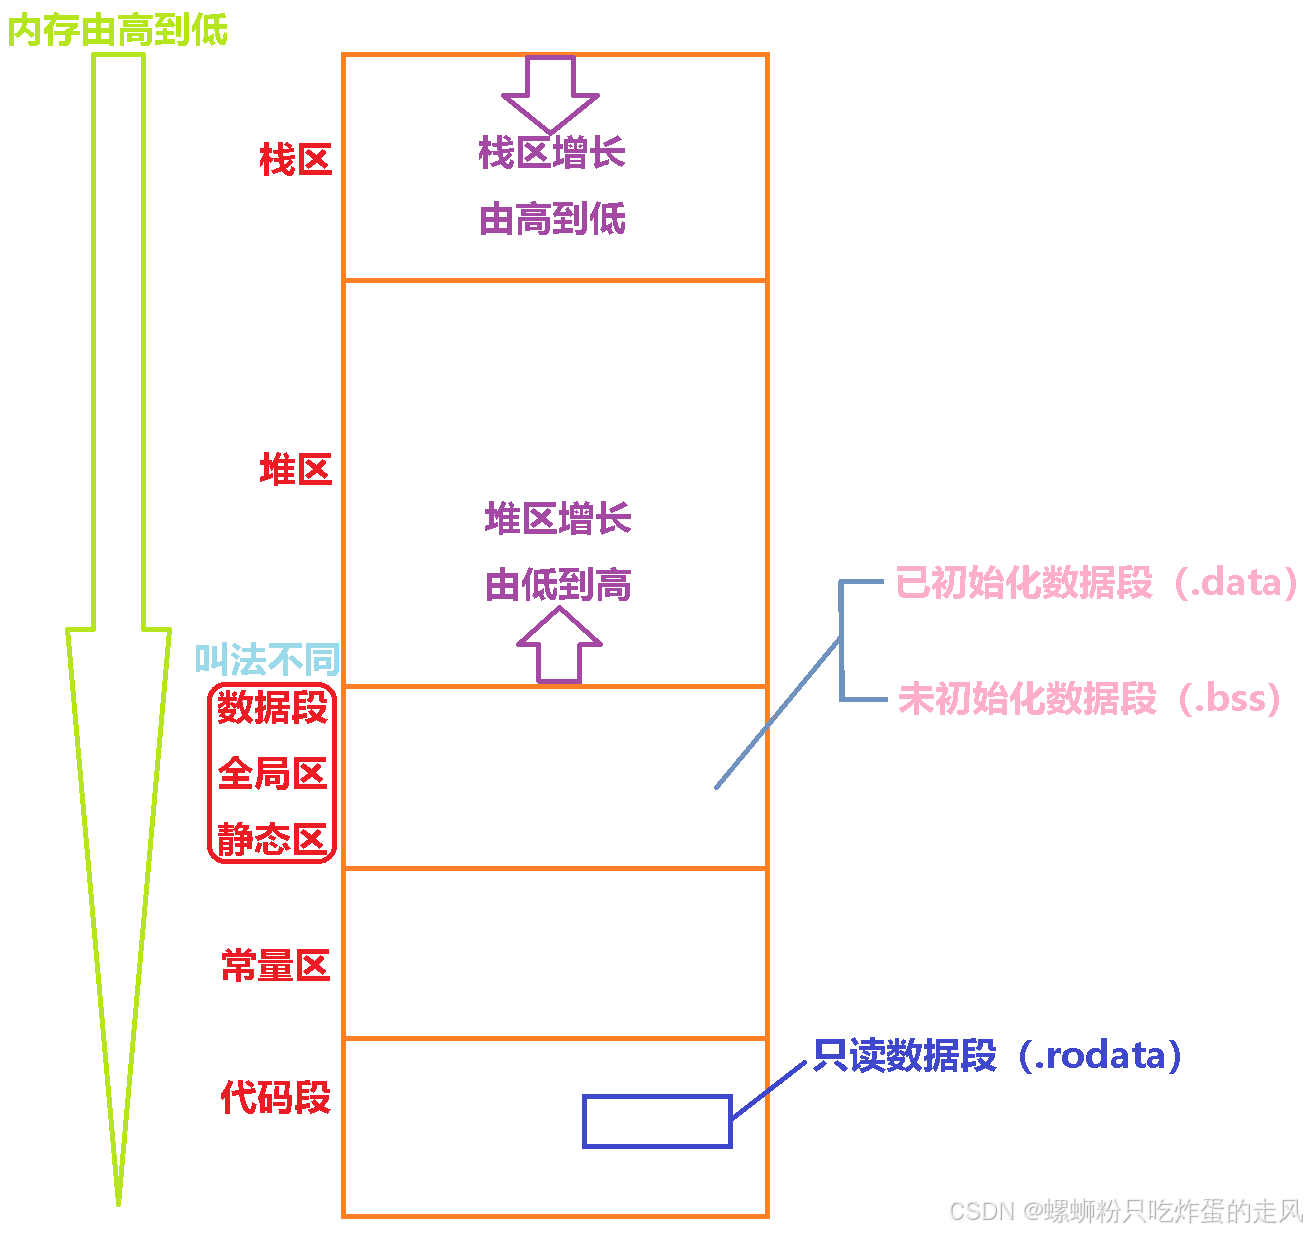
\includegraphics[width=0.7\textwidth]{系统内存.png}
    \caption{系统内存分区} % 图片标题
    \label{fig:内存分区} % 图片标签,用于引用
\end{figure}

如图\ref{fig:内存分区},系统内存分为\textbf{代码区、常量区、全局/静态变量区、堆区、栈区等几个部分}。

\textbf{代码区和常量区}是存放程序代码和常量数据的区间一般不作区分,这里的数据是只读的,其中存储着一些在编译过程前就可以确定的数据内容
,如代码、$constexpr$修饰的变量、$const$修饰的在预编译期可以确定的值等,
一些字面常量如"Hello World!",也存储于其中。程序在常量区中只能读取数据。

\textbf{全局/静态变量区}是存放全局/静态变量的区间,全局变量在程序运行前就已经分配了内存,静态变量在程序运行前也已经分配了内存。
但是静态变量的生命周期比全局变量长,它在程序运行结束后才释放内存。

\begin{enumerate}
    \item 全局变量:在函数外部定义的变量,它们具有全局作用域。
    \item 静态全局变量:在函数外部定义并用 $static$ 关键字修饰的变量,它们具有内部链接属性,即它们只能在定义它们的文件内部可见。
    \item 静态局部变量:在函数内部定义并用 $static$ 关键字修饰的变量,它们在函数调用结束后仍然存在,并且保持它们的值。
    \item 类静态成员变量:在类定义中使用 $static$ 关键字声明的成员变量,它们属于类而不是类的任何一个实例。
\end{enumerate}

解释一下\textbf{静态}:
\begin{enumerate}
    \item 生命周期上,静态变量在程序开始运行前或类的实例化之前就已经分配了内存,在程序运行结束后才释放内存。地址不会发生变化,就静静“躺”在静态变量区,直到程序结束。
    \item 相对于$new$的动态分配,可以让程序员选择什么时候分配和释放内存,而$static$变量则是一直存在的,直到程序结束。
    \item 静态全局变量也具有全局作用域,他与全局变量的区别在于如果程序包含多个文件的话,他作用于定义它的文件里,不能作用到其他文件里,即被$static$关键字修饰过的变量具有文件作用域。这样即使两个不同的源文件都定义了相同的静态全局变量,他们也是不同的变量。这点于全局变量不同。
\end{enumerate}

\textbf{堆区}:堆区是由程序员手动分配和释放的内存,堆区的分配和释放由\textbf{程序员控制},程序员可以通过$new$和$delete$操作符来分配和释放内存。

在大小上,堆区的大小相对于栈区是很大的,因此可以存储更多的数据。初次之外,堆区是由程序员全权负责管理的,程序员必须小心管理堆区的分配和释放,确保程序的正确性和安全性,一般使用\textbf{智能指针}和$nullptr$判断提高程序的稳定性。
但与此同时,堆区也提供了更为灵活的编程和数据传递模式,可以参考下面的例子:
\begin{tcode}
std::vector<int>* func(){
    std::vector<int>* a = new std::vector<int>({1,2,3,4});
    std::vector<int> b{1,2,3,4};
    return a;//return &b;
    //换成return &b;之后再试试呢?
}

int main() {
    auto vecPtr = func();
    return 0;
}
\end{tcode}

\textbf{栈区}:栈区是由\textbf{编译器自动分配和释放的内存},栈区的分配和释放都是编译器\textbf{自动完成}的,程序员\textbf{无法直接控制}栈区的分配和释放。
栈区存储数据的优势在于\textbf{快速},但是也有一些缺点,比如栈区的大小是有限的,因此在函数调用层次过深时,可能会出现栈溢出。
栈区的大小一般是$2MB$,因此栈区的大小是有限制的,如果函数调用层次过深,可能会出现栈溢出。

\textbf{系统内存管理}:系统内存管理是操作系统的工作,它负责分配和释放系统内存,其中操作系统会自行决定栈内存,下面我们讨论一下栈区的操作。

在栈内存中,数据存储在系统栈中,只有一个开口,数据只能从栈顶入栈和出栈。在切换代码的\textbf{作用域}时,上一个作用域的数据会被新的数据压在栈的下方,
这些数据将不能被当前的程序进程所读取,直到当前的这些数据被弹出栈。
栈内存的设计是十分精妙的,它可以有效的解决内存分配和释放的问题,亦可以实现函数的层次调用,作为一名C++程序员,我们要理解透彻栈内存的运行逻辑。

\textbf{函数递归的底层原理}:函数递归是一种非常有趣的编程技巧,它可以让程序员以一种\textbf{迭代}的思想来理解和编写代码。

\begin{figure}[H]
    \centering
    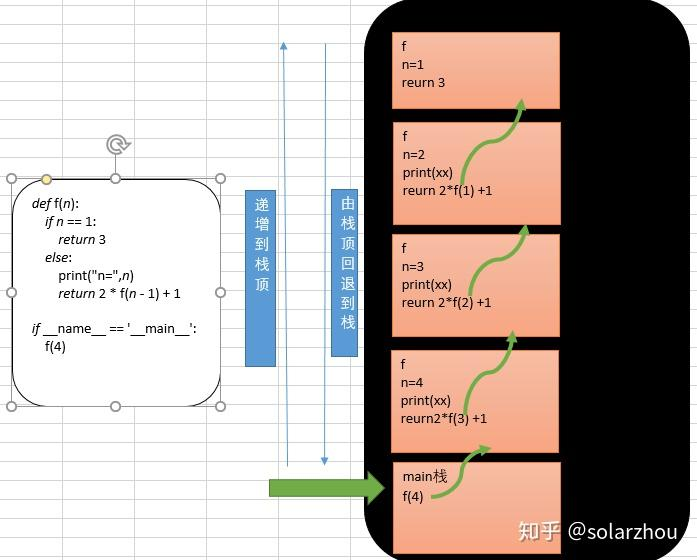
\includegraphics[width=0.7\textwidth]{栈递归.jpg}
    \caption{函数递归调用栈} % 图片标题
    \label{fig:栈递归} % 图片标签,用于引用
\end{figure}

在函数调用时,新的函数的栈帧会被压入栈中(称为栈帧),从而覆盖掉原来的\textbf{栈帧},当函数返回时,栈帧会被弹出栈。
露出原来的函数栈帧。当函数调用自身时,会形成一个\textbf{递归调用栈}。

需要注意的是,栈内存的大小是有限制的,当函数调用层次过深时,会出现栈溢出。

\subsubsection{C++的多线程}

多线程技术是C++中非常重要的特性之一,它可以让程序员以更高的并发性和速度运行程序。使用多线程可以提高程序的运行效率,丰富程序的运行逻辑,实现许多单线程所不能实现的功能。
在C++中,提供了$<threaed>$库来实现多线程的功能。

\textbf{多线程的原理}:多线程是指在同一程序中同时运行多个线程来完成不同的任务,以提高资源利用率和程序响应速度。
硬件条件上,多线程需要CPU支持多核处理或多任务处理,以及足够的内存和处理器资源。在多线程编程过程中,可能遇到一些问题,
包括线程同步、死锁、竞态条件等,这些问题可能导致程序运行不稳定、性能下降甚至系统崩溃。
因此,在设计多线程程序时,需要充分考虑线程之间的\textbf{协作与互斥},合理分配资源,以保障程序的正确性和高效性。
在多线程之中,有两种主要的设计模式,即\textbf{阻塞}和\textbf{非阻塞}。

\begin{enumerate}
    \item \textbf{阻塞}:在阻塞模式下,线程在等待某个事件的发生,如等待IO操作完成、等待子进程结束等。
当某个事件发生时,线程会被唤醒,并开始执行。

    \item \textbf{非阻塞}:在非阻塞模式下,线程在等待某个事件的发生,但不会被挂起,而是继续执行后续代码。
当某个事件发生时,线程会被通知,并开始执行。
\end{enumerate}


\textbf{创建线程}:
C++11中引入的$<thread>$库提供了多线程的支持,它提供了$std::thread$类来创建和管理线程:

\begin{tcode}
用法:std::thread ThreadName(函数指针,[参数]);
实例:
void function1(){for(int i=0;i<1000;i++);}
void function2(int a,int &b){for(int i=0;i<1000;i++);}
int main() {
    std::thread th1(function1);
    int a=0, b=0;
    std::thread th1(function1,a,std::ref(b));
    return 0;
}
\end{tcode}

如果你想要在线程中传递参数,可以直接传递参数,也可以使用引用传递参数,引用传参的时候需要使用$std::ref()$函数。
你也可以使用$join()$方法使主线程等待所有线程结束,
$detach()$方法将线程分离,这样主线程就不会等待主线程结束而结束。

\textbf{线程同步和互斥锁}:
多线程程序的稳定性和互斥锁是多线程编程中经常遇到的问题。请参考下面的例子:
\begin{tcode}
int i=0;
void function1(){
    for(int j=0;j<100000;j++)
        i++;
}

int main() {
    std::thread th1(function1);
    for(int j=0;j<100000;j++)
        i++;
    if(th1.joinable())
        th1.join();
    std::cout << i;
    return 0;
}
\end{tcode}
在程序的运行过程中,$i$的值可能是$0$,也可能是$200000$,这取决于线程的调度。
当两个线程同时拿到$i$的地址时,同时对i进行写入操作,两者就会出现线程同步问题。
那怎么解决这个问题呢?$std::mutex$和$std::lock\_guard$为我们提供了解决方案——互斥锁。是解决线程同步问题的两种方法。
$mutex$是一种同步机制,它可以保证同一时刻只有一个线程对共享资源进行访问。
$lock\_guard$是一个智能指针,它可以自动获取互斥锁,并在离开作用域时自动释放互斥锁。

\begin{tcode}
#include <iostream>
#include <thread>
#include <mutex>

int i=0;
std::mutex lock;
void function1(){
    for(int j=0;j<100000;j++){
        lock.lock();
        i++;
        lock.unlock();
    }
}

int main() {
    std::thread th1(function1);
    for(int j=0;j<100000;j++){
        lock.lock();
        i++;
        lock.unlock();
    }
    if(th1.joinable())
        th1.join();
    std::cout << i;
    return 0;
}
\end{tcode}
发现程序的稳定性已经得到提高,在多次运行过程中,$i$的值始终是$200000$。这一点在多线程编程过程中非常重要,是所有程序员的必修课。
但是,这是又产生了一个新的问题,那就是程序员还是需要进行互斥锁的手动管理,这无疑会降低程序开发的效率。
类似于智能指针的,C++11中引入了$std::lock\_guard$来自动管理互斥锁,它可以自动获取互斥锁,并在离开作用域时自动释放互斥锁。

\begin{tcode}
#include <iostream>
#include <thread>
#include <mutex>

int i=0;
std::mutex lock;
void function1(){
    for(int j=0;j<100000;j++){
        std::unique_lock<std::mutex> Autolock;
        i++;
    }

}

int main() {
    std::thread th1(function1);
    for(int j=0;j<100000;j++){
        std::unique_lock<std::mutex> Autolock;
        i++;
    }

    if(th1.joinable())
        th1.join();
    std::cout << i;
    return 0;
}
\end{tcode}
程序测试成功,$i$的值始终是$200000$。

\textbf{死锁}:在使用互斥锁的时候,如果多个线程都在\textbf{等待对方释放锁},就会出现死锁。请看下面的例子:

\begin{tcode}
int i=0;
std::mutex lock1;
std::mutex lock2;
void function1(){
    for(int j=0;j<100000;j++){
        lock1.lock();
        lock2.lock();
        i++;
        lock2.unlock();
        lock1.unlock();
    }
}

int main() {
    std::thread th1(function1);
    for(int j=0;j<100000;j++){
        lock2.lock();
        lock1.lock();
        i++;
        lock2.unlock();
        lock1.unlock();
    }

    if(th1.joinable())
        th1.join();
    std::cout << i;
    return 0;
}

\end{tcode}

在这个例子中,两个线程都在等待对方释放锁,导致死锁。在设计时,尽量使得不同的互斥锁以相同的顺序被获取和释放,可以降低死锁的概率。

\textbf{原子变量}:在C++11中,引入了原子类型$std::atomic$,它可以保证变量的原子性,即在读写操作时,其他线程只能看到该变量的\textbf{已修改}值。
使用这种方式,可以增强程序的可读性。原子变量也不需要使用互斥锁进行同步,它可以自动保证原子性。

\textbf{条件变量}:条件变量($Condition Variable$)是一种用于线程同步的机制,通常与互斥锁($Mutex$)一起使用。条件变量提供了一种线程间的通信机制,允许一个线程等待另一个线程满足某个条件后再继续执行。

我们通过一个例子来简单理解一下这个问题:

现在小明在一张桌子上放一个苹果,而旁边有一群蒙着眼睛的人,因为他们的眼睛被蒙着,
他们如果想拿到这个苹果,就会时不时来桌子前摸一摸看看桌子是否有苹果,并且谁来桌子前摸苹果是无序的,
这时的场面就很混乱,小明一看不行,于是小明就桌子上放了个铃铛,并且组织需要苹果的人排好队,
有苹果小明就会摇响铃铛,排在第一个的人就拿走苹果,然后如果还想要苹果就到队尾排队等待
。此时混乱的场面就显得井然有序了。在本故事中,小明就是操作系统,苹果就是临界资源,
一群蒙着眼睛都人就是多线程,铃铛就是条件变量,排队就是实现同步,摇响铃铛就是唤醒线程。

使用条件变量主要是因为它们提供了在多线程编程中一种有效的同步机制。
当多个线程需要\textbf{等待某个特定条件}成立才能继续执行时,条件变量就显得尤为重要。
通过条件变量,线程可以安全地进入等待状态,直到被其他线程显式地唤醒或满足等待的条件。
这有助于避免线程的\textbf{无谓轮询或忙等待},提高了系统的响应能力和效率。
\textbf{注意}:在使用条件变量时,必须确保与\textbf{互斥锁}一起使用,以\textbf{避免竞态条件}的发生。

下面介绍一下$condition\_variable$的用法:

调价变量的使用大致可以分为两个大的功能,即$notify$和$wait$。

\begin{tcode}
std::condition_variable condition;//声明
condition.notify_all();//通知所有等待线程
condition.notify_one();//通知第一个接收的等待线程

std::unique_lock<std::mutex> Lock(mtx);
condition.wait(Lock);//等待条件成立
condition.wait(Lock,[](){return true;});//等待条件和第二个参数同时为true
\end{tcode}

\textbf{消费者-生产者模型},是多线程编程中经常使用的模型。
生产者-消费者模型是指多个生产者线程和多个消费者线程之间通过一个共享的缓冲区进行通信。
生产者线程负责生产数据,并将其放入缓冲区;消费者线程则负责从缓冲区中取出数据进行消费。
生产者和消费者之间通过一个\textbf{条件变量}进行同步,以保证缓冲区中的数据不会被消费者线程消费完。

\begin{tcode}
#include<iostream>
#include<thread>
#include<mutex>
#include<condition_variable>
#include<queue>
#include<functional>

std::mutex lock;
std::condition_variable cv;
std::queue<std::function<void()>> taskQueue;
void consumer(){
    while(1){
        std::unique_lock<std::mutex> Lock(lock);
        cv.wait(Lock,[&](){
            return !taskQueue.empty();
        });
        auto task = taskQueue.front();
        task();
        taskQueue.pop();
        Lock.unlock();
    }
}

void producer(int i){
    auto func = [](int id){
        std::cout << "task" << id << " is running!" << std::endl;
    };
    std::function<void()> task = std::bind(func,i);
    {
        std::unique_lock<std::mutex> Lock(lock);
        taskQueue.push(task);
    }
    cv.notify_one();
    std::this_thread::sleep_for(std::chrono::seconds(1));
}

int main(int argc,char** argv){
    std::thread consumer_thread(consumer);
    for(int i=0;i<100;i++){
        producer(i);
    }

    if(consumer_thread.joinable())
        consumer_thread.join();
    return 0;
}
\end{tcode}

\textbf{线程池}:线程池是一种常用的技术,它可以提高程序的并发性,减少线程创建和销毁的开销,并可以有效的利用系统资源。
下面是一种线程池的实现方式,尝试一下把它看懂吧!

\begin{tcode}
#include <iostream>
#include <thread>
#include <mutex>
#include <condition_variable>
#include <functional>
#include <vector>
#include <queue>

class ThreadPool
{
private:
    std::vector<std::thread> threads;
    std::queue<std::function<void()>> tasks;
    std::mutex mtx;
    std::condition_variable condition;
    bool stop;

public:
    ThreadPool(int numThreads):stop(false) {
        for (int i = 0; i < numThreads; i++) {
            threads.emplace_back([this] {
                while (1) {
                    std::unique_lock<std::mutex> lock(mtx);
                    condition.wait(lock, [this] {
                        return !threads.empty() || stop;
                    });
                    if (stop && tasks.empty())
                        return;

                    auto task = std::move(tasks.front());
                    tasks.pop();
                    lock.unlock();
                    task();
                }
            });
        }

    }

    ~ThreadPool() {
        {
            std::unique_lock<std::mutex> lock(mtx);
            stop = true;
        }
        condition.notify_all();
        for (auto& iter : threads) {
            iter.join();
        }
    }

    template<class F, class ...Args>
    void enqueue(F&& f, Args&&... args) {
        std::function<void()> task =
                std::bind(std::forward<F>(f), std::forward<Args>(args)...);
        {
            std::unique_lock<std::mutex> lock(mtx);
            tasks.emplace(std::move(task));
        }
        condition.notify_one();
    }

};

int main() {
    ThreadPool Pool(4);
    for (int i = 0; i < 100; i++) {
        Pool.enqueue([i] {
            std::cout << "task" << i << "is running!" << std::endl;
            std::this_thread::sleep_for(std::chrono::seconds(1));
            std::cout << "task" << i << "has finished!" << std::endl;
        });
    }

    return 0;
}
\end{tcode}

\section{编译原理与CMake基础}

在实际工程中,编译器的选择往往是影响编译速度的关键因素。CMake是一种跨平台的编译工具,它可以用来管理工程的构建,自动生成makefile或project文件,并提供方便的接口来调用编译器、链接器等工具。

\subsection{C++的编译过程}

C++的编译过程可以分为以下几个步骤:

\begin{enumerate}
    \item \textbf{预处理}(Preprocessing):预处理器会对源代码进行预处理,将所有的宏定义、条件编译等操作展开,生成一个新的源文件。
    \item \textbf{编译}(Compilation):编译器会将预处理后的源文件编译成汇编语言。
    \item \textbf{汇编}(Assemble):汇编器会将汇编语言代码转换成机器语言。
    \item \textbf{链接}(Linking):链接器会将多个目标文件和库文件链接成一个可执行文件。
\end{enumerate}

\begin{figure}[H]
    \centering
    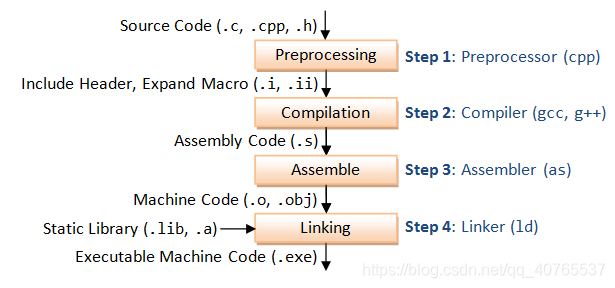
\includegraphics[width=0.7\textwidth]{编译流程.png}
    \caption{C++编译过程} % 图片标题
    \label{fig:编译} % 图片标签,用于引用
\end{figure}

\textbf{预编译}:
预编译器会对源代码进行预处理,将所有的宏定义、条件编译等操作展开,生成一个新的源文件。
预编译器的作用主要是对源代码进行预处理,以便于编译器进行编译。
比如说,对于一个头文件引用$\#include<iostream>$,预编译器会将其展开为头文件的源代码,
生成一个新的源文件,然后再进行编译。对于头文件,预编译器只会进行一次,而对于源文件,
预编译器会在每个源文件编译前进行一次。在代码中的宏定义$\#define$会在预编译时进行字符串替换,
而条件编译$\#if$则会根据条件是否成立来决定是否展开代码。
只有理解了这些,才能真正理解宏和条件编译的作用。

在C/C++中有一些预定义的宏,可以拿来直接用,如:
\begin{tcode}
__FUNTION__  获取当前函数名 
__LINE__ 获取当前代码行号 
__FILE__ 获取当前文件名 
__DATE__ 获取当前日期 
__TIME__ 获取当前时间
__STDC_VERSION__  获取当前编译器的版本
\end{tcode}

\textbf{编译}:
编译器会将预处理后的源文件编译成汇编语言。
编译阶段进行语法分析、词法分析和语义分析,并且将代码优化后产生相应的汇编代码文件(ASCLL文件),
即.s 文件。这个过程是整个程序构建的核心部分,也是最复杂的部分之一。

\textbf{汇编}:
通过不同平台(Windows、Linux)的汇编器将汇编代码翻译成机器码,即生成二进制可重定向文件(.o)。
任何一个源文件在进行编译阶段的时候会去产生\textbf{符号表},符号表中存放的就是程序所产生的符号
(例如:函数名,变量名等),我们的编译阶段是不会去给符号分配正确的地址。这些\textbf{符号}都没有被分配地址,
因此.o文件没有经过链接是无法执行的。

\textbf{链接}:
链接器会将多个目标文件和库文件链接成一个可执行文件。
链接器的作用是将多个目标文件和库文件链接成一个可执行文件,这个过程会将符号表中的符号分配正确的地址,
并将各个目标文件中的代码和数据合并到一个可执行文件中。
简单来说,\textbf{连接就是将符号和数据进行整合,最终得到一个可以指定的文件。}

链接有两种方式:\textbf{静态链接}和\textbf{动态链接}。
相对应的,这两种链接方式所对应的库就称为\textbf{静态库}和\textbf{动态库}。

\textbf{静态库}:
静态库是编译好的目标文件,在链接时会被直接链接到可执行文件中。
静态库的优点是编译速度快,缺点是可执行文件体积大,因为它包含了所有程序需要的目标文件。

\textbf{动态库}:
动态库是运行时加载的库,在程序运行时才被加载到内存中。
动态库的优点是可执行文件体积小,缺点是运行速度慢,因为它需要在运行时加载。

\subsection{CMake}
从上面的介绍中,可以看出,编译过程是十分复杂的,错误的编译方式可能会导致编译失败,或者编译的程序无法正确运行。
为了告诉编译器如何编译我们的程序,工程师们开发了$makefile$,它是一种描述编译过程的脚本文件。
$makefile$的优点是简单易懂,缺点是不够灵活,工程师需要写大量的$makefile$,并且需要手动管理。
在这种困境下,CMake应运而生。

\textbf{CMake}是一种跨平台的编译工具,它可以用来管理工程的构建,自动生成$makefile$或$project$文件,
并提供方便的接口来调用编译器、链接器等工具。$CMake$的优点是简单易用,它会根据工程的结构自动生成$makefile$,
并且可以自动检测编译器、库的安装路径,使得工程师只需要关注工程的源代码即可。

CMake的使用十分简单,只需要在工程的根目录下创建一个$CMakeLists.txt$文件,然后在其中写入编译指令即可。
主要的工作内容有:

\begin{enumerate}
    \item \textbf{项目配置}:确定工程的名称、版本、作者、编译器、编译器版本、编译类型等。
    \item \textbf{添加文件}:添加工程需要编译的源文件和头文件,查找依赖包,并将其加入编译列表。
    \item \textbf{编译}:使用CMake提供的接口编译工程,生成重定向文件和库文件。
    \item \textbf{连接}:将重定向文件和库文件链接成可执行文件。
    \item \textbf{安装}:将可执行文件安装到指定目录。
\end{enumerate}

下面我们来逐个分析介绍一下CMake的使用方法:

\subsubsection{项目配置}
使用CMake的第一步是配置工程,首先需要创建一个$CMakeLists.txt$。
在$CMakeLists.txt$文件中,
我们需要指定工程的信息,如项目名称、编译器、编译器版本、编译选项等。需要强调的是,
$CMake$本身\textbf{不具有编译功能},它只是用来管理工程的构建,具体来说,是形成一套编译器可以“看懂”的文件
然后编译器根据这些文件进行编译。

常用的命令有:
\begin{tpython}
project(project_name)  # 设置项目名称
cmake_minimum_required(VERSION 2.8)  # 设置CMake的最低版本
set(CMAKE_CXX_COMPILER "g++")  # 设置编译器
set(CMAKE_CXX_FLAGS "-Wall -g")  # 设置编译选项
set(CMAKE_CUDA_COMPILER /usr/local/cuda-11.8/bin/nvcc) # 设置CUDA编译器路径
enable_language(CUDA)  # 启用CUDA语言
\end{tpython}
需要强调的是,$CMake$的指令(括号外)是不区分大小的。但是变量和值(括号内)是大小写\textbf{敏感}的。

后期还会使用到的一些指令:
\begin{tpython}
set(CMAKE_CUDA_COMPILER /usr/local/cuda-11.8/bin/nvcc) # 设置CUDA编译器路径
enable_language(CUDA)  # 启用CUDA语言
\end{tpython}

这里需要特别强调一下$set$指令,它可以设置变量的值,并可以用变量来代替值。
可以使用\textbf{宏}来读取$set$所设置的变量的值,如:
\begin{tpython}
message(STATUS ${CMAKE_CXX_COMPILER})  # 打印编译器路径
\end{tpython}

其中,$CMAKE\_CXX\_COMPILER$是$CMake$预定义的宏,表示编译器的路径,使用$\$\{\}$可以使用宏的值。
$CMake$中所有的配置过程都是在进行\textbf{宏}的配置,这里体现一种$set$两种用法的统一性,我们可以根据自己的需求来设置。

\subsubsection{添加文件}

在$CMakeLists.txt$文件中,我们需要添加工程需要编译的源文件和头文件,查找依赖包,并将其加入编译列表。

常用的命令有:
\begin{tpython}
include_directories(include)  # 添加文件目录
# 添加使用*查找所有的文件,并将其加入变量YOLOV8_SRCS
file(GLOB_RECURSE YOLOV8_SRCS ${PROJECT_SOURCE_DIR}/src/yolov8/*.cpp ) 
link_directories(/usr/local/cuda/lib64) # 添加链接目录
\end{tpython}

除此之外,还可以使用\textbf{find\_package}指令来查找依赖包,并将其加入编译列表。例如:

\begin{tpython}
# 查找OpenCV依赖包
find_package(OpenCV REQUIRED)
\end{tpython}
$REQUIRED$参数表示如果依赖包没有找到,则会报错。

$CMake$还为我们提供了一些逻辑判断指令,如:
\begin{tpython}
set(SAVE_OUTPUT "true") #是否要保存输出
if(SAVE_OUTPUT STREQUAL "true")
    message(STATUS "Save output ON\n")
    add_definitions(-DSAVE_OUTPUT)
else()
    message(STATUS "Save output OFF\n")
endif()
\end{tpython}

通过这些逻辑判断指令,我们可以根据自己的需求来控制编译过程。
并且还可以使用\textbf{if}指令来控制编译选项,
这些指令的加入,丰富了$CMake$的功能,使得工程师可以更加灵活地管理编译过程。

\subsubsection{编译}

在$CMakeLists.txt$文件中,我们可以使用\textbf{add\_executable}指令来编译工程:

\begin{tpython}
add_executable(${PROJECT_NAME} ${YOLOV8_SRCS})  # 编译成重定向/可执行文件
\end{tpython}

在$add\_executable$指令后面,我们需要指定可执行文件名称和需要编译的源文件。
这里可以不写头文件,因为$CMake$会根据我们设置的\textbf{项目文件目录},自动查找头文件。

还可以使用$add\_library$指令来编译库文件:

\begin{tpython}
add_library(${PROJECT_NAME} ${YOLOV8_SRCS})  # 编译成动态库文件
add_library(yolov8 STATIC ${YOLOV8_SRCS})  # 编译成静态库文件
\end{tpython}

\subsubsection{链接}

链接器会将多个目标文件和库文件链接成一个可执行文件。主要使用$target\_link\_libraries$指令来链接:

\begin{tpython}
target_link_libraries(${PROJECT_NAME} ${OpenCV_LIBS})  # 链接依赖库
\end{tpython}

$target\_link\_libraries$指令后面需要指定\textbf{重定向文件名称}和\textbf{依赖库的名称}。

\subsubsection{安装}

$CMake$还提供了$install$指令来安装可执行文件:

\begin{tpython}
install(TARGETS ${PROJECT_NAME} DESTINATION bin)  # 安装可执行文件
\end{tpython}

这里需要指定\textbf{可执行文件名称}和\textbf{安装路径}。

\subsubsection{补充内容}

\textbf{添加文件有两种方式},即全局的和局部的。
命令分别是:
$include\_directories$和$target\_include\_directories$。
局部的指令只对当前目标有效,全局的指令对整个工程有效。

为了方便同学们调试,我们写了一个简单的调试函数:

\begin{tpython}
function(print_var var)
set(value "${${var}}")
string(LENGTH "${value}" value_length)
if(value_length GREATER 0)
    math(EXPR last_index "${value_length} - 1")
    string(SUBSTRING "${value}" ${last_index} ${last_index} last_char)
endif()

if(NOT "${last_char}" STREQUAL "\n")
    set(value "${value}\n")
endif()
message(STATUS "${var}:\n   ${value}")
endfunction()
\end{tpython}

在你的项目中,可以创建一个.cmake文件,然后在CMakeLists.txt中调用:

\begin{tpython}
#导入一些CMake函数
list(APPEND CMAKE_MODULE_PATH "${CMAKE_CURRENT_SOURCE_DIR}/cmake")
include(Function)

print_var(CMAKE_CXX_COMPILER)
print_var(CMAKE_CXX_FLAGS)
print_var(CMAKE_CUDA_COMPILER)
\end{tpython}

\begin{figure}[H]
    \centering
    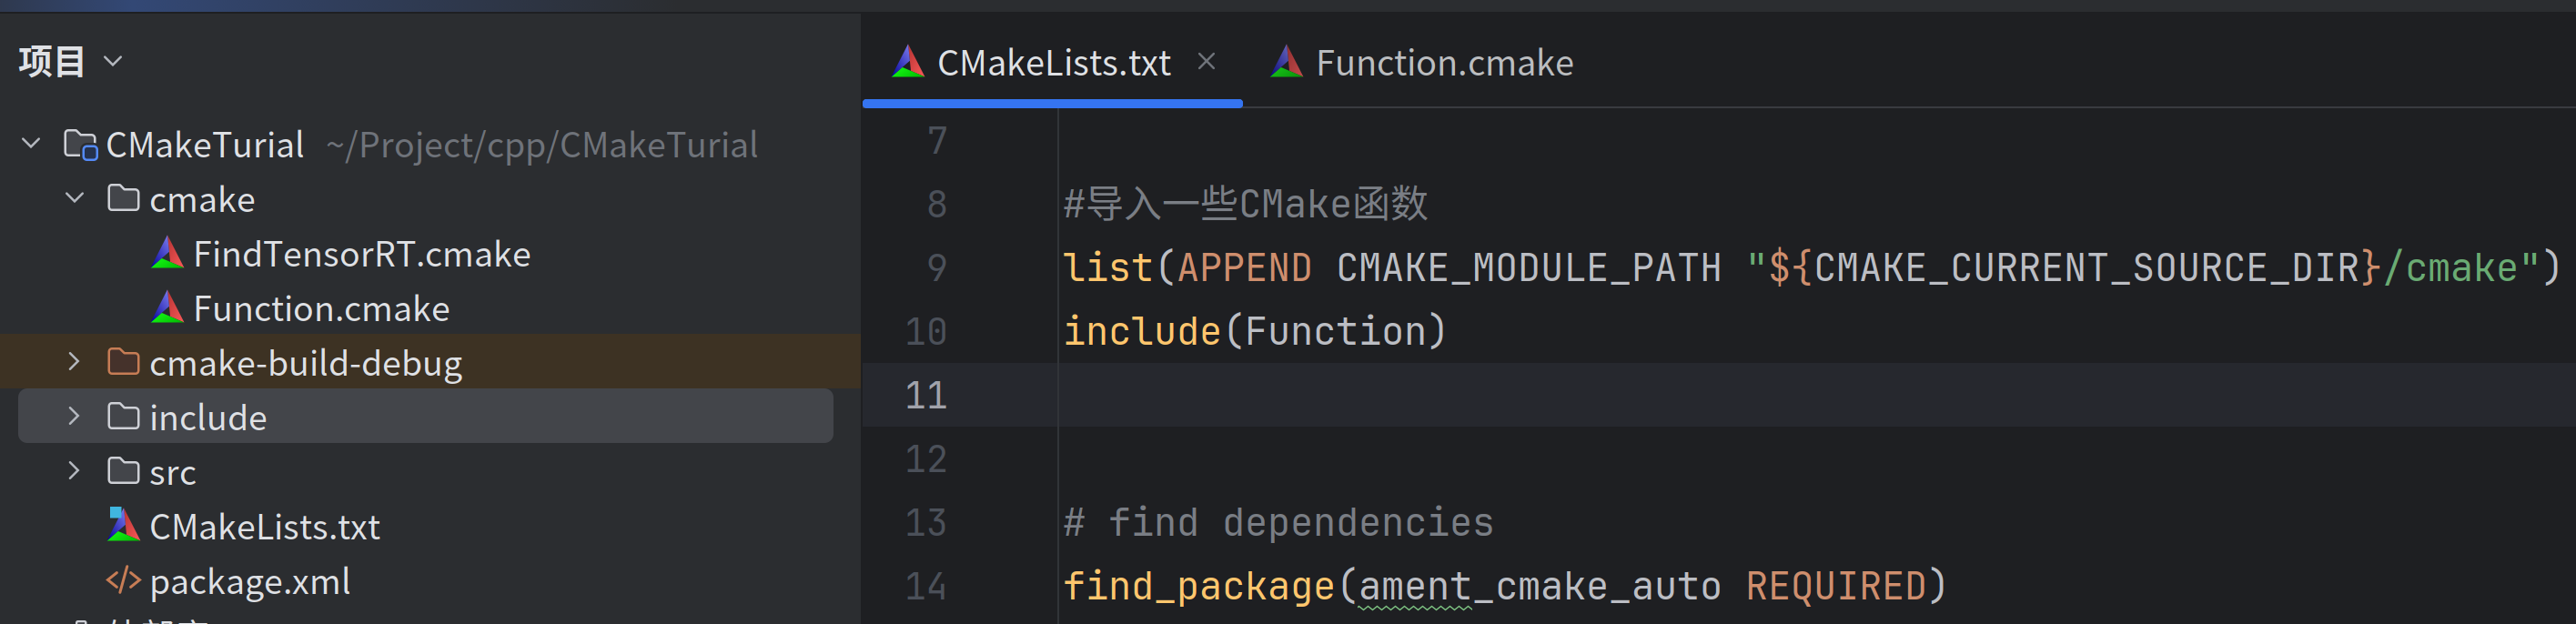
\includegraphics[width=0.7\textwidth]{cmake函数.png}
    \caption{实例项目结构} % 图片标题
    \label{fig:cmakeFunction} % 图片标签,用于引用
\end{figure}

这样,就可以在编译时打印出相关信息,方便调试。

\subsubsection{实例}

下面是一个实例项目的$CMakeLists.txt$文件,请试着读懂它:

\begin{tpython}
cmake_minimum_required(VERSION 3.8)
project(filter)

if(CMAKE_COMPILER_IS_GNUCXX OR CMAKE_CXX_COMPILER_ID MATCHES "Clang")
    add_compile_options(-Wall -Wextra -Wpedantic)
endif()

#导入一些CMake函数
list(APPEND CMAKE_MODULE_PATH "${CMAKE_CURRENT_SOURCE_DIR}/cmake")
include(Function)


# find_package 的高级平替,后面会讲
find_package(ament_cmake_auto REQUIRED)
ament_auto_find_build_dependencies()

###################项目目录设置######################
set(KALMAN_INCLUDE_DIR ${PROJECT_SOURCE_DIR}/include/kalman)
set(KALMAN_SRC_DIR ${PROJECT_SOURCE_DIR}/src/kalman)
set(MLS_INCLUDE_DIR ${PROJECT_SOURCE_DIR}/include/mls)
set(MLS_SRC_DIR ${PROJECT_SOURCE_DIR}/src/mls)
set(LMS_INCLUDE_DIR ${PROJECT_SOURCE_DIR}/include/lms)
set(LMS_SRC_DIR ${PROJECT_SOURCE_DIR}/src/lms)
set(EXEC_INCLUDE_DIR ${PROJECT_SOURCE_DIR}/include/exec)
set(EXEC_SRC_DIR ${PROJECT_SOURCE_DIR}/src/exec)

file(GLOB_RECURSE EXEC_SRCS ${EXEC_SRC_DIR}/*.cpp)
file(GLOB_RECURSE KALMAN_SRCS ${KALMAN_SRC_DIR}/*.cpp)
file(GLOB_RECURSE MLS_SRCS ${MLS_SRC_DIR}/*.cpp)
file(GLOB_RECURSE LMS_SRCS ${LMS_SRC_DIR}/*.cpp)

list(APPEND ALL_INCLUDE
        ${KALMAN_INCLUDE_DIR} ${MLS_INCLUDE_DIR} ${EXEC_INCLUDE_DIR} ${LMS_INCLUDE_DIR}
        ${OpenCV_INCLUDE_DIRS} ${EIGEN3_INCLUDE_DIR})

print_var(ALL_INCLUDE)

print_var(EXEC_SRCS)
print_var(KALMAN_SRCS)
print_var(MLS_SRCS)
print_var(LMS_SRCS)

include_directories(${ALL_INCLUDE})

##############静态库编译##################
add_library(filter_kalman ${KALMAN_SRCS})
add_library(filter_mls ${MLS_SRCS})
add_library(filter_lms ${LMS_SRCS})
list(APPEND FILTER_LIBS
        ${filter_kalman} ${filter_mls} ${filter_lms}
)
print_var(FILTER_LIBS)
############项目编译构建##########################
# add_executable的高级平替,以后会讲
ament_auto_add_executable(filter ${EXEC_SRCS})

target_link_libraries(filter ${OpenCV_LIBS} ${FILTER_LIBS})

# 这里进行项目的安装
if(BUILD_TESTING)
    find_package(ament_lint_auto REQUIRED)
    # the following line skips the linter which checks for copyrights
    # comment the line when a copyright and license is added to all source files
    set(ament_cmake_copyright_FOUND TRUE)
    # the following line skips cpplint (only works in a git repo)
    # comment the line when this package is in a git repo and when
    # a copyright and license is added to all source files
    set(ament_cmake_cpplint_FOUND TRUE)
    ament_lint_auto_find_test_dependencies()
endif()

# 神秘小代码,以后会讲
ament_auto_package()    
\end{tpython}

学了上面的内容,相信你已经可以写出自己的$CMakeLists.txt$文件了。


\section{ROS2基础}
在机器人开发过程中,我们往往需要使用到大量的传感器和执行机构,这时候,设备的有效管理和设备之间的通信就显得尤为重要,ROS2就是为了解决这一问题而生的。ROS2是一个开源的机器人操作系统,它提供了一系列的功能,包括:
\subsection{\textbf{引言:我们是如何从代码到机器人控制的}}
通过之前的学习,相信大家已经对如何再CMake的帮助下使用C++编写代码有了一定的了解。
之后你们会学习一些针对特殊需求的库,比如OpenCV、cuda等。他们能解决一些特定的问题,比如视觉处理
和模型运行等。

在此之前,你们需要学会如何把将要学的这些内容连接起来。比如,机器人的相机、传感器、MCU发来的信息会不断地
想你发送信息,我们需要一种“系统”能够从容地处理这些信息,对这些信息进行运算再发送出去。
这个“系统”其实就是操作系统(OS, Operating System)。对于个人计算机,我们使用的是Windows、Linux、Mac OS等,
他们帮我们进行了很多底层的工作,比如处理硬件、网络、驱动程序等。
而对于机器人来说,我们使用的是\textbf{ROS}(Robot Operating System),它帮助我们管理多个信息来源和不同信息,同时负责不同模块之间的通信。
这样一来,我们就不必要关注多个线程之间的同步、死锁等问题,只需要专注于业务逻辑的实现。
可以理解为如果不使用ROS2,我们需要自己使用C++的多线程库编写一个复杂的多线程系统,而ROS2可以替代你们上一章学的C++多线程,因为一个复多线程系统的编写
往往setTimeOut、wait等操作非常复杂,而ROS2使用DDS(Data Distribution Service)来实现通信,它已经帮我们处理了很多底层的细节。
\subsubsection{ROS2的版本}
和Linux与Ubuntu的关系类似,ROS2也有不同的版本或者说分支,比如ROS2 Foxy、ROS2 Eloquent等。
现在,我们队伍中主流使用的版本是\textbf{ROS2 Humble Hawksbill}。
\begin{figure}
    \centering
    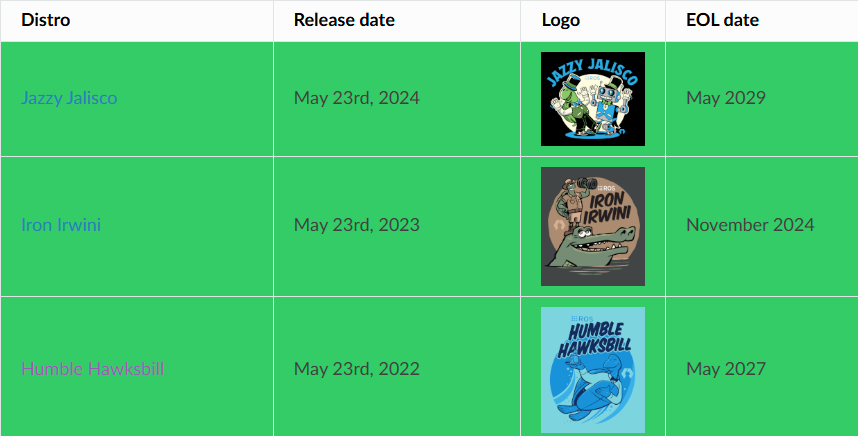
\includegraphics[width=0.8\textwidth]{Chapter4/img/ros2_logo.png}
    \caption{ROS2的最新版本跟新情况}
    \label{fig:ros2_logo}
\end{figure}

\subsubsection{ROS2的安装}

首先,我们需要安装ROS2的Humble Hawksbill 版本。
\begin{tbash}
    wget http://fishros.com/install -O fishros && . fishros
\end{tbash}
这条命令会帮你下载并运行一个脚本,根据它的引导选择下载ROS humble即可。
大概的输出为:
\begin{tbash}
    some output should be here...
\end{tbash}
这是一个非常好用的网站,江湖人称鱼香ROS。

这个命令在配置一个白板的Ubuntu系统时一般第一个运行,它会引导你更换系统源、安装必要的依赖包、配置环境变量等(甚至是下载QQ和微信)
这就减少了去官网上一个个寻找ubuntu版本的麻烦。

\subsection{ROS2架构}
\subsubsection{ROS2的系统架构}
ROS2的系统架构如下图所示:
\begin{figure}[h]
    \centering
    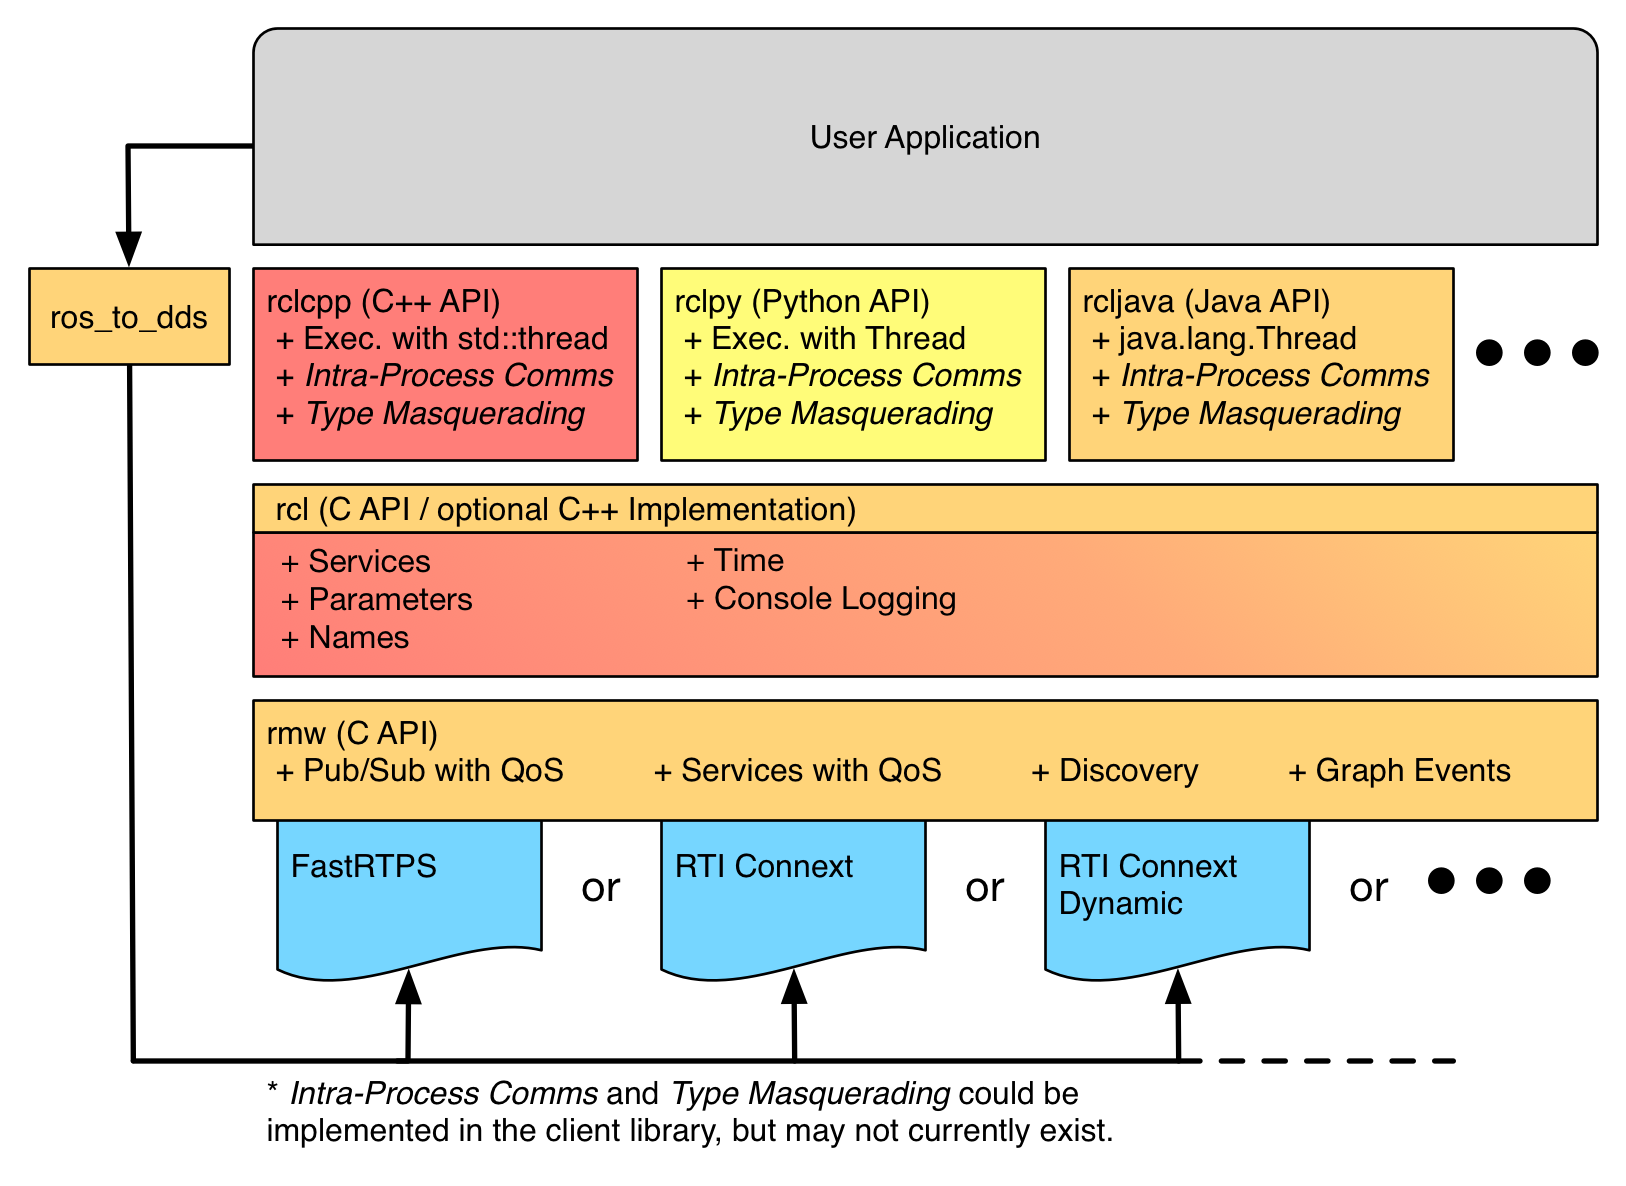
\includegraphics[width=0.8\textwidth]{Chapter4/img/ros2_arch.png}
    \caption{ROS2架构}
    \label{fig:ros2_arch}
    虽然你可能现在看不懂这个图,但不妨等学完之后再回过头来看看。
\end{figure}
一些需要听说过的属于的翻译:
\begin{itemize}
    \item \textbf{rclcpp}: ROS Client Library for C++,它是ROS2的C++客户端库,负责ROS2节点的创建、通信、生命周期管理等,我们使用的主要是这个库。
    \item \textbf{rmw}: ROS Middleware,它是ROS2的中间件,负责底层通信的实现。
    \item \textbf{Qos}: Quality of Service,它是ROS2的通信质量保证机制,用来控制通信的延迟、带宽等。
    \item \textbf{DDS}: Data Distribution Service,它是ROS2的分布式数据服务,用来实现ROS2节点之间的通信。
\end{itemize}
\subsubsection{ROS2的节点与组件}
\textbf{ROS2的基本思想是分布式的、模块化的。}

ROS2的节点是ROS2系统的基本单元,它可以包含多个ROS2组件。

我们可以用这个图来直观地理解ROS2的\textbf{节点}:
\begin{figure}[h]
    \centering
    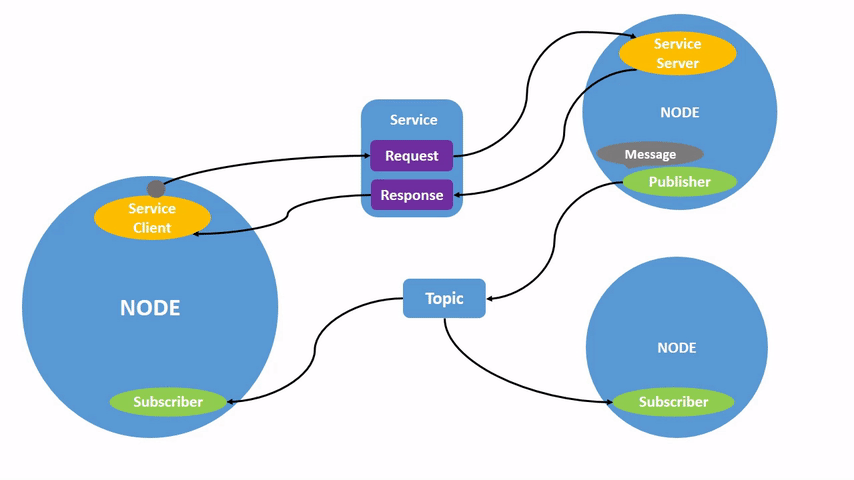
\includegraphics[width=0.8\textwidth]{Chapter4/img/ros2_node.png}
    \caption{ROS2节点与组件}
    \label{fig:ros2_node}
\end{figure}
这是一个动图,你可以去\underline{\href{https://docs.ros.org/en/humble/_images/Nodes-TopicandService.gif}{这里}}播放看看。

这个图直观的反映了ROS2的模块化是依靠\textbf{节点}完成的,节点的职责可以是接收某个传感器的信息(比如相机),也可以是对数据进行处理的流程(比如对相机的图像进行滤波),也可以是提供服务(比如反馈相机的参数信息)
当然这些功能也可以在一个节点中完成。同时可以注意到,节点之间的信息交流是依靠组件(Component)来实现的,一般来说一个节点的运行入口函数也是某个组件的回调函数。


对于我们实际上手操作的情况下,我们更感知的操作方式有两种。
一是使用CLI tools(command-line interface),二是使用Client Libraries。
我们一般使用CLI tools来创建、运行、调试节点,而Client Libraries则用于编写节点的逻辑。

\subsection{ROS2的节点}
ROS2的节点是ROS2系统的基本单元,它可以包含多个ROS2组件,比如发布者(Publisher)、订阅者(Subscriber)、服务(Service)、客户端(Client)等。
下面我们先从什么是节点开始介绍。

\subsection{ROS2}

https://design.ros2.org/articles/roslaunch.html

\section{OpenCV与图像处理基础}
在计算机处理过程中,图像处理是一种重要的任务。OpenCV是开源的计算机视觉库,它提供了一系列的图像处理算法,包括图像的读取、写入、显示、裁剪、缩放、旋转、滤波、轮廓检测、特征提取、匹配、形态学处理等。

\section{神经网络与深度学习基础}
机器学习是人工智能领域的一个重要研究方向,它利用大量的数据训练模型,从而对未知的输入进行预测。深度学习是机器学习的一个分支,它利用神经网络来学习复杂的非线性函数。

\subsection{了解神经网络}
如今神经网络在各个领域都有涉及, 在计算机视觉领域更是有极大的优越性。从机器学习再到深度学习,几乎已经形成一个完整的
技术体系并且仍然在高速发展。
通常来说,神经网络一般有以下三个作用:
\begin{enumerate}
    \item \textbf{预测}: 这通常是一维层面的,通过给予计算机一定量已有的数据(通常是多组自变量和因变量)拟合出一个合适的曲线(函数),当有新的自变量传入的时候,通过该曲线给出预测的结果
    \item \textbf{识别}: 这通常是二维层面的,同样是给予计算机一定量的二维图像,同时告诉计算机我们想要识别的图像主体,给予其标注,通过大量数据的学习让计算机能够准确识别任意图像中符合要求的部分
    \item \textbf{自然语言}: 通过给予海量的文本数据,使计算机能够理解、解释和生成自然语言,进行情感分析和语言推断。
\end{enumerate}
这些只是对作用的简单解释,具体过程要比这复杂的多。

无论是一维的预测还是二维的识别,从本质上来说,所谓\textbf{学习},就是不断调整神经网络内部参数使参数达到一种足够泛化也足够准确的大小,能够保证传入
的数据在经过这群参数组成的\textbf{“函数"}映射后,得到一个可信度高的答案。
那么在拟合这群参数后,如果没有处理好,会出现\textbf{欠拟合}和\textbf{过拟合}的问题

\begin{figure}[h]
    \centering
    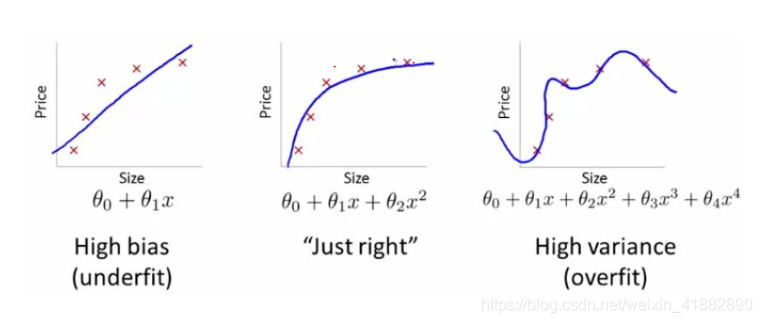
\includegraphics[width=0.8\textwidth]{拟合.png}
    \caption{欠拟合与过拟合}
    \label{fig:拟合}
\end{figure}

如图所示,欠拟合就是参数调整的太差了,根本没有预测的能力,得到的答案和实际上差距非常大,这时候我们就应该考虑增加训练数据或者
是增强数据的特征。

另一个过拟合,就是数据的特征过于明显或者是训练的过强导致网络没有足够的泛化能力,那么当传入的数据不是训练的数据的时候,将无法正确
预测,这时候就应该减少训练的次数,减少数据集的数量或者是降低数据的特征,提高泛化能力,

通过简单的了解,我们知道神经网络的作用以及神经网络是如何训练出来的,现在我们将通过自己动手搭建一个神经网络,在学习搭建的过程中对
更深入的内容进行讲述。
\subsection{动手搭建神经网络}
如果我们的网络只有简单的功能需求,那么用当今主流的pytorch就可以快速构建起一个神经网络,pytorch中封装好了很多搭建网络所需要的功能
我们只需要简单理解就能够直接调用使用。如果我们对准确性,效率等有更高的要求,可以使用已有的框架比如yolo,只需要准备好数据集和标注,按照需求
简单调整一下框架的参数,就可以训练出一个高性能的网络。

我们将从安装开始,一步步利用\textbf{pytorch}搭建出一个简单的识别图像中数字的网络。
\subsubsection{虚拟环境——Anaconda}
在安装Pytorch之前,我们要先安装Anaconda。

什么是Anaconda?一般来说在电脑上已经安装好了一个python环境,但是对于不同的项目需要不同的python环境
同时这些项目还要安装各种包和依赖,如果都把他们放在我们电脑最基础的环境下,很容易出现各种冲突问题而且很难管理。Anaconda能为我们创建不同的虚拟环境,
我们可以按照需要在这些虚拟环境里安装不同的包和依赖,它们不会相互影响,而且不同环境之间相互切换,操作简单,非常方便。同时Anaconda还有超过180个科学包和
依赖项,简单的几行命令就可以将这些包安装到指定的虚拟环境下,省去了麻烦的下载流程和令人头疼的配置过程。我们将用Anaconda创建一个独属于pytorch的虚拟环境。

Anaconda官方下载地址:\url{https://www.anaconda.com/download/}

按照官方流程安装好Anaconda后,在Windows的Anaconda Prompt(ubuntu的终端)输入
\begin{tbash}
    conda --version
\end{tbash}
如果显示版本号,说明安装成功。

\textbf{创建虚拟环境}

在Anaconda Prompt输入
\begin{tbash}
    conda create -n pytorch python=3.7
\end{tbash}
这样我们就创建了一个名为pytorch的虚拟环境,同时指定了python的版本为3.7,这样我们就可以在这个环境下安装pytorch了。

\textbf{激活虚拟环境}

在Anaconda Prompt输入
\begin{tbash}
    conda activate pytorch
\end{tbash}
我们会发现命令行前面多了(pytorch)字样,这就说明我们已经成功激活了pytorch环境。
这时输入
\begin{tbash}
    pip list
\end{tbash}
就可以看到当前环境下已经安装的包。
类似的
\begin{tbash}
    conda deactivate
\end{tbash}
就退出了当前环境。

\subsubsection{安装Pytorch}
在激活了pytorch环境后,我们就可以安装pytorch了。
在命令行输入
\begin{tbash}
    pip install pytorch torchvision
\end{tbash}
这样我们就安装好了pytorch,同时还安装了torchvision这个包是pytorch的辅助包,用于处理图像。
\textit{如果你出现了诸如网络问题导致无法安装,请改变虚拟环境的源为国内源,具体操作请自行搜索}

这样我们就安装好了pytorch-CPU,如果你有NVIDIA的显卡,可以考虑安装pytorch-GPU,网络的训练速度和推理速度会更快。
可以在命令行输入
\begin{tbash}
    nvidia-smi
\end{tbash}
查看自己的显卡型号,然后在官网上查看对应的CUDA版本,再安装对应的pytorch-GPU版本。
这里给上CUDA的官网下载地址:\url{https://developer.nvidia.com/cuda-toolkit-archive}
刚刚的pip install命令可以改为
\begin{tbash}
    pip3 install torch torchvision torchaudio --index-url https://download.pytorch.org/whl/cu{你的CUDA版本}
\end{tbash}

\subsubsection{搭建神经网络}
接下来用pytorch搭建一个简单的LeNet网络,识别MNIST数据集中的手写数字

选择一个你喜欢的IDE,比如VSCode, Pycharm, Clion等,创建一个python文件,选择解释器为刚刚创建的虚拟环境。
如果你感觉IDE的配置比较麻烦,也可以试试jupyter notebook,它是一个交互式的笔记本,可以直接在浏览器上运行代码,适合学习使用。

准备好后,首先导入需要的包
\begin{tpython}
    import torch
    import torch.nn as nn
    import torch.optim as optim
    import torchvision
    import torchvision.transforms as transforms
    import matplotlib.pyplot as plt
\end{tpython}
\begin{enumerate}
    \item torch: pytorch的核心包,包含pytorch的核心数据结构,以及所有的操作
    \item torch.nn: pytorch的神经网络包,包含所需的神经网络模块。
    \item torch.optim: pytorch的优化器包,包含了所有的优化器。
    \item torchvision: pytorch的图像处理包,包含了图像处理的所有操作。
    \item torchvision.transforms: pytorch的图像变换包,包含了所有的图像变换操作。
    \item matplotlib.pyplot: 画图的包,我们用来画出训练过程中的一些曲线。
\end{enumerate}

接下来准备MINST数据集

MINST数据集是一个包含了6万张训练图片和1万张测试图片的数据集,每张图片都是各式各样的手写的数组,每张图片上都有一个0-9的数字标签。
我们可以通过torchvision包中的datasets来下载这个数据集。
\begin{tpython}
    train_dataset = torchvision.datasets.MNIST(root='./data', train=True, transform=transforms.ToTensor(), download=True)
    test_dataset = torchvision.datasets.MNIST(root='./data', train=False, transform=transforms.ToTensor(), download=True)
\end{tpython}
这里的参数含义分别是:
\begin{enumerate}
    \item root: 数据集的存放路径
    \item train: 是否是训练集,True表示训练集,False表示测试集
    \item transform: 数据集的变换方式,这里是ToTensor(),将图片转换为tensor张量
    \item download: 是否下载数据集,如果已经下载过了,可以设为False
\end{enumerate}

但这里我们需要对数据集进行更多的转变操作,利用Compose将多个变换组合在一起,比如ToTensor()转化成Tensor和Normalize归一化
\begin{tpython}
    compose=torchvision.transforms.Compose([
        torchvision.transforms.ToTensor(),
        torchvision.transforms.Normalize((0.1307,), (0.3081,))
    ])

    train_dataset = torchvision.datasets.MNIST(root='./data', train=True, transform=compose, download=True)
    test_dataset = torchvision.datasets.MNIST(root='./data', train=False, transform=compose, download=True)
\end{tpython}

然后通过DataLoader加载数据集,使我们可以迭代访问数据集
\begin{tpython}
    train_loader = torch.utils.data.DataLoader(dataset=train_dataset, batch_size=64, shuffle=True)
    test_loader = torch.utils.data.DataLoader(dataset=test_dataset, batch_size=64, shuffle=False)
\end{tpython}
这里的参数含义分别是:
\begin{enumerate}
    \item dataset: 加载的数据集
    \item batch\_size: 一次加载的数据量, 这里是$64$
    \item shuffle: 是否打乱数据集
\end{enumerate}

我们完成了对数据集的准备,接下来搭建最基础最经典的LeNet网络结构:
\begin{figure}[H]
    \centering
    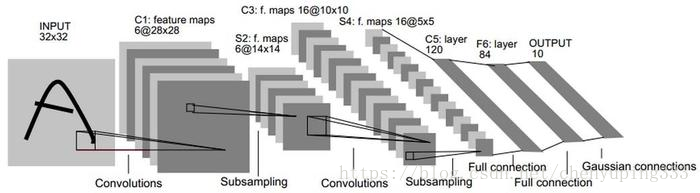
\includegraphics[width=0.7\textwidth]{images/LeNet.png}
    \caption{LeNet网络结构}
    \label{fig:LeNet}
\end{figure}

可以看到,除去输入层,LeNet一共有7层,按顺序进行卷积,池化,卷积,池化,全连接,全连接,全连接操作。

我们先对卷积,池化操作进行解释。

\textbf{卷积操作}:

卷积操作是神经网络中基本也是重要的操作之一,目的是提取图像的特征,通过一个n*n的卷积核在图像上滑动,将卷积核中心的像素大小替换为该卷积核上所有像素大小的加权和
\begin{figure}[H]
    \centering
    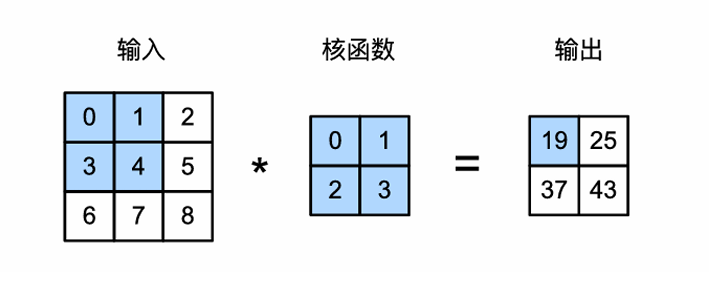
\includegraphics[width=0.7\textwidth]{images/卷积.png}
    \caption{卷积操作}
    \label{fig:卷积}
\end{figure}
用公式表示为:
\begin{equation}
    [H]_{i,j}=\sum_{a=-\Delta }^{\Delta}\sum_{b=-\Delta}^{\Delta}[V]_{a,b}[X]{i+a,j+b}   
\end{equation}
其中$[H]$是卷积后的图像,$[V]$是卷积核,$[X]$是原图像,$\Delta$是卷积核的大小。
这就是一次卷积层的操作。

我们要根据需要调整卷积核的大小,填充,步幅等参数。
\begin{enumerate}
    \item 卷积核大小: 通常是一个奇数,比如$3\times3$,$5\times5$,$7\times7$等
    \item 填充: 由于卷积核不是$1\times1$,所以边缘像素无法进行卷积,在多次卷积后,图像像素显著减少会失去许多信息,这就需要填充对图像进行扩充。
    \item 步幅: 卷积核每次滑动的步长,步长越大,卷积出的图像尺寸越小
\end{enumerate}
一般输出图像的形状为
\begin{equation}
    (n_{h}-k_{h}+p{h}+1) \times (n_{w}-k_{w}+p_{w}+1)
\end{equation}
其中$n_{h},n_{w}$是输入图像的高和宽,$k_{h},k_{w}$是卷积核的高和宽,$p_{h},p_{w}$是填充的高和宽。

\textbf{池化操作}:

池化操作是为了减少数据量,减少计算量,同时保留图像的主要特征,目的是减低卷积层对位置的敏感性。

汇聚层和卷积层相似,由一个池化核(池化窗口)在输入的信息上移动,同
样具有填充和步幅两个参数。汇聚操作计算的是窗口
中数据的最大值或者是平均值,这些操作分别称为\textbf{最大汇聚层}和\textbf{平均汇聚层}
\begin{figure}[H]
    \centering
    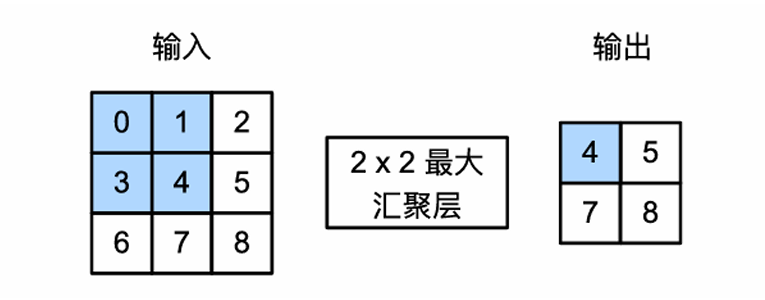
\includegraphics[width=0.7\textwidth]{images/池化.png}
    \caption{池化操作}
    \label{fig:池化}
\end{figure}

\textbf{全连接层}:

全连接层通常作为输出层使用,负责将网络的高层特征映射到最终的类别概率。
通常是为了整合特征,减少特征的维度,得到最终的输出类别。

\textbf{激活函数}:

这里我们涉及一下激活函数。
激活函数是神经网络中非常重要的一部分,它的作用是引入非线性因素,使得神经网络可以拟合任意复杂的函数。
通过加权和以及偏置来确定神经元是否应该激活,将输入信号转换为输出的
可微运算。大多数激活函数都是非线性的。
我们将主要用到ReLU激活函数,这是一个非常纯粹的函数:
\begin{equation}
    ReLU(x)=max(0,x)
\end{equation}
抛弃所有负元素,它求导表现得特别好:要么让参数消失,要么让参数通过

除此之外,还有sigmoid函数:
\begin{equation}
    sigmoid(x)=\frac{1}{1+\exp{-x}} 
\end{equation}
又称挤压函数,将($-\infty$,$\infty$)的任意数压缩到( $0$ , $1$ )

如此我们了解了神经网络的一些基本操作。

\textbf{搭建网络}:

首先写一个LeNet类,继承nn.Module
\begin{tpython}
    class LeNet(nn.Module):
        def __init__(self):
            super(LeNet, self).__init__()
            self.conv1=nn.Conv2d(1,6,5)
            self.pool1=nn.MaxPool2d(2,2)
            self.conv2=nn.Conv2d(6,16,5)
            self.pool2=nn.MaxPool2d(2,2)
            self.fc1=nn.Linear(16*5*5,120)
            self.fc2=nn.Linear(120,84)
            self.fc3=nn.Linear(84,10)
\end{tpython}

我们这里定义了LeNet类,并且在初始化函数中定义了一些层
显而易见
\textbf{卷积层}:
\begin{tpython}
    self.conv1=nn.Conv2d(3,16,5)
\end{tpython}
参数分别是\textbf{输入通道数,输出通道数,卷积核大小}。
我们知道图片是由RGB三个通道组成,因此这里输入通道数为3,按照LeNet的结构,让输出通道数为16,这是第一个卷积层。第二个卷积层同理,输入通道数为16,输出通道数为32。

\textbf{池化层}:
\begin{tpython}
    self.pool1=nn.MaxPool2d(2,2)
\end{tpython}
参数分别是\textbf{池化核大小,步幅}。
这里的池化核大小是2,步幅也是2,这是第一个池化层。第二个池化层同理。

\textbf{全连接层}:
\begin{tpython}
    self.fc1=nn.Linear(16*5*5,120)
\end{tpython}
参数分别是\textbf{输入特征数,输出特征数}。
输入特征数数根据上一层也就是池化层的输出决定。后面两个全连接层同理。
在最后一个全连接层我们输出10个特征,因为MNIST数据集中有10个类别(0 ~ 9)。

接下来我们定义前向传播函数,也就是网络的计算过程,处理输入数据,输出预测结果。
\begin{tpython}
    def forward(self, x):
        x=nn.relu(self.conv1(x))
        x=self.pool1(x)
        x=nn.relu(self.conv2(x))
        x=self.pool2(x)
        x=x.view(-1,16*5*5)
        x=nn.relu(self.fc1(x))
        x=nn.relu(self.fc2(x))
        x=self.fc3(x)
        return x
\end{tpython}
和上面的架构一样,只是在每次卷积操作后进行了激活操作,以及全连接层后进行了激活操作。
\textbf{x.view}:
这个函数是将一个多维的tensor转换为一维的tensor,参数-1表示自动计算,这里是将16*5*5的tensor转换为一维的tensor。
符合后面的全连接层输入。

如果想让网络每个处理更加简洁,可以使用\text{Sequential容器},将网络的层组合在一起。
比如我们可以将一次卷积,激活,池化操作组合在一起
\begin{tpython}
    self.conv1=nn.Sequential(
        nn.Conv2d(3,16,5),
        nn.ReLU(),
        nn.MaxPool2d(2,2)
    )
\end{tpython}
这样在forward函数中就可以直接调用这个容器,更加简洁。

这样我们就搭建好了一个简单的LeNet网络
\begin{tpython}
    Net=LeNet() 
\end{tpython}
实例化我们的网络

\textbf{定义损失函数:}

损失函数负责责量化实际值和预测值之间的差距,数值越小损失越小,因此我们通常要追求更小的损失。比如,平方误差函数
\begin{equation}
    l^{(i)}(\textbf{w},b)=\frac{1}{2}(\hat{y}^{(i)}-y^{(i)})^{2}
\end{equation}
$\hat{y}$表示预测值,$y$表示实际值,公式代表在$w$权重,$b$偏置下预测值和实际值的误差
一般情况下,我们要计算训练集上n个样本的平均损失L
\begin{equation}
    L(\textbf{w},b)=\frac{1}{n}\sum_{i=1}^{n}l^{(i)}(\textbf{w},b)
\end{equation}

在LeNet中我们使用\textbf{交叉熵损失函数}:
交叉熵公式:
\begin{equation}
    H(y,\hat{y})=-\sum_{i}y_{i}\log{\hat{y}_{i}}
\end{equation}
其中y是实际值,$\hat{y}$是预测值,交叉熵损失函数是一个非负函数,当预测值和实际值相等时,交叉熵为0,否则交叉熵越大,预测值和实际值差距越大。

代码中我们定义损失函数:
\begin{tpython}
    criterion=nn.CrossEntropyLoss()
\end{tpython}

\textbf{定义优化器:}

优化器负责更新网络的参数,使得损失函数最小化,这里我们使用\textbf{Adam优化器}:
Adam优化器是一种自适应学习率的优化器,它可以根据梯度的大小自动调整学习率,使得训练更加稳定。
所谓\textbf{学习率},就是每次更新参数的步长,学习率越大,参数更新的幅度越大,学习率越小,参数更新的幅度越小。
因此动态调整学习率有一定的重要性,降低梯度爆炸和梯度消失的风险。

\begin{tpython}
    optimizer=optim.Adam(Net.parameters(),lr=0.001)
\end{tpython}
这里的参数含义分别是\textbf{网络的参数,学习率}。Net.parameters()自带的函数,可以返回网络中所有的参数。

我们已经定义好了网络,损失函数,优化器,接下来我们就可以开始训练网络了。

\subsubsection{训练与测试网络}
在定义训练函数之前,我们需要了解一下网络训练过程中调整参数的主要方式——\textbf{反向传播}:

首先是\textbf{前向传播},前向传播是指从输入层到输出层的计算过程,通过输入数据,经过一系列的计算,得到输出结果。
这期间会储存一些中间变量,以便后续的反向传播。

反向传播是计算神经网络参数梯度的方法,该方法根据微积分中的\textbf{链式规则},按相反的
顺序从输出层到输入层遍历网络。该算法存储了计算某些参数梯度时所需的任何中间变量(偏导数)

在训练神经网络时,在初始化模型参数后,我们交替使用前向传播和反向传播,利用反向传播给出的梯度来更新模型参数。

\textit{反向传播需要利用前向传播中储存的中间值,因此我们一般需要保存这些中间值,这就导致需要更大的显存。
这些中间值的大小与网络层的数量和批量的大小大致成正比。
因此,使用更大的批量来训练更深层次的网络更容易导致\textbf{显存}不足(out of memory)错误}

就像前面所说的,神经网络训练本质上是调整参数,参数好坏的标准就是损失函数,我们要让损失函数尽可能的小,这其中用到了一个非常重要的算法——\textbf{梯度下降}:
梯度下降是一种优化算法,通过不断的往损失函数减小的方向上来更新参数以此降低误差,来达到优化模型的目的。
更新过程:
\begin{equation}
    (\textbf{w},b) \longleftarrow (\textbf{w},b) - \frac{\eta}{\left\lvert\mathcal{B}\right\rvert}\sum_{i\in\mathcal{B}}\partial_(\textbf{w},b)l^{(i)}(\textbf{w},b)
\end{equation}
\begin{enumerate}
    \item $\eta$: 学习率,控制参数更新的步长
    \item $\mathcal{B}$ : 批量大小,每次更新参数的样本数
    \item $\partial$ : 偏导数,迭代的是哪个参数就对哪个参数求偏导
    \item $l^{(i)}$ : 损失函数求得的损失
\end{enumerate}
这其中\textbf{学习率和批量}是手动设置的,是\textbf{超参数}。需要不断调整来达到最优效果。
在实际过程中,超参数的设置是十分关键的,这需要常年累月的调参经验。

\textit{算法只能使损失向最小值缓慢\textbf{收敛},无法在有限步数下准确求出最小值}

接下来我们定义train函数,用于训练网络
\begin{tpython}
    def train(epoch) # 传入当前的轮次
        running_loss=0.0 # 累加损失
        running_total=0 # 累加样本总数
        running_correct=0 # 累加正确样本数
        for batch_idx, data in enumerate(train_loader,0): # 遍历训练集
            inputs, labels=data # 获取输入和标签
            optimizer.zero_grad() # 梯度清零

            # forward + backward + optimize
            outputs=Net(inputs) # 前向传播
            loss=criterion(outputs,labels) # 计算损失
            loss.backward() # 反向传播
            optimizer.step() # 更新参数,优化

            running_loss+=loss.item() # 累加损失
            _, predicted=torch.max(outputs,dim=1) # 获取预测值
            running_total+=inputs.shape[0] # 累加样本总数
            running_correct+=(predicted==labels).sum().item() # 累加正确样本数

            if batch_idx % 300 == 299: # 不想要每一次都出loss, 选择每300次出一个平均损失, 和准确率
                print('[%d, %5d]: loss: %.3f , acc: %.2f %%'
                % (epoch + 1, batch_idx + 1, running_loss / 300, 100 * running_correct / running_total))
                running_loss = 0.0
                running_total = 0
                running_correct = 0
\end{tpython}

其中累加损失,累加样本总数,累加正确样本数是为了计算平均损失和准确率,这样我们可以更直观的看到网络的训练情况。
利用\textbf{enumerate}函数将train\_loader转换为一个迭代器,每次迭代返回一个batch的数据,同时返回一个索引,这样我们就可以知道当前是第几个batch。
\textbf{optimizer.zero\_grad()}是将梯度清零,因为pytorch默认会将梯度累加,所以每次迭代前都要清零。
然后经过前向传播获取到输出,将输出和标签传入损失函数,计算输出和标签之间的差距,也就是损失。
通过得到的损失,进行反向传播,更新网络中的参数,用优化器优化网络。

这样就完整的定义了一个训练函数,你也可以通过:
\begin{tpython}
    torch.save(model, f"../save/model_{epoch+1}.pth")
\end{tpython}
在指定路径下保存模型,以便后续使用。

\textbf{测试函数}:

训练完网络后,我们需要测试网络的性能,测试函数和训练函数类似,只是不需要反向传播和更新参数。
\begin{tpython}
    def test(epoch):
        correct=0 # 正确样本数
        total=0 # 总样本数
        with torch.no_grad(): # 测试集不需要算梯度
            for data in test_loader:
                images, labels=data # 获取输入和标签
                ouputs=Net(images)
                _, predicted=torch.max(outputs,dim=1)
                total+=labels.size(0)
                correct+=(predicted==labels).sum().item()
        acc=correct/total
        print('[%d / %d]: Accuracy on test set: %.1f %% ' % (epoch + 1, EPOCH, 100 * acc))  # 求测试的准确率,正确数/总数
\end{tpython}
测试函数和训练函数类似,只是获取在不需要梯度的情况下进行的。
correct和total是用来计算正确率的,方便我们看到网络的性能。

这样就定义了一个测试函数,接下来只需要在主函数中调用这两个函数,就可以训练和测试网络了。
\begin{tpython}
    if __name__ == '__main__':
        for epoch in range(50):
            train(epoch)
            test(epoch)
\end{tpython}

到此,成功完成了LeNet网络的训练和测试。这并不是一个很复杂的网络,但是确实包含了当今主流网络的主要操作。
当今网络的发展已经非常成熟,有很多优秀的网络结构,比如VGG,ResNet,DenseNet等,这些网络结构都有自己的特点。
它们都是基于LeNet的基础上不断发展而来,通过不断的尝试和改进,才有了现在的网络结构。
如果你掌握了LeNet的基本操作,那么学习其他网络结构就会变得更加容易。

\subsubsection{模型的导出和使用}
我们利用torch.save()函数将模型保存下来后,可以在其他地方加载模型,继续训练或者是直接使用。

\textbf{模型的使用:}
\begin{tpython}
    model=torch.load('model.pth')
    model.eval() # 将模型设置为评估模式
    with torch.no_grad():
        output=model(input) # 得到输出
        print(output)
\end{tpython}

\textbf{\textit{*利用GPU加速训练:}}

如果你有NVIDIA显卡,并且按照上面的步骤安装了pytorch-GPU版本,只需要在代码中简单加几行代码,就可以实现在
GPU上训练我们的模型。由于显卡的特性,GPU运算过程中,需要指令和数据都存储在显存中。
对于我们的神经网络就是,将网络结构,损失函数和数据都加载到显存中,然后进行运算。
可以使用$.cuda()$函数将模型加载到GPU上,然后在训练过程中,将数据也加载到GPU上进行运算,
使用$.to('cpu')$将数据转移到内存中,便于后续的处理。
GPU相比于CPU牺牲了大部分在CPU上属于缓存区等区域的面积,用来放更多的运算核心,因此GPU比
CPU更适合并行运算,运算速度更快,更适合网络模型训练,去处理大量的数据。

比如在代码中,我们加上
\begin{tpython}
    # model声明后
    model.cuda()
    ....
    ....
    # train函数中
    inputs, labels=data
    inputs=inputs.cuda()
    labels=labels.cuda()
    ....
    ....
    # test函数中
    images, labels = data
    images = images.cuda()
    labels = labels.cuda()
    
    # 在损失函数下也可以加上
    loss_function = loss_function.cuda()
\end{tpython}
再次训练,你会发现训练速度大大提升,从loss的输出就可以看出。

\textbf{\textit{*关于YOLO等框架:}}

YOLO是一个非常优秀的目标检测框架,它的全称是You Only Look Once,它的特点是速度快,准确率高,适合实时目标检测。
YOLO如今仍然在不断迭代更新,如今已有诸如YOLO-v5,YOLO-v8,YOLO-v10等一系列的版本。
其支持不同功能模型的训练,比如detect(检测),classify(分类),pose(姿态估计)等。

\begin{figure}[H]
    \centering
    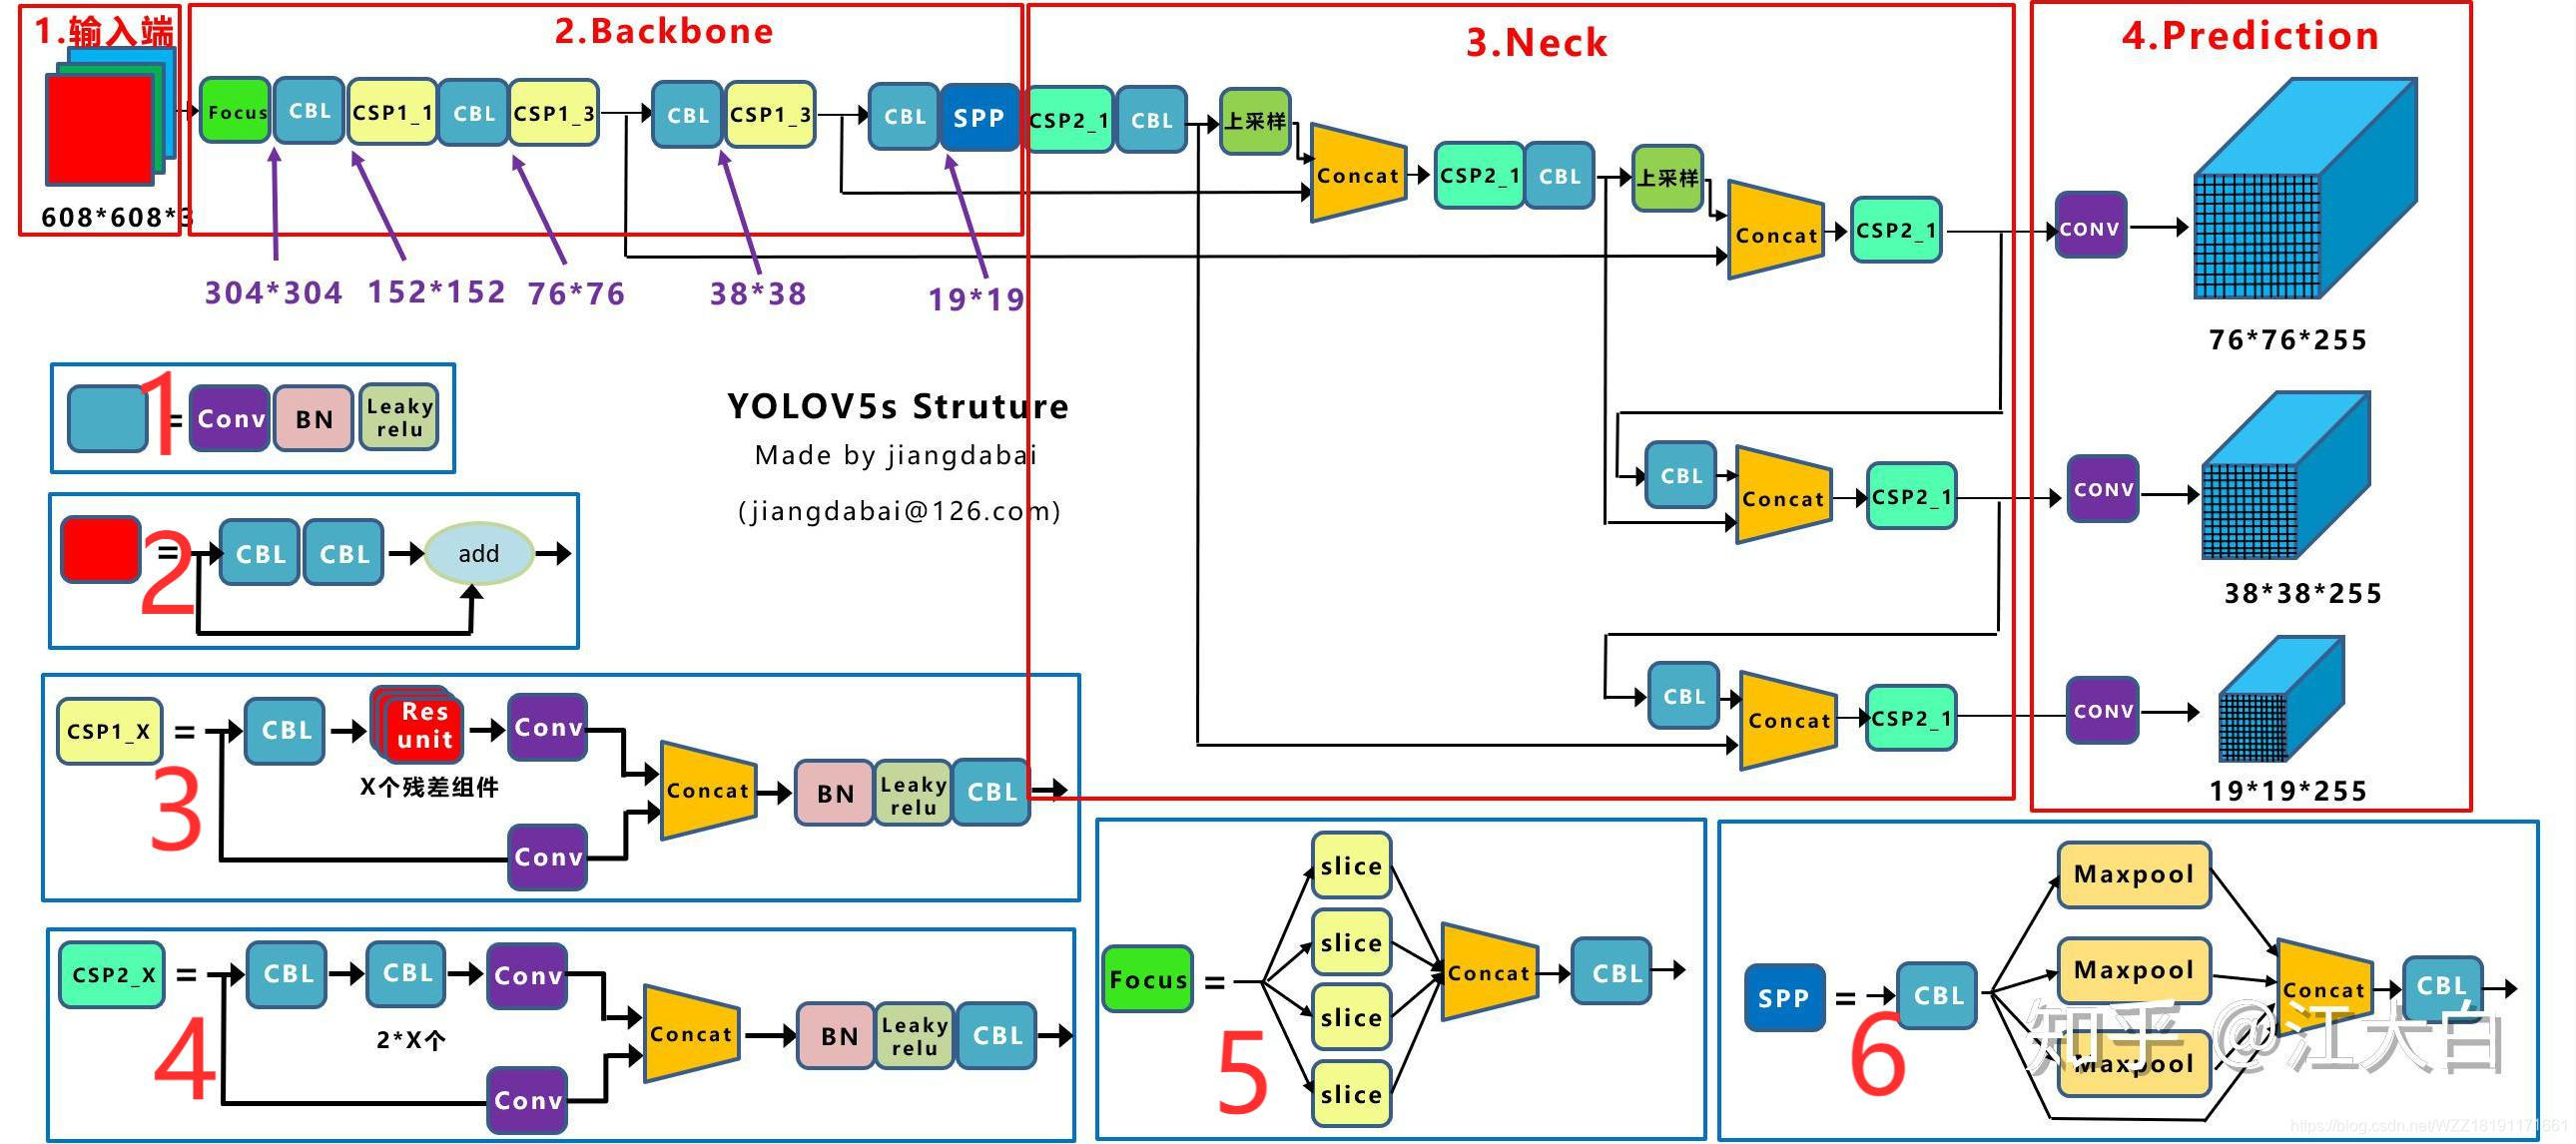
\includegraphics[width=0.8\textwidth]{images/YOLOv5.jpeg}
    \caption{YOLOv5网络架构}
    \label{fig:YOLOv5}
\end{figure}

可以通过这里了解:\url{https://github.com/THU-MIG/yolov10}

\url{https://blog.csdn.net/WZZ18191171661/article/details/113789486}

\subsection{简单了解模型部署}
如果我们已经拥有了一个训练好的模型,但是事实上这并不能草草的生搬硬套在我们实际的项目中。
一个项目通常不会是在拥有着高性能的NVIDIA显卡和高性能的CPU上运行的,通常是在一些性能较低的设备上,比如
在机器人上,代码运行在minipc,而minipc的性能和配置有限(intel旗下的nuc甚至没有GPU),因此我们需要尽量激发设备的性能,提高模型的推理速度。
这就要涉及到模型的部署。

\begin{enumerate}
    \item \textbf{CPU上的模型部署}: intel官方提供了一个完整的开源的部署工具——openvino,利用openvino提供的C++接口,可以将训练好的模型转换为openvino支持的模型,然后在CPU上运行,可以大大提高模型的推理速度。
    \item \textbf{GPU上的模型部署}: NVIDIA也提供了一个完整的开源的部署工具——tensorRT,同样也可以利用相应的API使得模型在GPU上实施推理,拥有更快的推理速度.
\end{enumerate}

\textbf{\textit{*有关模型文件类型:}}

模型文件的类型并不是单一的,不同的框架支持的是不同的文件类型。
譬如pytorch导出的模型为.pth文件,YOLO框架导出的是.pt文件。
而在openvino部署模型的时候,又需要把模型转换没xml和bin文件。
tensorrt所需的又是.engine文件。

模型文件类型的不同确实是一件麻烦的事情,因此领域内出现了一种.onnx文件,它使得不同的深度学习框架之间可以互操作。
openvino和tensorrt都支持对onnx文件的转换。有相应的API可以将onnx文件转换为自身所需要的文件类型。YOLO官方也给出了
相关的指令能够一键转换将.pt转换为.onnx文件。onnx文件就像是一个中间文件,使得不同框架之间的转换变得更加容易。

\textit{如果你有一个ONNX文件,你可以访问网站:\url{https://netron.app/}查看ONNX文件的结构,方便了解模型的结构}

\subsection{总结}
对于当今的科研工作相关人员来说,神经网络是不得不去学习的领域,同样也是一个非常重要的领域。
AI已经走进了我们的生活,无论是在自动驾驶,人脸识别,语音识别等领域,AI都有着广泛的应用。
在我们机器人的自瞄系统中,识别装甲板上的数字,识别敌方机器人,识别装甲板; 以及雷达系统,都有神经网络的身影。
感兴趣的同学可以多多学习,多多实践,祝大家学有所成。

\section{CUDA与GPU加速基础}
GPU是一种并行计算平台,它可以加速计算机的计算任务。CUDA是一种基于GPU的编程语言,它可以用来编写高性能的并行程序。

GPU是一种并行计算平台,它可以加速计算机的计算任务。CUDA是一种基于GPU的编程语言,它可以用来编写高性能的并行程序。

\subsection{CUDA简介}

2006年,NVIDIA公司发布了\textbf{CUDA}(Compute Unified Device Architecture),是一种新的操作\textbf{GPU}计算的硬件和软件架构,
是建立在NVIDIA的GPUs上的一个通用并行计算平台和编程模型,它提供了GPU编程的简易接口,基于CUDA编程可以构建基于GPU计算的应用程序,利用GPUs的\textbf{并行计算}引擎来更加高效地解决比较复杂的计算难题。
它将GPU视作一个数据并行计算设备,而且无需把这些计算映射到图形API。
操作系统的多任务机制可以同时管理CUDA访问GPU和图形程序的运行库,其计算特性支持利用CUDA直观地编写GPU核心程序。

CUDA提供了对其它编程语言的支持,如C/C++,Python,Fortran等语言。
只有安装CUDA才能够进行复杂的并行计算。主流的深度学习框架也都是基于CUDA进行GPU并行加速的,几乎无一例外。
还有一个叫做$cudnn$,是针对7\textbf{深度卷积神经网络}的加速库。

CUDA在软件方面组成有:一个CUDA库、一个应用程序编程接口(API)及其运行库(Runtime)、
两个较高级别的通用数学库,即CUFFT和CUBLAS。CUDA改进了DRAM的读写灵活性,
使得GPU与CPU的机制相吻合。另一方面,CUDA提供了片上(on-chip)共享内存,
使得线程之间可以共享数据。应用程序可以利用共享内存来减少DRAM的数据传送,
更少的依赖DRAM的内存带宽。

\subsection{配置CUDA环境}

CUDA编程语言是一种高级语言,需要安装CUDA编程环境才能进行编程。

\subsubsection{安装CUDA toolkit}

CUDA toolkit包括CUDA运行库、CUDA编程接口等内容,使我们使用CUDA加速程序开发的
基础。CUDA toolkit可以从NVIDIA官网下载,也可以从CUDA官方网站下载。

我们下面示例如何在\textbf{Ubuntu22.04}上安装\textbf{CUDA11.8}。需要注意的是,
CUDA与Ubuntu和GPU的版本有关,不同版本的Ubuntu可能需要不同的CUDA版本。
大家在安装时需要务必注意。

\begin{tbash}
# 下载CUDA安装包(这是一句长长的命令)
wget 
https://developer.download.nvidia.com/compute/cuda/11.8.0
/local_installers/cuda_11.8.0_520.61.05_linux.run

# 运行安装包
sudo sh cuda_11.8.0_520.61.05_linux.run
\end{tbash}

然后稍等片刻就可以看到这个界面

\begin{figure}[H]
    \centering
    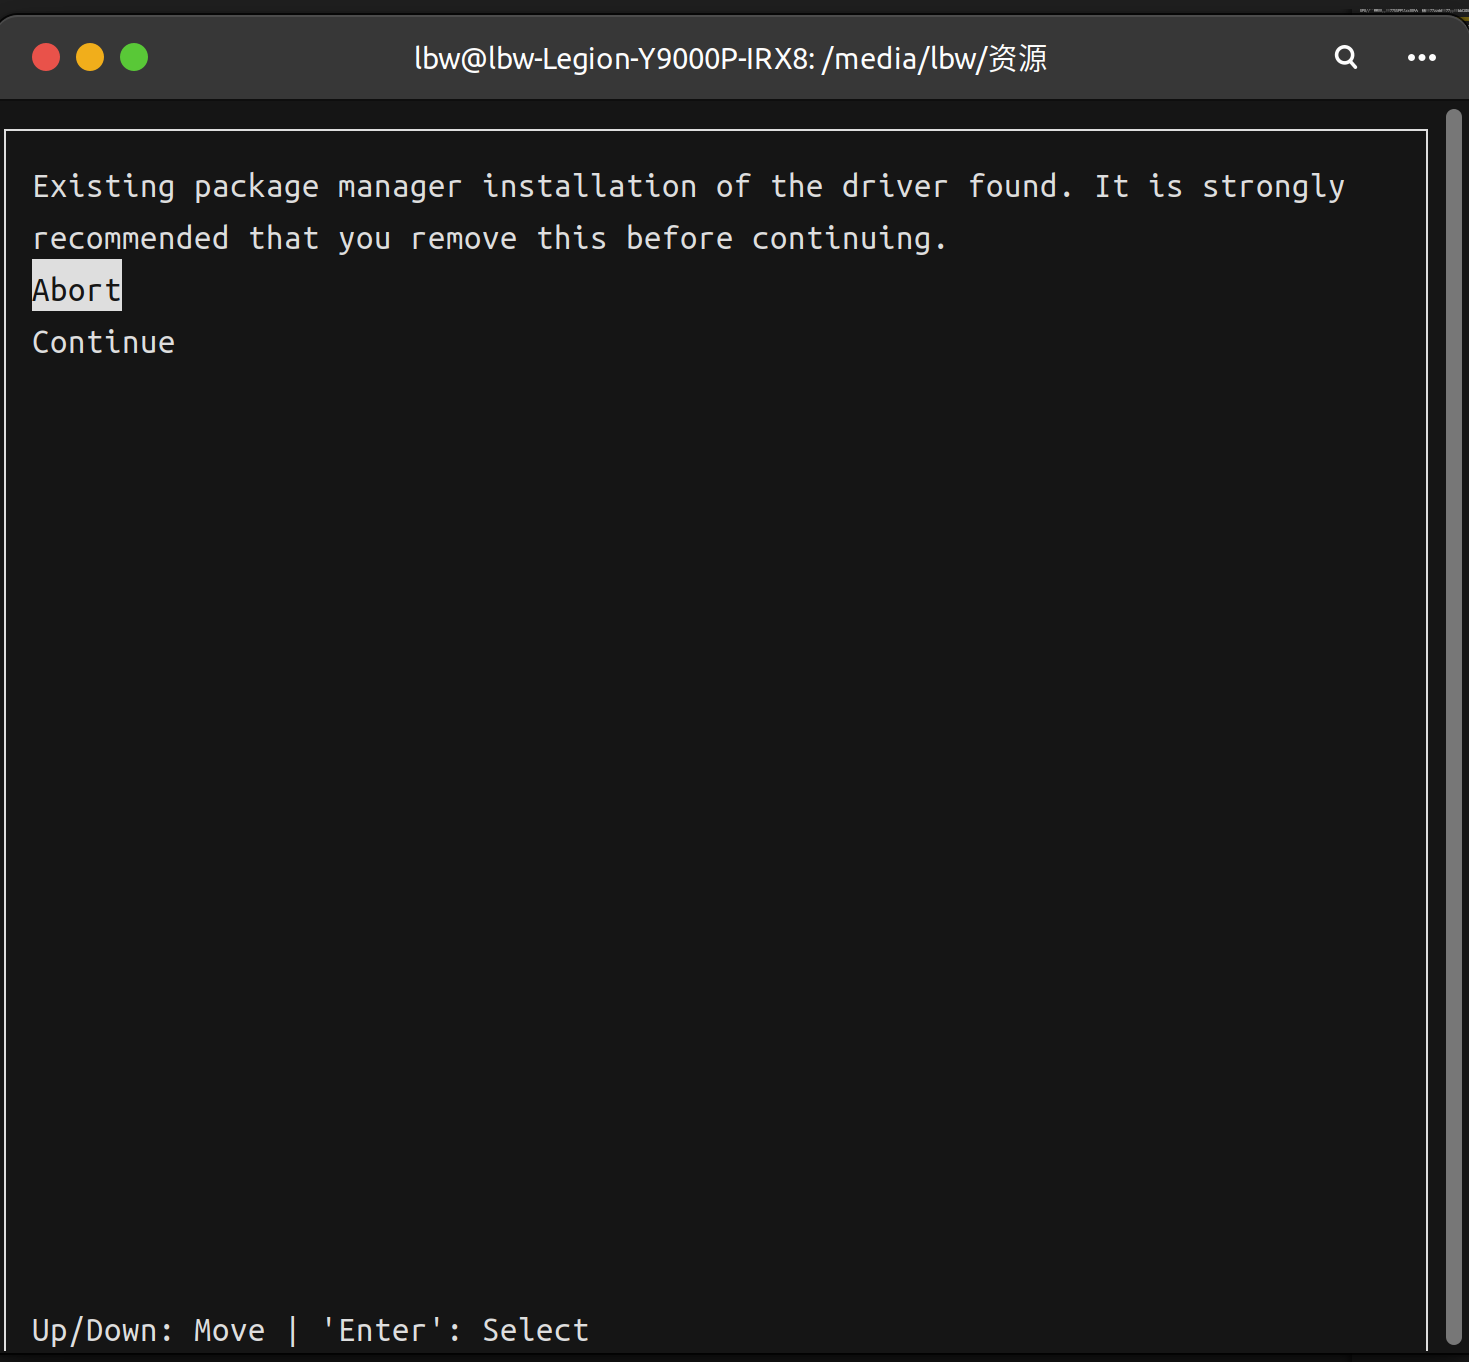
\includegraphics[width=0.7\textwidth]{CUDA_install.png}
    \caption{Step1} % 图片标题
    \label{fig:CUDA_install} % 图片标签,用于引用
\end{figure}

选择\textbf{Continue},

\begin{figure}[H]
    \centering
    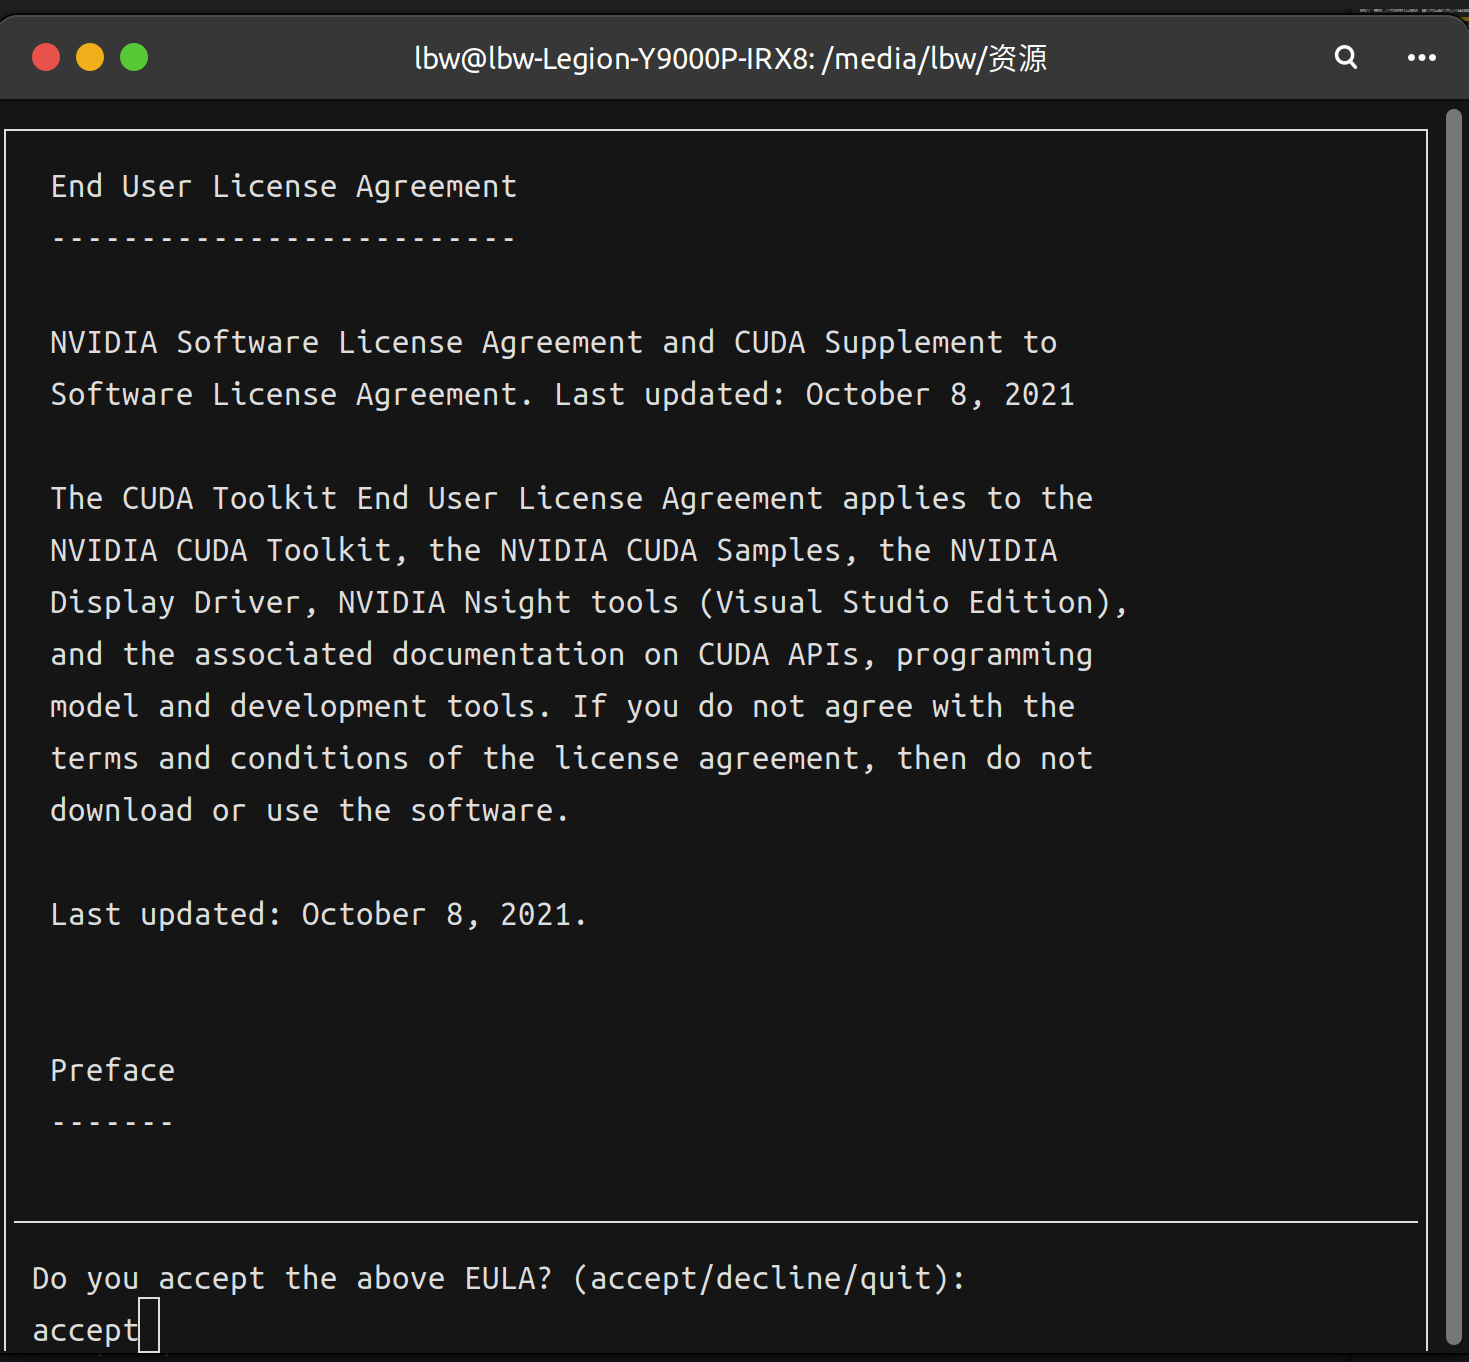
\includegraphics[width=0.7\textwidth]{CUDA_accept.png}
    \caption{Step2} % 图片标题
    \label{fig:CUDA_install} % 图片标签,用于引用
\end{figure}

输入\textbf{accept},进行下一步安装。

\begin{figure}[H]
    \centering
    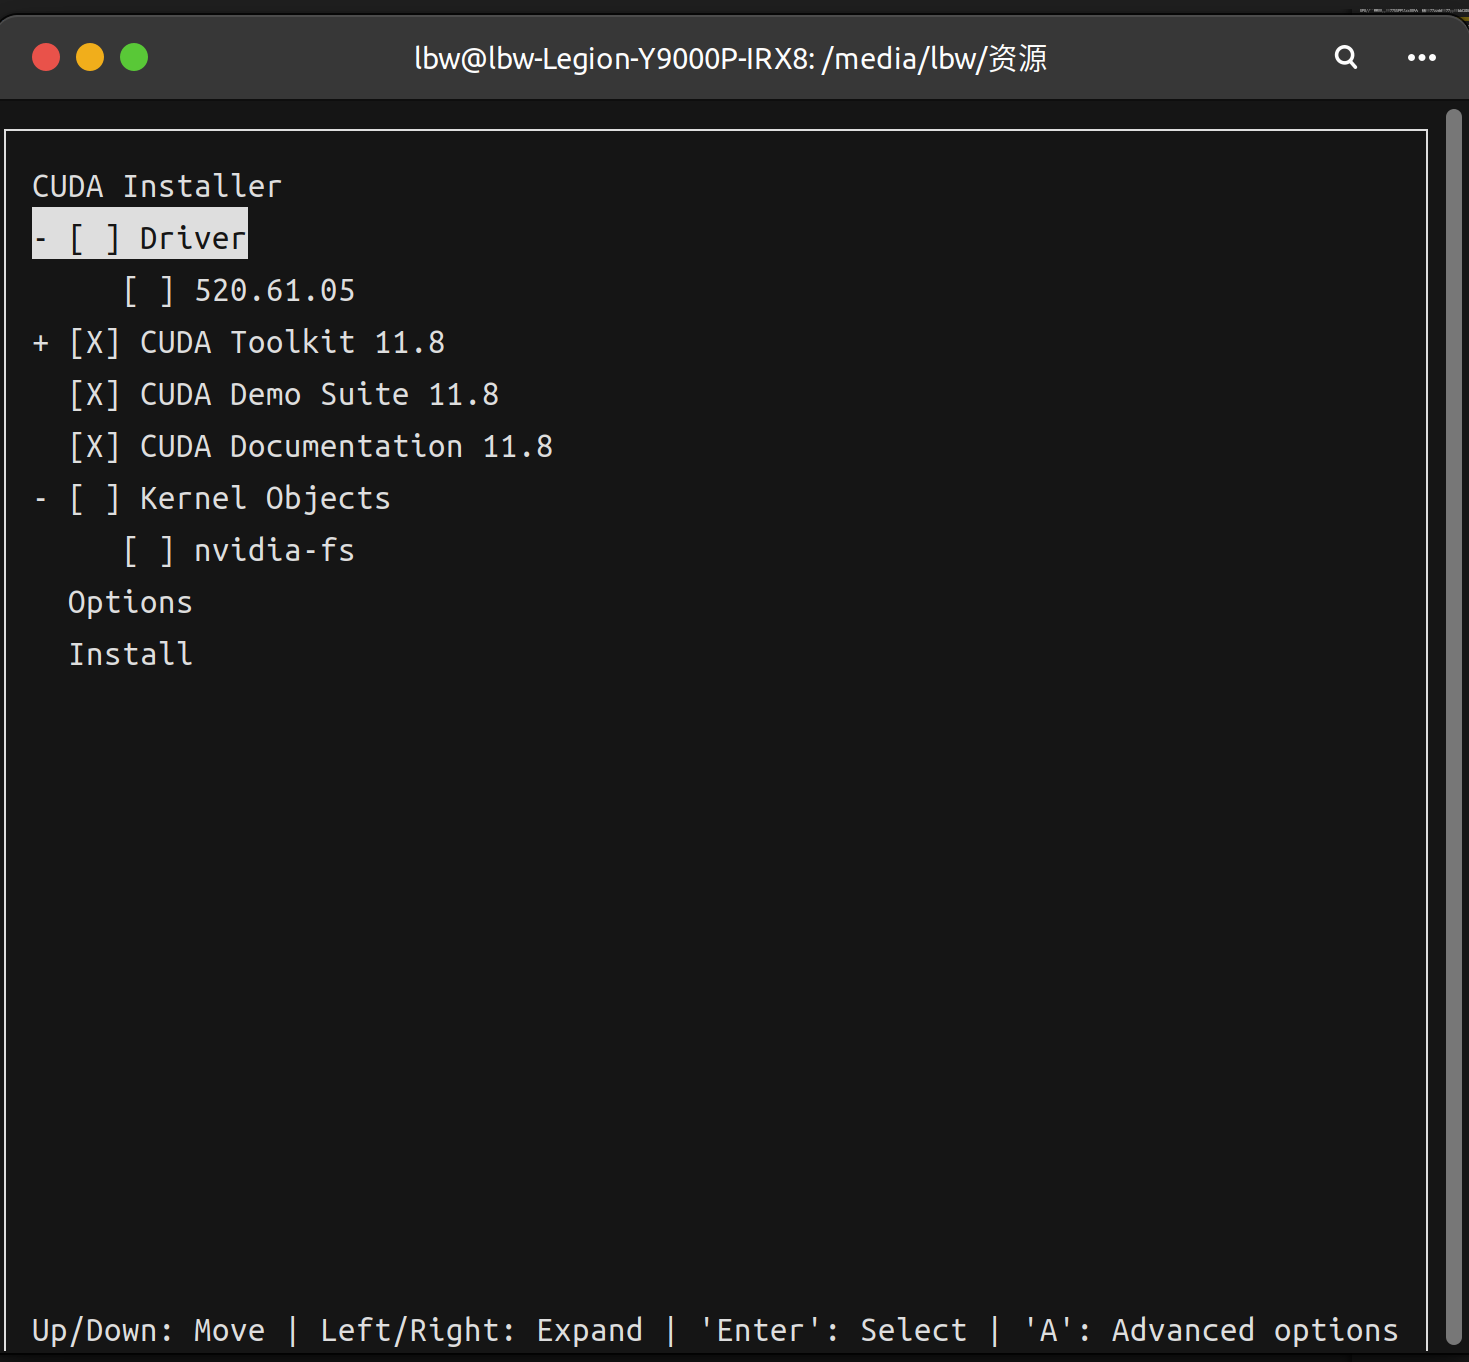
\includegraphics[width=0.7\textwidth]{CUDA_warning.png}
    \caption{Step3} % 图片标题
    \label{fig:CUDA_install} % 图片标签,用于引用
\end{figure}

这里需要特别注意,按下\textbf{Space}键,取消安装驱动,我们只安装toolkit。
\textbf{否则将会导致显卡掉驱动,严重者将导致屏幕无法亮起,请务必注意}。

完成后,请按照提示设置环境变量。然后就可以使用命令\textbf{nvcc}检测是否安装成功。

\begin{figure}[H]
    \centering
    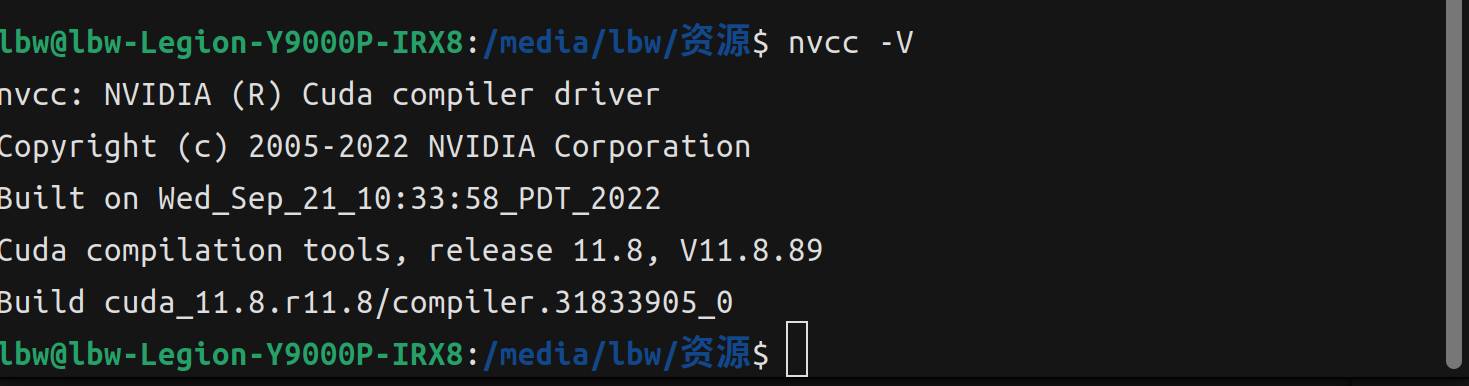
\includegraphics[width=0.7\textwidth]{CUDA_check.png}
    \caption{Step4} % 图片标题
    \label{fig:CUDA_install} % 图片标签,用于引用
\end{figure}

出现上图说明安装成功。

\subsubsection{安装cuDNN}

cuDNN是NVIDIA针对深度学习的深度神经网络加速库,可以加速卷积神经网络的运算。

推荐使用包解压的方式安装cuDNN,这样方便进行CUDA toolkit和cuDNN版本的管理。

\begin{tbash}
# 下载cuDNN安装包
wget https://developer.download.nvidia.com/compute/
redist/cudnn/v8.3.3/cudnn-11.8-linux-x64-v8.3.3.33.tgz

# 解压安装包
tar -xzvf cudnn-11.8-linux-x64-v8.3.3.33.tgz

# 移动cuDNN文件到CUDA安装目录
sudo cp cuda/include/cudnn*.h /usr/local/cuda/include
sudo cp cuda/lib64/libcudnn* /usr/local/cuda/lib64
sudo chmod a+r /usr/local/cuda/include/cudnn*.h /usr/local/cuda/lib64/libcudnn*
\end{tbash}

注意,只有在系统库中发现了cuDNN的库头文件和库文件,CUDA程序才可以正常使用。

\subsection{CUDA运行逻辑}

\subsubsection{异构计算架构}

GPU并不是一个独立运行的计算平台,而需要与CPU协同工作,可以看成是CPU的协处理器,CPU会对GPU进行任务下达和指令部署,因此当我们在说GPU并行计算时,其实是指的基于CPU+GPU的异构计算架构。

在异构计算架构中,GPU与CPU通过PCIe总线连接在一起来协同工作,CPU所在位置称为为主机端(host),而GPU所在位置称为设备端(device)

\begin{figure}[H]
    \centering
    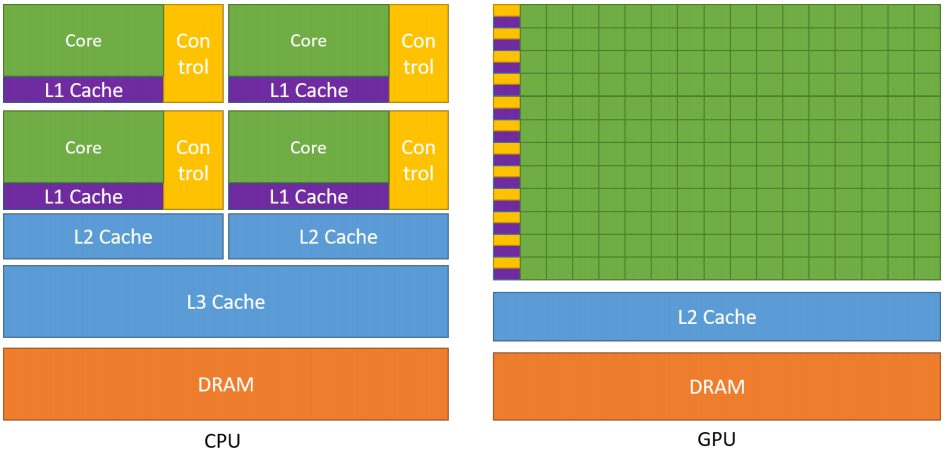
\includegraphics[width=0.85\textwidth]{Host-Device.png}
    \caption{CPU-GPU混合架构} % 图片标题
    \label{fig:CPU-GPU} % 图片标签,用于引用
\end{figure}

















\subsection{CUDA编程基础}
可以参考NVIDIA官方的CUDA编程指南\url{https://www.nvidia.cn/docs/IO/51635/NVIDIA_CUDA_Programming_Guide_1.1_chs.pdf}




\section{相机参数与成像原理*} 

在机器视觉算法中,有一个很重要又经常被忽略的部分。有些时候我们太关注算法的性能,但是忽略了相机的成像质量。“巧妇难为无米之炊”,如果相机成像的效果不好,那么再优秀的算法都无法发挥作用。
相机是机器视觉最重要的组成部分,它可以捕捉到周围环境的各种信息,并将其转换为图像。相机参数是相机的一些基本参数,如焦距、光圈、快门等。
了解相机参数和成像原理对于理解相机的工作原理非常重要。

\subsection{相机参数}
本小节将会结合相机的结构去介绍相机的各种参数。
\subsubsection{感光元件}
相机目前的主流的感光元件有CCD(电荷耦合)和CMOS(互补金属氧化物半导体)两种。

\textbf{CCD}

Charge Coupled Device,它使用一种高感光度的半导体材料制成,由许多感光单位组成,通常以百万像素为单位。当CCD表面受到光线照射时,每个感光单位会将电荷反映在组件上,即把光线转变成电荷,电荷在像素之间依次传递,最终集中到串联寄存器,转换为电压信号,然后放大,经模数转换后形成数字信号。而后数字信号,经过压缩后保存在相机内部的闪速存储器或内置硬盘卡中。有能力生产CCD 的公司分别为:索尼、飞利浦、柯达、松下、富士、夏普,大半是日本厂商。

\textbf{CMOS}

Complementary Metal-Oxide Semiconductor,和CCD一样同为在数码相机中可记录光线变化的半导体。CMOS的制造技术和一般计算机芯片没什么差别,主要是利用硅和锗这两种元素所做成的半导体,使其在CMOS上共存着带N(带–电) 和 P(带+电)级的半导体,这两个互补效应所产生的电流即可被处理芯片纪录和解读成影像。
每个像元都有独立的节点,转换为电压信号,然后放大,经模数转换后形成数字信号。

\textbf{CCD与CMOS的区别}

1.成像过程

CCD仅有一个(或少数几个)输出节点统一读出,其信号输出的一致性非常好。

CMOS中每个像素都有各自的信号放大器,各自进行电荷-电压转换,信号输出的一致性较差。

CCD为了读出整幅图像信号,要求输出放大器的信号带宽较宽。

CMOS中,每个像元中的放大器的带宽要求较低,大大降低了芯片的功耗,但数以百万的放大器的不一致性却带来了更高的固定噪声。

2.集成性

CCD中的电路和器件是集成在半导体单晶材料上,工艺较复杂。其仅能输出模拟电信号,需要后续的地址译码器、模数转换器、图像信号处理器处理,并且还需要提供三组不同电压的电源和同步时钟控制电路,集成度非常低。

CMOS能将图像信号放大器、信号读取电路、A/D转换电路、图像信号处理器及控制器等集成到一块芯片上,集成度高,芯片级相机的概念也由此产生。

3.速度

CCD采用光敏元输出,只能按规定的程序输出,速度较慢。

CMOS有多个电荷-电压转换器和行列开关控制,读出速度较快。此外,CMOS的地址选通开关可随机采样,实现子窗口输出,在仅输出子窗口图像时可获得更高的速度。

4.噪声

CCD采用PN结或二氧化硅隔离层隔离噪声,成像质量相对CMOS有一定的优势。

CMOS的集成度较高,各元件、电路之间距离很近,干扰较为严重,噪声对图片质量影响很大。

5.功耗

CCD需要3路电源来满足特殊时钟的需求,功耗较大。

CMOS只需一个电源供电,功耗仅为CCD的1/10。

\textbf{总结}

目前,市场销售的数码摄像头中以CMOS感光器件的为主。在采用CMOS为感光元器件的产品中,通过采用影像光源自动增益补强技术,自动亮度、白平衡控制技术,色饱和度、对比度、边缘增强以及伽马矫正等先进的影像控制技术,完全可以达到与CCD摄像头相媲美的效果。

受市场情况及市场发展等情况的限制,摄像头采用CCD图像传感器的厂商为数不多,主要原因是采用CCD图像传感器成本高的影响,同时由于CCD耗电量大,工艺复杂,像素提高难度加大。

\subsubsection{相机感光参数}
调整相机对环境的感光程度,主要有以下三个途径,分别是光圈、快门和ISO。

\textbf{光圈}

通过调整镜头光圈的大小,调整进光量,光圈大小有两种写法:大F写法(F2.8)、小f写法(f/2.8),两种写法完全等价,例如F4指的是光圈大小占镜头直径的4分之1。
F后面的数字越大,光圈越小,反之则反。

1.挡位设计

光圈的档位设计是相邻的两档的数值相差1.4倍(2的平方根1.414的近似值)相邻的两档之间。
透光孔直径相差根号2倍,透光孔的面积相差一倍, 底片上形成的影像的亮度相差一倍,维持相同曝光量所需要的时间相差一倍。

所有的光圈挡位有:

f/1.0,f/1.4,f/2.0,f/2.8,f/4.0,f/5.6,f/8.0,f/11,f/16,f/22,f/32,f/44,f/64

2.光圈分类

固定光圈:最简单的相机只有一个园孔的固定光圈

沃特侯瑟光圈:最初的可变光圈只是一系列大小不同的园孔排列在一个有中心轴的圆盘的周围;转动园盘可将适当大小的圆孔移到光轴上,达到控制孔径的效果。十九世记中叶约翰·沃特侯瑟发明这种光圈。

猫眼式光圈:由一片中心有椭圆形或菱形孔的金属薄片平分为二组成,将两片有半椭圆形或半菱形孔的金属薄片对排,相对移动便可形成猫眼式光圈。猫眼式光圈多用于简单照相机。

"虹膜"式光圈:是由多个相互重叠的弧形薄金属叶片组成的,叶片的离合能够改变中心圆形孔径的大小。有些照相机可以借助转动镜头筒上的圆环改变光圈孔径的大小,而有些照相机则是利用微处理器芯片控制微电机自动地改变光圈的孔径。弧形薄金属叶片可多达十八片。弧形薄金属叶片越多,孔径越近圆形。通过电子计算机设计薄金属叶片的形状,可以只用7片薄金属叶,得到近圆形孔径。

瞬时光圈:单反照相机的光圈是瞬时光圈,只在快门开启的瞬间,光圈缩小到预定大小。平时光圈在最大位置。

兼快门光圈:有的简便照相机的光圈兼有快门的功能,这类兼快门光圈大多是双叶片的猫眼式光圈,与单纯猫眼式光圈不同的是:于兼快门光圈平时是完全关闭的:在按下快门的瞬间,双叶片光圈开启到预定的孔径后,保持这孔径到一段预定快门开启时间之后,立刻闭合:如此一来,光圈便又兼快门的功能。

偷懒不放图了先(逃

\textbf{快门}

快门是遮光板,只有当快门打开的时候,底片才能接收到光照。所以快门可以控制进光时间。
快门越块:成像时间越短,被拍摄物品移动的距离越小,图像越清晰。常用于静态拍摄。
反之则反

但是随着相机技术进步,现在相机大部分使用电子快门,常见的电子快门主要有两种,卷帘快门和全局快门

1.卷帘快门

卷帘快门通过逐行扫描的方式从上到下捕获图像,而不是一次性捕获所有像素。这意味着每一行像素的曝光存在微小的时间差。当相机或物体高速移动时,这种逐行扫描可能导致图像失真,形成“果冻效应”
但是其有着成本低,分辨率高的优点,使其在一些需要高分辨率但对动态性能要求不高的应用中非常适用,如静态图像捕捉或家用监控。

卷帘快门导致的果冻效应,其显著程度主要取决于以下几个因素:

*物体的移动速度:移动速度越快,失真越明显。

*物体的大小:大尺寸物体在画面中的扭曲更加明显。

*分辨率:更高的分辨率在相同帧率下行时间更短,相对可以减少失真。

2.全局快门

全局快门(Global Shutter)是一种图像传感器技术,其核心在于能够同时捕获画面中所有像素的信息。与逐行扫描的滚动快门不同,全局快门的所有像素在同一时间曝光,然后一起读取数据,这种同步曝光方式使其在高速运动场景中能够有效消除图像失真现象,如“果冻效应”(rolling shutter effect)。可以将其比作拍照时快门在一瞬间“拍下”整个画面,而非逐行扫描捕捉,确保每一部分都与真实场景一致。

\begin{figure}[H]
    \centering
    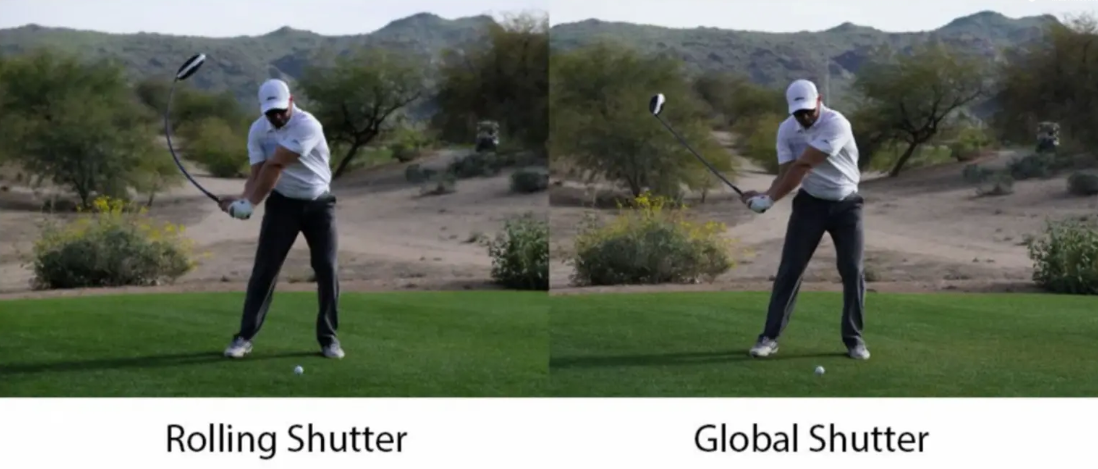
\includegraphics[width=0.7\textwidth]{rolling_shutter.png}
    \caption{快门对比} % 图片标题
    \label{fig:果冻} % 图片标签,用于引用
\end{figure}

总结

静态场景可以使用卷帘快门相机,相同价格下,可以获得更高分辨率的相机,动态场景下,则需要根据情况权衡,优先全局快门相机,其次高帧率,高分辨率的
卷帘快门,在要求不高的程度上,也可以,请根据成本酌情考虑。在笔者眼里,全局快门的缺点就是贵(哭

\textbf{ISO}

感光度,又称为ISO值,是衡量底片对于光的灵敏程度。
对光越灵敏,越适合捕捉暗光线:亮处用小ISO即可,暗处用大ISO。对光越灵敏,意味着所需的进光时间越短:
意味着所需快门的时间越短。所以ISO值上限决定了快门的上限,只有ISO足够大,快门才可以足够快。
意味着曝光量越少。所以ISO越大,图像越模糊,使用较高敏感度通常会导致影像质量降低(较粗的底片颗粒或是较高的影像噪声)。
ISO每差一倍,曝光量差一档,也就是说相差一档光圈或者一档快门。

提高ISO会降低图像质量,所以优先采取其他方法提高亮度。

\subsubsection{图片噪点}
噪点在图像上常表现为一引起较强视觉效果的孤立像素点或像素块。比如上午所提的提高ISO或者相机长时间工作过热等,都可能会导致出现噪点。

图像常见噪声基本上有以下四种,高斯噪声,泊松噪声,乘性噪声,椒盐噪声。

\begin{figure}[H]
    \centering
    \includegraphics[width=0.6\textwidth]{raw.png}
    \caption{原图} % 图片标题
    \label{fig:原图} % 图片标签,用于引用
\end{figure}

\textbf{高斯噪声}

高斯噪声是指它的概率密度函数服从高斯分布(即正态分布)的一类噪声。如果一个噪声,它的幅度分布服从高斯分布,而它的功率谱密度又是均匀分布的,则称它为高斯白噪声。高斯白噪声的二阶矩不相关,一阶矩为常数,是指先后信号在时间上的相关性。

产生原因:

1)图像传感器在拍摄时市场不够明亮、亮度不够均匀。

2)电路各元器件自身噪声和相互影响。

3)图像传感器长期工作,温度过高。

\begin{figure}[H]
    \centering
    \includegraphics[width=0.6\textwidth]{gaussian.png}
    \caption{高斯噪声} % 图片标题
    \label{fig:高斯噪声} % 图片标签,用于引用
\end{figure}

\textbf{泊松噪声}

泊松噪声,就是符合泊松分布的噪声模型,泊松分布适合于描述单位时间内随机事件发生的次数的概率分布。如某一服务设施在一定时间内受到的服务请求的次数,电话交换机接到呼叫的次数、汽车站台的候客人数、机器出现的故障数、自然灾害发生的次数、DNA序列的变异数、放射性原子核的衰变数等。

\begin{figure}[H]
    \centering
    \includegraphics[width=0.6\textwidth]{poisson.png}
    \caption{泊松噪声} % 图片标题
    \label{fig:泊松噪声} % 图片标签,用于引用
\end{figure}

\textbf{乘性噪声}

乘性噪声一般由信道不理想引起,它们与信号的关系是正相关,信号在它在,信号不在他也就不在。

\begin{figure}[H]
    \centering
    \includegraphics[width=0.6\textwidth]{x.png}
    \caption{乘性噪声} % 图片标题
    \label{fig:乘性噪声} % 图片标签,用于引用
\end{figure}

\textbf{椒盐噪声}

椒盐噪声,椒盐噪声又称脉冲噪声,它随机改变一些像素值,是由图像传感器,传输信道,解码处理等产生的黑白相间的亮暗点噪声。

\begin{figure}[H]
    \centering
    \includegraphics[width=0.6\textwidth]{salt.png}
    \caption{椒盐噪声} % 图片标题
    \label{fig:椒盐噪声} % 图片标签,用于引用
\end{figure}

\subsubsection{相机图片储存格式}
\textbf{1.Bayer格式}

bayer格式图片是伊士曼·柯达公司科学家Bryce Bayer发明的,Bryce Bayer所发明的拜耳阵列被广泛运用数字图像处理。

bayer 格式图片在一块滤镜上设置的不同的颜色,通过分析人眼对颜色的感知发现,人眼对绿色比较敏感,所以一般bayer格式的图片绿色格式的像素是是r和g像素的和。

另外,Bayer格式是相机内部的原始图片, 一般后缀名为.raw。很多软件都可以查看, 比如PS。我们相机拍照下来存储在存储卡上的.jpeg或其它格式的图片, 都是从.raw格式转化过来的。如下图,为bayer色彩滤波阵列,由一半的G,1/4的R,1/4的B组成。

Bayer格式的图片是单通道的。

\textbf{2.RGB格式}

RGB格式是一种多通道图像格式,它将图像分为三个通道,分别为红色通道、绿色通道、蓝色通道。

RGB格式的特点是:

1.每个像素点由三个相邻像素点组成,分别对应三个通道。


RGB格式的优点是:

1.RGB格式的图像可以同时处理红色、绿色、蓝色通道,可以提高图像处理速度。

2.RGB格式的图像占用空间小,占用内存小。

RGB格式的缺点是:

对场景的光照和颜色变化比较敏感,不适用一些需要保持颜色稳定性的应用场景。

\subsubsection{相机伽马值}

所谓伽玛校正就是对图像的伽玛曲线进行编辑,以对图像进行非线性色调编辑的方法,检出图像信号中的深色部分和浅色部分,并使两者比例增大,从而提高图像对比度效果。计算机绘图领域惯以此屏幕输出电压与对应亮度的转换关系曲线,称为伽玛曲线(Gamma Curve)。

在不使用伽马校正去产生JPG图像意味着亮度等级水平在进行8位的转换时会有一定的损失,就会产生“台阶”效果。通过调校亮度的分布就是进行伽马校正意味着那些效果会得到补偿修复。gamma校正的意义就在于将人眼感受到的灰度值, 转换到自然界真正的灰度值(因为人不是测量器, 人只能感受和比较)

\textbf{gamma校正原理}

假设图像中有一个像素,值是 200 ,那么对这个像素进行校正必须执行如下步骤: 
  1. 归一化 :将像素值转换为 0 ~ 1 之间的实数。算法如下:( i + 0. 5)/256 这里包含 1 个除法和 1 个加法操作。对于像素 A 而言,其对应的归一化值为0. 783203 。 

  2. 预补偿 :根据公式, 求出像素归一化后的 数据以1/gamma为指数的对应值。这一步包含一个求指数运算。若gamma值为2. 2 ,则1 /gamma为0. 454545 , 对归一化后的A值进行预补偿的结果就是0. 783203 \^ \ \ \   0. 454545 = 0. 894872。 

  3. 反归一化 :将经过预补偿的实数值反变换为0~255之间的整数值。具体算法为 : f*256 - 0. 5  此步骤包含一个乘法和一个减法运算。续前例, 将A的预补偿结果0. 894872代入上式, 得到A预补偿后对应的像素值为  228 , 这个  228  就是最后送 入显示器的数据。

  
  如上所述如果直接按公式编程的话,假设图像的分辨率为 800*600 ,对它进行 gamma 校正,需要执行 48 万个浮点数乘法、除法和指数运算。效率太低,根本达不到实时的效果。 
  针对上述情况,提出了一种快速算法,如果能够确知图像的像素取值范围,例如, 0 ~ 255 之间的整数  , 则图像中任何一个像素值只能 是  0  到  255  这  256  个整数中的某一个 ; 在  gamma 值 已知的情况下  ,0 ~ 255  之间的任一整数  , 经过“归一 化、预补偿、反归一化”操作后 , 所对应的结果是唯一的  , 并且也落在  0 ~ 255  这个范围内。
  如前例, 已知gamma值为2. 2,像素A的原始值是200,就可求得经gamma校正后A对应的预补偿值为  228 。基于上述原理  , 我们只需为  0 ~ 255  之间的每个整数执行一次预补偿操作  , 将其对应的预补偿值存入一个预先建立的  gamma  校正查找表 (LUT:Look Up Table) , 就可以使用该表对任何像素值在  0 ~ 255  之 间的图像进行  gamma  校正。
 
\begin{figure}[H]
    \centering
    \includegraphics[width=0.95\textwidth]{gamma.png}
    \caption{伽马矫正} % 图片标题
    \label{fig:伽马矫正} % 图片标签,用于引用
\end{figure}

\subsubsection{相机景深}
景深(depth of field)定义:摄影机镜头或其他成像器前沿能够取得清晰图像的成像所测定的被摄物体前后距离范围。通俗讲即被拍摄物体对焦点(focus point)平面处的景物,在胶片上会形成清晰影像,在对焦点平面的前方某处到其后方某处有一个范围,其内的景物都能形成清晰影像,这一范围称为景深,讨论景深,一般我们用“深浅”形容,即浅景深(narrow depth of field)或大景深(large depth of field)。

\textbf{景深的原理}

理解景深原理前,我们必须明白一件事:当我们对焦时,其实只有一个平面是真正合焦的。这个平面与像平面(可以简单理解为胶片或者传感器平面)平行。凡是在这个平面之前或者之后的都不是合焦状态。合焦平面上物体某点发出不同角度的光在像平面成像都汇聚于一点,而非合焦物体的某点发出不同角度的光会落在像平面不同点上,形成一个模糊圆,这个圆术语叫做弥散圆(circle of confusion)。

\begin{figure}[H]
    \centering
    \includegraphics[width=0.95\textwidth]{diffuse_circle.png}
    \caption{弥散圆} % 图片标题
    \label{fig:弥散圆} % 图片标签,用于引用
\end{figure}
如果弥散圆小到人眼无法鉴别(或者说弥散圆直径小于传感器像元的大小),模糊圆可被视为点的成像,看起来就和对上焦的东西一样清晰,此无法分辨的弥散圆称为容许弥散圆(permission circle of confusion)。在被摄物体(对焦点或合焦平面)前后纵深,有一段距离,其影像在像平面的模糊程度肉眼无法分辨,比较清晰,都在容许弥散圆限定范围内,它们之间距离称为景深。

\textbf{*景深的计算}

\begin{figure}[H]
    \centering
    \includegraphics[width=1\textwidth]{depth_of_field.png}
    \caption{景深计算} % 图片标题
    \label{fig:景深计算} % 图片标签,用于引用
\end{figure}
可见,前景深,小于后景深。
\begin{figure}[H]
    \centering
    \includegraphics[width=0.95\textwidth]{simple.png}
    \caption{景深简化计算} % 图片标题
    \label{fig:景深简化计算} % 图片标签,用于引用
\end{figure}
\textbf{景深的影响因素}

镜头光圈:光圈越大,景深越小;光圈越小,景深越大;

镜头焦距:镜头焦距越长,景深越小;焦距越短,景深越大;

拍摄距离:距离越远,景深越大;距离越近,景深越小。
\begin{figure}[H]
    \centering
    \includegraphics[width=0.75\textwidth]{aperture.png}
    \caption{光圈} % 图片标题
    \label{fig:光圈} % 图片标签,用于引用
\end{figure}
\subsubsection{焦段的选择}



相机镜头的选择

镜头参数

光圈大小之类的

\subsection{相机畸变模型}
\subsubsection{针孔相机}
\subsubsection{鱼眼相机}
\subsubsection{广角相机}

相机标定介绍
几种常用的标定板/棋盘,圆点,aruco,charuco

ros包标定 opencv标定 手写标定
每种给出文档,手写标定研究一下,写出来给

单目标定,双目标定,动态标定,在线标定,自标定(这两个有区别),无标定板标定等多种类型的标定

\subsubsection{相机选购}
几种常见的相机像素单位,商家说高清,不一定真高清

相机帧率不一定是当前的分辨率,可能指的是120hz的时候480p,1080p的时候其实只有30hz

分清黑白,分辨率等参数

定焦,自动调焦AF/FF

\subsection{HDR实现}
\subsection{多相机同步}


\section{信号处理与滤波器*}
在前端的成像和识别过程中,由于或多多少的原因,信号会发生一些变化,也会产生大量的噪声。如何滤除这些噪声,对于算法决策的准确性至关重要,在本章节我们将学习一些滤波器的基本知识。
并且运用我们学习到的知识,去自主设计一些滤波器,并将其应用到我们的算法中。

\section{导航技术初步*}
对于一个智能机器人来说,获取周围环境和自身情况的能力是至关重要的。导航技术是其核心技术之一。在本章节中,我们将了解激光雷达的工作原理,并学习一些基本的导航算法,并将其应用到我们的机器人中。

现在,你坐在哨兵的脑袋里面,你的目标是悄悄摸到敌方基地后面偷家。
但是没认真看规则的你忘记了地图长什么样,你打开手机,发现好心的wzx部长已经帮你存了一份\textbf{标准赛场地图[1]}。
于是你打开\textbf{缺德地图[2]},把赛场地图传上去。你又打开手机GPS,把自己的\textbf{定位[3]}也告诉缺德地图,
最后,你输入目的地,缺德地图就帮你规划好了一条用时最少的路。
于是你就跟着这条路径走,同时你并没有关掉GPS,这样才知道自己有没有走错。
在路上,你在\textbf{视野[4]}里看到了许多其他机器人,你以你秋名山车神的\textbf{车技[5]},在他们之间穿梭,避开了所有车。
突然!What can I say, man!无人机坠机坠在了你前进的道路上。
你对车身大小了如指掌。只看一眼,你计算出哨兵过不去,路被堵了。
鉴于无人机死状惨烈,这无人机短时间是飞不起来,你走不了这条路了。
不过还好,每隔一段时间,缺德地图会再算一次路径,你可能会听到“正在为您重新规划路径”,他帮你找到了另一条路。
虽然“缺德地图持续为您服务”,但是有时候你可能会开到一些“信号不好”,无法获取缺德地图服务的地方。
此时,你要能够在不依靠缺德地图的情况下\textbf{自己找到[6]}信号比较好能重新连接上缺德地图服务的地方。
最终你成功到达了目的地。

\begin{figure}[H]
    \centering
    \includegraphics[width=0.8\textwidth]{./images/Nav2导航框架.png}
    \caption{map}
    \end{figure}
从上面可以看出,导航需要:

\textbf{[1]地图(全局代价地图Global Costmap)}

\textbf{[2]导航系统(全局规划器Global Planner)}

\textbf{[3]定位系统(多传感器融合定位)Sensor Transform}

\textbf{[4]附近的视野(局部代价地图Local Costmap)}

\textbf{[5]车手(局部规划器Local Planner)}

\textbf{[6]应急方案(恢复行为树Recovery Behavior Tree)}

因此,导航的工作流程就是:

通过传感器数据与全局地图匹配,获得自身在地图的坐标;
根据目标坐标,利用全局规划器算出路径;
实时更新自身定位,并将扫描到的障碍物信息融合到局部代价地图中;
根据局部代价地图,利用局部规划器算出车各个方向的速度应该是多少,发给下位机;
如果遇到特殊情况则进入恢复行为树,暂停部分服务,直到脱离特殊情况;
根据规定的时间间隔(或情况),重新获取定位和目标,规划全局路径,并一直循环。

导航最重要的技术就是
\textbf{SLAM(simultaneous localization and mapping,实时定位和建图技术)}简称SM(不是)。
该技术的基础就是定位。但是可怜的小哨兵并没有GPS。
所以他只能用其他的定位技术,比如激光雷达、IMU、里程计、视觉相机等。
在ROS中,我们使用tf(transform)来表示坐标。frame是坐标系,tf的原理就是通过表示坐标系之间的关系来确定各个坐标系之间的相对位置。
常用的frame有:
\begin{itemize}
\item map:世界坐标系
\item odom:里程计坐标系
\item base\_link:小哨兵的坐标系
\item camera\_link:相机坐标系
\item laser\_link:激光雷达坐标
\item imu\_link:IMU坐标系
\item ...
\end{itemize}

tf的主要信息包含父子节点(及两个坐标系)之间由xyz表示的平移关系和四元数表示的旋转关系。
多个父子节点的tf可以组成一个tf树,树的根节点一般是map,树的叶子节点一般是各个传感器的坐标系。
通过tf树可以算出任意两个节点之间的坐标关系(相对位置)。

\subsection{\quad 激光雷达定位}
先简单介绍一下激光雷达的工作原理:激光雷达的工作原理是通过发射一束激光,然后接收到反射回来的信号,通过解码,得到反射点的坐标,根据反射光的强弱还能获得强度信息。

激光雷达定位主要分为四步:
\begin{enumerate}
\item 所有定位方法开始,都要先要有一张已有的地图,地图上记录了各个障碍物的位置、大小、置信度等信息。将地图上的某一点设为原点,以原点为中心展开的坐标系为map坐标系。
\item 激光雷达扫描四周环境,得到一张激光雷达“视野内”的地图,上面记载了周围的障碍物信息(更多细节将在下一节详细介绍)
\item 将这张地图与已有的地图进行对比匹配,得到雷达最可能存在的位置,将该位置与map坐标系之间的相对位置变化记为map与ladar之间的tf。
\item 结合laser与baselink之间的tf(一般是提前固定写好的,由雷达固定在车体的位置和朝向决定),得到baselink与map之间的相对位置变化,即得到小哨兵在map坐标系下的位置。
\end{enumerate}
其中匹配方式大体可分为两种:二维和三维匹配。

二维匹配:将三维的点云信息按一定规则压缩到二维(二向箔),获得附近的实时的二维地图,与已有的地图进行匹配(如AMCL算法)。地图为栅格地图(即用像素表示地图,灰度表示障碍物置信度,支持pgm,png,jpg格式,可手动PS修改)。

三维匹配:直接将扫描到的点云与之前存储的点云匹配,定位更准确,但是匹配速度慢(如ICP,NDT匹配算法)。常会用到kd-tree,oct-tree等数据结构加速匹配。一般与先前一小段时间内的储存的点云进行匹配,获得相对移动,是一种动态的匹配。
因此需要将较久之前扫描到的点云,或者距离较远的点云从kdtree之类的数据结构中清理掉,防止匹配目标过大。(point-lio里的$fov\_segment()$函数就是干这个的所以不能删掉@wzx)

运动过程中多用动态的匹配,以便较快的更新定位,提高实时性。与整张全局地图的匹配,一般在特定情况下(如刚开机上电不知道自己在哪的时候;定位可能出现偏差的情况;或者执行完恢复行为之后。也可以时不时重定位一下,上赛季就是这么干的,效果好像不太行QAQ)才进行,又叫重定位,即直接清零更新baselink和map之间的tf。
\subsection{\quad 里程计,IMU定位}
里程计定位较为简单,直接获取机器人各个方向运动的里程,加在map坐标系下的位置即为小哨兵的位置。
IMU,即惯性测量单元,可以测量各方向的角速度和线加速度,通过积分,获得类似里程计的数据,加在map坐标系下的位置即为小哨兵的位置。

\subsection{视觉定位}
视觉定位也是近年来较为流行的SLAM技术,它与激光雷达定位类似,但他获取的特征信息在相同情况下比激光雷达多。
它通过提取图像中的特征点(一般是角点),与原先存储的地图里的特征点对比匹配,计算出相机的相对位移,累加后得到小哨兵在map坐标系的坐标变换。

\subsection{多传感器融合}
以上各个定位方法都有自己的局限性:
\begin{itemize}
\item imu,里程计定位:由于IMU和里程计对运动(速度,加速度)测量的精度较高,定位较为准确。但由于其本身稳定性较差,易受干扰(如IMU受热噪声干扰的零漂,轮式里程计打滑等情况);
        且他们都是“开环”的测量方式,一旦出现意外情况(比如受干扰,或者某些情况下超过其测量范围(比如被别的机器人肘了一下,瞬时加速度太大IMU测量不了)),
        测量的位置歪掉了,就再也回不来了,因为没法校正。
\item 视觉定位:视觉定位的精度较低,且受相机的分辨率、光照、遮挡等因素影响较大。且对需要物体纹理较多效果才比较好。
\item 雷达定位:激光雷达只能获取深度信息,这会导致在一些特殊情况中定位失效。
        如雷达在非常长的两堵一模一样的墙之间前进,虽然车在前进,但在雷达的视野里,左右离墙的距离不变,而前后因为超出探测距离所以数据也不变,他就以为自己没有运动了;
        又如雷达在一个一个正方形房间的正中心,你趁雷达不注意(即在两次雷达扫描的间隔之间),把他旋转90度。在雷达的视野里,前后左右的障碍物与之前的完全相同,所以他会以为自己没旋转。
\end{itemize}
为了解决这些问题,人们将多种传感器的数据融合在一起得到更准确定位方法。

最常见的融合方法(也是我们现在使用的方法)是激光雷达和里程计的融合。
我们新建一个节点Odom,他作为map的子节点,作为base\_link的父节点。
雷达输出odom到baselink的tf,而map到odom的tf作为校正数值记录,如里程计与雷达数据的偏差等。
这样,小哨兵的位置就通过激光雷达和里程计 fusion 的方式得到。

其他的融合方法还有:激光雷达与视觉融合,将点云与图像匹配,使点云除了位置信息外,还能拥有颜色等信息。


导航需要地图。


我们使用的是二维地图(毕竟小哨兵还没学会飞行,在z轴上运动能力为0(其实还有roll和pitch),而且二维导航相关的导航,定位,建图方案都比较成熟)

\subsection{地图的获取}
首先,我们接收激光雷达扫描到的点云图,然后对其进行处理,压缩到二维,得到地图。

处理的第一步是进行点云的滤波。下面是一些常用的滤波方法:
\textbf{*注意:因为点云是通过物体表面反射光信息获取的,所以一个实体只有表面会有点云,内部是没有的。}
\begin{enumerate}
\item \textbf{Voxel滤波}:因为我们用的激光雷达比较牛逼,获得的近处点云比较稠密(保证远处的分辨率),这样直接计算会导致计算量过大,
所以我们可以将点云按照空间分辨率进行分割,又叫体素网格下采样。
\begin{tcode}
    pcl::VoxelGrid<pcl::PointXYZ> voxfilter;
    voxfilter.setInputCloud(cloud);
    // 设置滤波器的体素大小
    voxfilter.setLeafSize(0.1, 0.1, 0.1);
    voxfilter.filter(*cloud);
\end{tcode}
这样,我们就将cloud里每个0.1m*0.1m*0.1m的体素(三维空间中的一个小立方体单元)内的点替换为该体素的中心点。
将临近的点聚合到一个体素中来实现,可以减少点云数据的复杂度,同时保留整体的形状和结构。
\item \textbf{直通滤波}:直通滤波就是最简单的剔除不需要点云的滤波方法。比如小哨兵小小的,对它来说50cm以上的障碍物根本不影响他通过,那我们就可以把0.5m以上的点剔除掉。
\begin{tcode}
    pass_through_filter_z_.setFilterFieldName("z");
    pass_through_filter_z_.setFilterLimits(min_z, max_z);
    pass_through_filter_z_.setFilterLimitsNegative(false);
    pass_through_filter_z_.setInputCloud(input_cloud);
    pass_through_filter_z_.filter(*input_cloud);
\end{tcode}
这样,我们就将cloud里的z轴坐标在min\_z和max\_z之外的点剔除掉了。
同样的道理,还可以通过设置xy范围,把远处的,懒得考虑的点剔除掉。以及设置剔除一定半径内的点云,把哨兵本体的点云剔除掉。
\item \textbf{统计滤波}:在点云处理中,统计滤波是一种用于识别和移除离群点的方法,这些离群点可能是由于测量误差或噪声引起的。
该方法基于假设,即点云数据中的大部分点是符合高斯分布的,而离群点则是那些与这种分布显著不同的点。
\begin{tcode}
    pcl::StatisticalOutlierRemoval<pcl::PointXYZ> sor;
    sor.setInputCloud(cloud);
    // 设置近邻点的数量
    sor.setMeanK(50); 
    // 设置标准差倍数阈值
    sor.setStddevMulThresh(1.0); 
    // 设置为false表示移除离群点,设置为true表示保留离群点
    sor.setNegative(false); 
    sor.filter(*cloud);
\end{tcode}
通过这种方式,我们可以计算每个点到其K个最近邻点的平均距离,并根据这个平均距离与全局平均距离的比较来确定是否为离群点。
如果一个点的平均距离超过了全局平均距离加上标准差倍数的阈值,那么这个点就被认为是离群点并被移除。
这样可以有效地减少点云中的噪声和异常值,提高后续处理的准确性和效率。

\item \textbf{特殊方法滤波}:有时候一些特殊的物体需要滤掉,这时候就要自己编写特定的代码剔除。比如地板,是的,地板也是实体,也会产生点云,但他不是障碍物,所以需要过滤掉。
我们可以简单的通过直通滤波,把z轴坐标在0.1m以下的点剔除掉。也可以通过聚类(即将点云数据中的点根据它们的空间位置或属性特征分组),将最大的聚类剔除掉,这样就剔除了地板。
而我们现在用的是tc学长写的法向量剔除法,计算每个点的法向量,然后剔除法向量与z平面夹角小于一定角度的点(通俗来说:平的就是地板)。
\end{enumerate}



\subsection{全局规划器}

全局规划器是ROS中的核心模块之一,它负责规划机器人的全局路径,即从起始点到目标点的路径。
全局规划器的主要功能是生成一个全局路径,该路径是机器人从起始点到目标点的最短路径。
全局规划器的实现需要考虑机器人的移动方式、障碍物、地图等信息,以生成一个全局路径。

ROS中的全局规划器主要有两种实现方式:一种是基于RRT算法的全局规划器,另一种是基于PRM算法的全局规Planner。

\paragraph{基于RRT算法的全局规划器}

RRT算法是一种基于树形结构的路径规划算法,它通过随机生成点,然后根据两点之间的距离和角度来生成新的点,直到找到一个满足条件的点为止。
RRT算法的优点是简单易实现,且可以在任何地图上进行路径规划。但是,它的缺点是效率较低,
 especially when dealing with large maps or complex obstacles.

\subsection{局部规划器}
如果只有全局规划器会怎么样呢?现在,登录你舍友的LOL账号,开一把排位晋级赛,在小地图上点击敌方基地。
好的,一条全局导航路径生成出来了;好的,你的英雄沿着规划好的路径动起来了;好的,你被对面拿下一血并被队友问候。
这是为什么?因为敌方是动态的,他的位置不是事先知道的,事先知道的只有地图,而全局规划器只考虑了地图,未考虑动态障碍物。
局部规划器就是在你的视野里出现动态障碍物的时候,规划出一条道路绕开他,然后继续跟着全局路径走。

回到缺德地图,你这位车手就是局部规划器,缺德地图(全局规划器)只给大致的路线。
如何避让冲出来的小学生,掉头,超车,等红灯等都是车手(局部规划器)决定的。

常用的局部规划器有DWA,TEB等,我们使用的是

\section{\quad 决策树算法*}
在机器学习领域,决策树算法是一种常用的算法,它可以使得机器人可以灵活地对外界环境做出正确的响应。在本章节中,我们将学习决策树算法的基本原理,并将其应用到我们的机器学习项目中。

\bibliographystyle{plain} % 选择参考文献的样式
\bibliography{ref} % 指定BibTeX文件


\end{document} 